% Options for packages loaded elsewhere
\PassOptionsToPackage{unicode}{hyperref}
\PassOptionsToPackage{hyphens}{url}
%
\documentclass[
]{book}
\usepackage{lmodern}
\usepackage{amsmath}
\usepackage{ifxetex,ifluatex}
\ifnum 0\ifxetex 1\fi\ifluatex 1\fi=0 % if pdftex
  \usepackage[T1]{fontenc}
  \usepackage[utf8]{inputenc}
  \usepackage{textcomp} % provide euro and other symbols
  \usepackage{amssymb}
\else % if luatex or xetex
  \usepackage{unicode-math}
  \defaultfontfeatures{Scale=MatchLowercase}
  \defaultfontfeatures[\rmfamily]{Ligatures=TeX,Scale=1}
\fi
% Use upquote if available, for straight quotes in verbatim environments
\IfFileExists{upquote.sty}{\usepackage{upquote}}{}
\IfFileExists{microtype.sty}{% use microtype if available
  \usepackage[]{microtype}
  \UseMicrotypeSet[protrusion]{basicmath} % disable protrusion for tt fonts
}{}
\makeatletter
\@ifundefined{KOMAClassName}{% if non-KOMA class
  \IfFileExists{parskip.sty}{%
    \usepackage{parskip}
  }{% else
    \setlength{\parindent}{0pt}
    \setlength{\parskip}{6pt plus 2pt minus 1pt}}
}{% if KOMA class
  \KOMAoptions{parskip=half}}
\makeatother
\usepackage{xcolor}
\IfFileExists{xurl.sty}{\usepackage{xurl}}{} % add URL line breaks if available
\IfFileExists{bookmark.sty}{\usepackage{bookmark}}{\usepackage{hyperref}}
\hypersetup{
  pdftitle={Guide for Accelerating   Computational Reproducibility in the Social Sciences},
  pdfauthor={ACRE Team},
  hidelinks,
  pdfcreator={LaTeX via pandoc}}
\urlstyle{same} % disable monospaced font for URLs
\usepackage{color}
\usepackage{fancyvrb}
\newcommand{\VerbBar}{|}
\newcommand{\VERB}{\Verb[commandchars=\\\{\}]}
\DefineVerbatimEnvironment{Highlighting}{Verbatim}{commandchars=\\\{\}}
% Add ',fontsize=\small' for more characters per line
\usepackage{framed}
\definecolor{shadecolor}{RGB}{248,248,248}
\newenvironment{Shaded}{\begin{snugshade}}{\end{snugshade}}
\newcommand{\AlertTok}[1]{\textcolor[rgb]{0.94,0.16,0.16}{#1}}
\newcommand{\AnnotationTok}[1]{\textcolor[rgb]{0.56,0.35,0.01}{\textbf{\textit{#1}}}}
\newcommand{\AttributeTok}[1]{\textcolor[rgb]{0.77,0.63,0.00}{#1}}
\newcommand{\BaseNTok}[1]{\textcolor[rgb]{0.00,0.00,0.81}{#1}}
\newcommand{\BuiltInTok}[1]{#1}
\newcommand{\CharTok}[1]{\textcolor[rgb]{0.31,0.60,0.02}{#1}}
\newcommand{\CommentTok}[1]{\textcolor[rgb]{0.56,0.35,0.01}{\textit{#1}}}
\newcommand{\CommentVarTok}[1]{\textcolor[rgb]{0.56,0.35,0.01}{\textbf{\textit{#1}}}}
\newcommand{\ConstantTok}[1]{\textcolor[rgb]{0.00,0.00,0.00}{#1}}
\newcommand{\ControlFlowTok}[1]{\textcolor[rgb]{0.13,0.29,0.53}{\textbf{#1}}}
\newcommand{\DataTypeTok}[1]{\textcolor[rgb]{0.13,0.29,0.53}{#1}}
\newcommand{\DecValTok}[1]{\textcolor[rgb]{0.00,0.00,0.81}{#1}}
\newcommand{\DocumentationTok}[1]{\textcolor[rgb]{0.56,0.35,0.01}{\textbf{\textit{#1}}}}
\newcommand{\ErrorTok}[1]{\textcolor[rgb]{0.64,0.00,0.00}{\textbf{#1}}}
\newcommand{\ExtensionTok}[1]{#1}
\newcommand{\FloatTok}[1]{\textcolor[rgb]{0.00,0.00,0.81}{#1}}
\newcommand{\FunctionTok}[1]{\textcolor[rgb]{0.00,0.00,0.00}{#1}}
\newcommand{\ImportTok}[1]{#1}
\newcommand{\InformationTok}[1]{\textcolor[rgb]{0.56,0.35,0.01}{\textbf{\textit{#1}}}}
\newcommand{\KeywordTok}[1]{\textcolor[rgb]{0.13,0.29,0.53}{\textbf{#1}}}
\newcommand{\NormalTok}[1]{#1}
\newcommand{\OperatorTok}[1]{\textcolor[rgb]{0.81,0.36,0.00}{\textbf{#1}}}
\newcommand{\OtherTok}[1]{\textcolor[rgb]{0.56,0.35,0.01}{#1}}
\newcommand{\PreprocessorTok}[1]{\textcolor[rgb]{0.56,0.35,0.01}{\textit{#1}}}
\newcommand{\RegionMarkerTok}[1]{#1}
\newcommand{\SpecialCharTok}[1]{\textcolor[rgb]{0.00,0.00,0.00}{#1}}
\newcommand{\SpecialStringTok}[1]{\textcolor[rgb]{0.31,0.60,0.02}{#1}}
\newcommand{\StringTok}[1]{\textcolor[rgb]{0.31,0.60,0.02}{#1}}
\newcommand{\VariableTok}[1]{\textcolor[rgb]{0.00,0.00,0.00}{#1}}
\newcommand{\VerbatimStringTok}[1]{\textcolor[rgb]{0.31,0.60,0.02}{#1}}
\newcommand{\WarningTok}[1]{\textcolor[rgb]{0.56,0.35,0.01}{\textbf{\textit{#1}}}}
\usepackage{longtable,booktabs}
\usepackage{calc} % for calculating minipage widths
% Correct order of tables after \paragraph or \subparagraph
\usepackage{etoolbox}
\makeatletter
\patchcmd\longtable{\par}{\if@noskipsec\mbox{}\fi\par}{}{}
\makeatother
% Allow footnotes in longtable head/foot
\IfFileExists{footnotehyper.sty}{\usepackage{footnotehyper}}{\usepackage{footnote}}
\makesavenoteenv{longtable}
\usepackage{graphicx}
\makeatletter
\def\maxwidth{\ifdim\Gin@nat@width>\linewidth\linewidth\else\Gin@nat@width\fi}
\def\maxheight{\ifdim\Gin@nat@height>\textheight\textheight\else\Gin@nat@height\fi}
\makeatother
% Scale images if necessary, so that they will not overflow the page
% margins by default, and it is still possible to overwrite the defaults
% using explicit options in \includegraphics[width, height, ...]{}
\setkeys{Gin}{width=\maxwidth,height=\maxheight,keepaspectratio}
% Set default figure placement to htbp
\makeatletter
\def\fps@figure{htbp}
\makeatother
\setlength{\emergencystretch}{3em} % prevent overfull lines
\providecommand{\tightlist}{%
  \setlength{\itemsep}{0pt}\setlength{\parskip}{0pt}}
\setcounter{secnumdepth}{5}
\usepackage{booktabs}
\usepackage{booktabs}
\usepackage{longtable}
\usepackage{array}
\usepackage{multirow}
\usepackage{wrapfig}
\usepackage{float}
\usepackage{colortbl}
\usepackage{pdflscape}
\usepackage{tabu}
\usepackage{threeparttable}
\usepackage{threeparttablex}
\usepackage[normalem]{ulem}
\usepackage{makecell}
\usepackage{xcolor}
\ifluatex
  \usepackage{selnolig}  % disable illegal ligatures
\fi
\usepackage[]{natbib}
\bibliographystyle{apalike}

\title{Guide for Accelerating Computational Reproducibility in the Social Sciences}
\usepackage{etoolbox}
\makeatletter
\providecommand{\subtitle}[1]{% add subtitle to \maketitle
  \apptocmd{\@title}{\par {\large #1 \par}}{}{}
}
\makeatother
\subtitle{\href{https://www.bitss.org/}{
\includegraphics{images/BITSS_logo_horizontal.png}}}
\author{ACRE Team}
\date{2021-07-26}

\begin{document}
\maketitle

{
\setcounter{tocdepth}{1}
\tableofcontents
}
\hypertarget{section}{%
\chapter*{}\label{section}}
\addcontentsline{toc}{chapter}{}

\protect\hyperlink{contributions}{See a full list of contributors}

A beta version of the \href{https://www.socialsciencereproduction.org/}{\textbf{Social Science Reproduction Platform}} is now available! \href{https://forms.gle/yZivWcwijCzEhrBU6}{\textbf{Sign up here}} if you would like to be part of our beta testing.

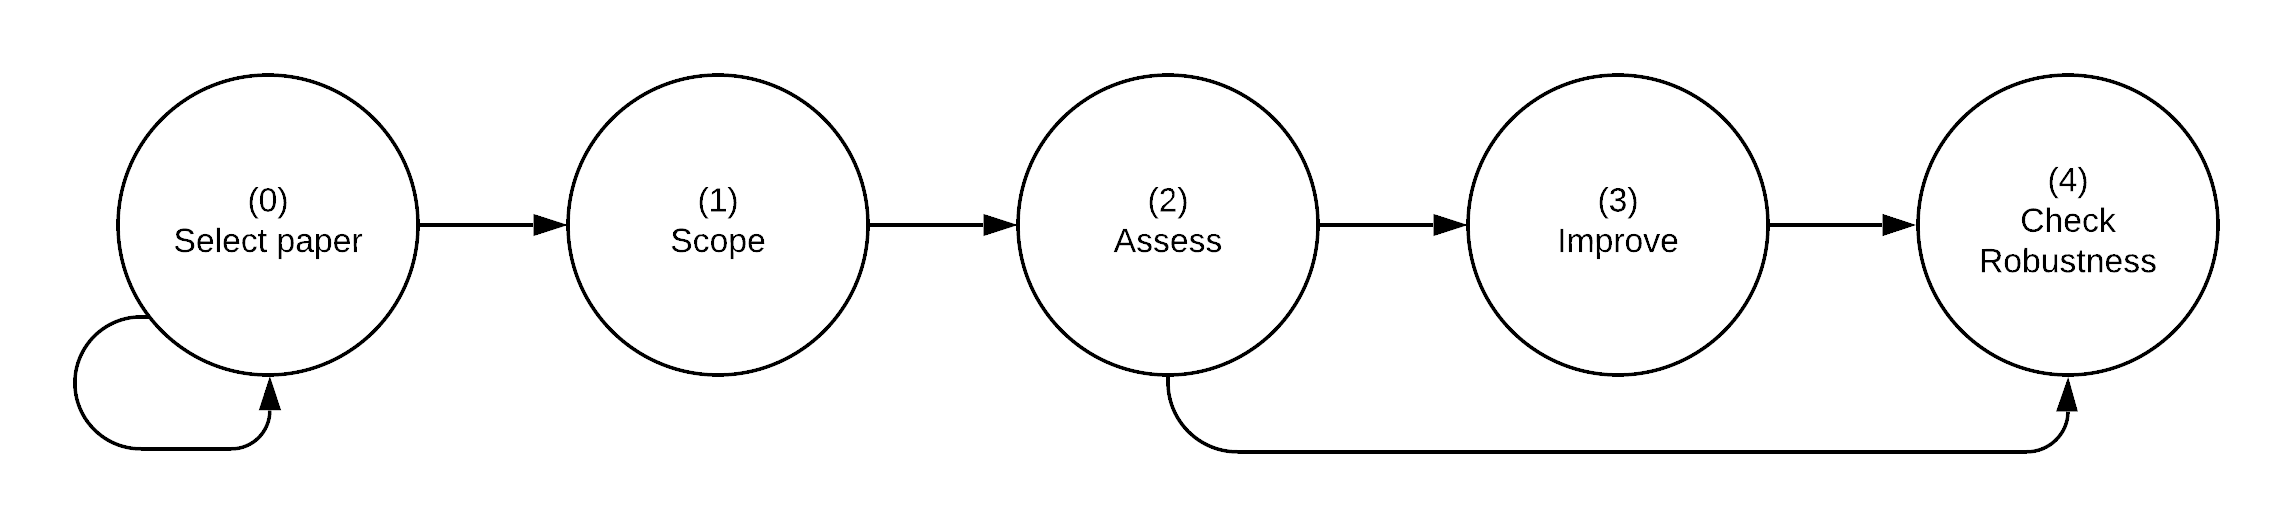
\includegraphics[width=1\linewidth]{images/stages}

\protect\hyperlink{select}{(0) Select}

\protect\hyperlink{scoping}{(1) Scoping}

\protect\hyperlink{assessment}{(2) Assessment}

\protect\hyperlink{improvements}{(3) Improvement}

\protect\hyperlink{robust}{(4) Robustness}

\protect\hyperlink{di-imp}{Display-item-level}

\protect\hyperlink{paper-level}{Paper-level}

☐ Select paper

\protect\hyperlink{read-summ}{☐ Read paper}

\protect\hyperlink{describe-inputs}{☐ Describe inputs}

\protect\hyperlink{rd}{☐ + Raw data}

\protect\hyperlink{paper-level}{☐ + Version control}

\protect\hyperlink{id-analy}{☐ Analytical choices}

\protect\hyperlink{declaree}{☐ Search materials}

\protect\hyperlink{declare-estimates}{☐ Identify claims}

\protect\hyperlink{diagram}{☐ Build reproduction diagrams}

\protect\hyperlink{ad}{☐ + Analysis data}

\protect\hyperlink{paper-level}{☐ + Documentation}

\protect\hyperlink{id-type}{☐ Type of choice}

\protect\hyperlink{check-acre}{☐ Check SSRP}

\protect\hyperlink{declare-estimates}{☐ Declare estimates}

\protect\hyperlink{score}{☐ Assign a reproducibility score}

\protect\hyperlink{ac}{☐ + Analysis code}

\protect\hyperlink{paper-level}{☐ + Dynamic document}

\protect\hyperlink{id-val}{☐ Choice value}

☐ Declare/Discard paper

\protect\hyperlink{cc}{☐ + Cleaning code}

\protect\hyperlink{paper-level}{☐ + File structure}

\protect\hyperlink{test-rob}{☐ Justify and test alternatives}

\protect\hyperlink{dac}{☐ Debug analysis code}

\protect\hyperlink{dcc}{☐ Debug cleaning code}

This work is licensed under the Creative Commons Attribution-NonCommercial 4.0 International License. To view a copy of this license, visit \url{http://creativecommons.org/licenses/by-nc/4.0/}.

\hypertarget{intro}{%
\chapter*{Introduction}\label{intro}}
\addcontentsline{toc}{chapter}{Introduction}

\emph{Computational reproducibility} is the degree to which it is possible to obtain consistent results using the same input data, computational methods, and conditions of analysis \citep{national2019reproducibility}. In 2019, the \href{https://www.aeaweb.org/journals/policies/data-code/}{American Economic Association} updated its Data and Code Availability Policy to require that the AEA Data Editor verify the reproducibility of all papers before they are accepted by an AEA journal. Similar policies have been adopted in political science, particularly at the \href{https://ajps.org/ajps-verification-policy/}{\emph{American Journal of Political Science}}. In addition to the requirements laid out in such policies, the data editors of several social science journals produced detailed \href{https://social-science-data-editors.github.io/guidance/}{recommendations and resources} to facilitate compliance. The goal of such policy changes is to improve the computational reproducibility of \emph{all} published research going forward, after several studies showed that rates of computational reproducibility in the social sciences range from somewhat low to alarmingly low \citep{galiani2018make, chang2015economics, kingi2018reproducibility}.

This Guide includes a common approach, terminology, and standards for conducting \emph{reproductions}, or attempts to assess and improve the computational reproducibility of published work. At the center of this process is the \emph{reproducer} (you!), a party rarely involved in the production of the original paper. Reproductions sometimes involve the \emph{original author} (whom we refer to as ``the author'') in cases where additional guidance and materials are needed to execute the process. Reproductions should be distinguished from \emph{replications}, where replicators re-examine a study's hypotheses using \emph{different data} or \emph{different methods} (or both) \citep{King95}. We find that reproducibility is necessary for replicability, though both allow science to be ``self-correcting.''

We recommend using this Guide in conjunction with the \href{https://www.socialsciencereproduction.org/}{\textbf{Social Science Reproduction Platform}} (SSRP), an open-source platform that crowdsources and catalogs attempts to assess and improve the computational reproducibility of published social science research. Though in its current version, the Guide is primarily intended for reproductions in economics, it may be used in other social science disciplines, and we welcome contributions that aim to ``translate'' any of its parts to other social science disciplines (learn how you can contribute \href{https://bitss.github.io/ACRE/contributions.html}{here}). Find definitions of fundamental concepts in reproducibility and the process of conducting reproductions in the \href{https://bitss.github.io/ACRE/definitions.html}{Glossary} chapter.

This Guide and the SSRP were developed as part of the Accelerating Computational Reproducibility in Economics \href{https://www.bitss.org/ecosystem/acre/}{(ACRE)} project, which aims to assess, enable, and improve the computational reproducibility of published economics research. The ACRE project is led by the Berkeley Initiative for Transparency in the Social Sciences \href{https://bitss.org}{(BITSS)}---an initiative of the Center for Effective Global Action \href{https://cega.berkeley.edu/}{(CEGA)}---and \href{https://www.vilhuber.com/lars/}{Dr.~Lars Vilhuber}, Data Editor for the journals of the American Economic Association (AEA). This project is supported by \href{https://www.arnoldventures.org/}{Arnold Ventures}.

\href{https://bitss.github.io/WEAI2020_slides/}{View slides used for the presentation ``How to Teach Reproducibility in Classwork''}

\hypertarget{beyond-binary-judgments}{%
\section*{Beyond binary judgments}\label{beyond-binary-judgments}}
\addcontentsline{toc}{section}{Beyond binary judgments}

Assessments of reproducibility can easily gravitate towards binary judgments that declare an entire paper as ``(ir-)reproducible''. We suggest a more nuanced approach by highlighting two realities that make binary judgments less relevant.

First, a paper may contain several scientific claims (or major hypotheses) that may vary in computational reproducibility. Each claim is tested using different methodologies, presenting results in one or more display items (outputs like tables and figures). Each display item will itself contain several specifications. Figure \ref{fig:diagram} illustrates this idea.

\begin{figure}
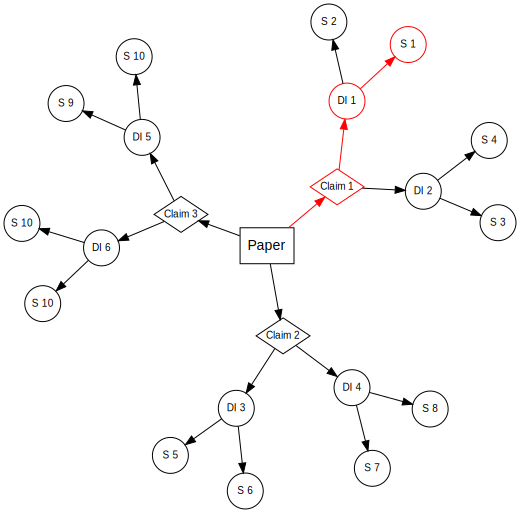
\includegraphics[width=1\linewidth]{images/paper-claims} \caption{One paper has multiple components to reproduce. <br> DI: Display Item, S: Specification }\label{fig:diagram}
\end{figure}

Second, for any given specification, there are several reproducibility levels, ranging from the absence of any materials to complete reproducibility starting from raw data. Moreover, even for a specific claim-specification combination, distinguishing the appropriate level can be far more constructive than simply labeling it as (ir-)reproducible.

Note that the highest level of reproducibility, which requires complete reproducibility starting from raw data, is very demanding and should not be expected of all published research --- especially before 2019. Instead, this level can serve as an aspiration for social science research, as we look to improve the reproducibility of research and facilitate the transmission of knowledge throughout the scientific community.

\hypertarget{reproduction-stages}{%
\section*{Reproduction stages}\label{reproduction-stages}}
\addcontentsline{toc}{section}{Reproduction stages}

Reproductions can be divided into five stages, corresponding to the first five chapters of this guide:

\begin{enumerate}
\def\labelenumi{\arabic{enumi}.}
\setcounter{enumi}{-1}
\tightlist
\item
  \protect\hyperlink{select}{\textbf{Paper selection}}, where you will select a \emph{candidate} paper and try to locate its \emph{reproduction package}. If a reproduction package is available, you will \emph{declare} the paper and start the reproduction, or select a new candidate paper (after leaving a record on the SSRP);\\
\item
  \protect\hyperlink{scoping}{\textbf{Scoping}}, where you will define the scope of the exercise by recording the claims, display items, and specifications you will focus on in the remainder of the reproduction;\\
\item
  \protect\hyperlink{assessment}{\textbf{Assessment}}, where you will review and describe in detail the available reproduction package and assess the current level of computational reproducibility of the selected display items;
\item
  \protect\hyperlink{improvements}{\textbf{Improvement}}, where you will modify the content and/or the organization of the reproduction package to improve its reproducibility;\\
\item
  \protect\hyperlink{robust}{\textbf{Robustness}}, where you will identify feasible robustness checks and/or assess the reasonableness of variations in analytical choices.
\end{enumerate}

This Guide does not include a possible fifth stage of \textbf{extension}, where you may extend the current paper by including new methodologies or data, which would bring the exercise closer to \emph{replication}.

\begin{figure}
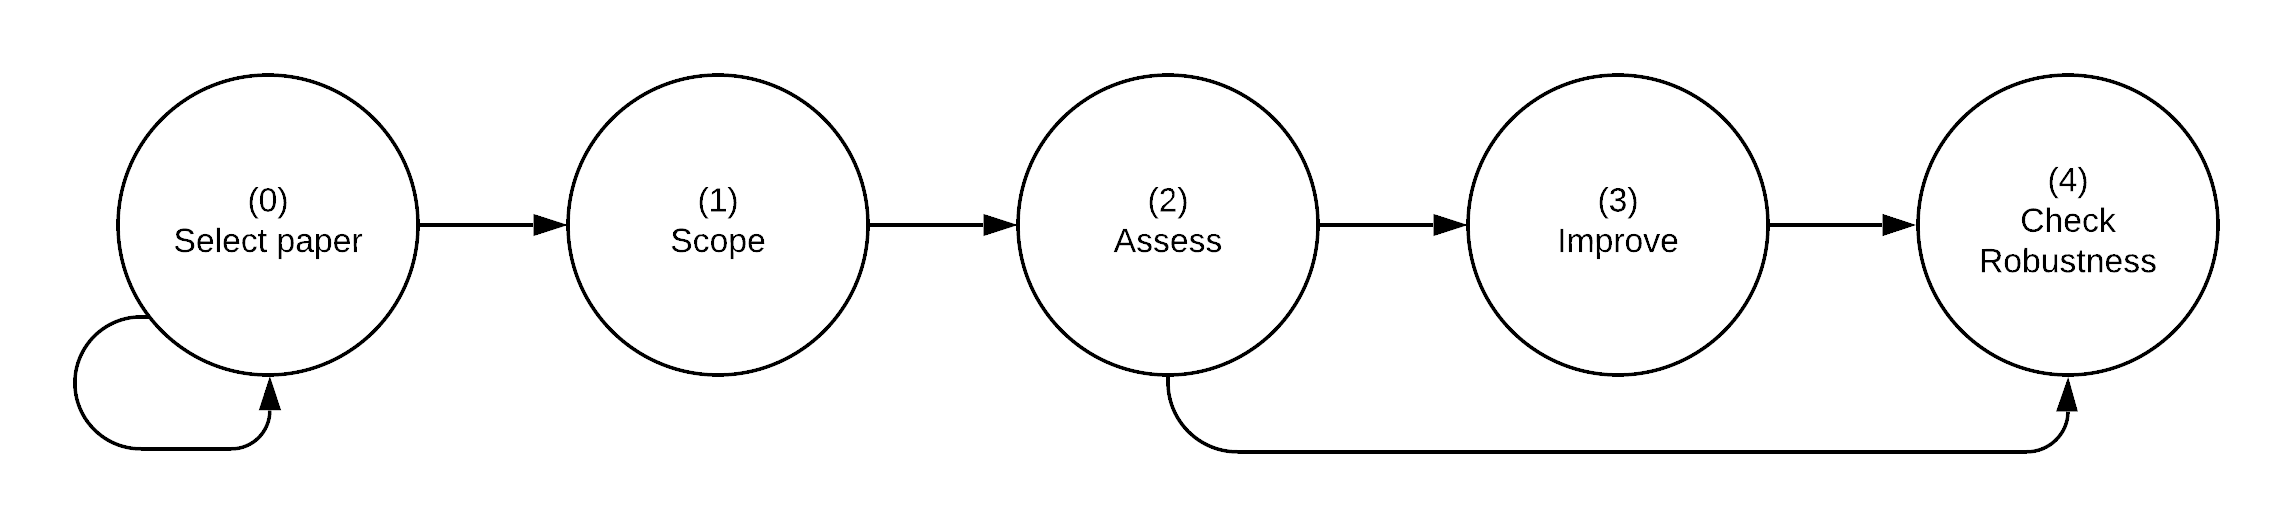
\includegraphics[width=1\linewidth]{images/stages} \caption{Four stages of a reproduction attempt}\label{fig:stages-intro}
\end{figure}

The order of the stages may not be chronologically linear. For example, you may realize that the scope of a reproduction is too ambitious and switch to a less intensive one. Later in the exercise, you can also begin testing different specifications for robustness while also assessing the paper's reproducibility level. The only stage that should go first, and cannot be edited once finished, is the Scoping stage.

Different stages in the reproduction process correspond to different units of analysis (see Figure \ref{fig:stages-unit} for an overview). E.g., the Scoping stage will focus on scientific \emph{claims} selected for reproduction. Once you specify your claims of interest, in the Assessment and Improvement stages you will focus on the display items associated with those claims. In the Robustness stage, claims are once again the unit of analysis.

\begin{figure}
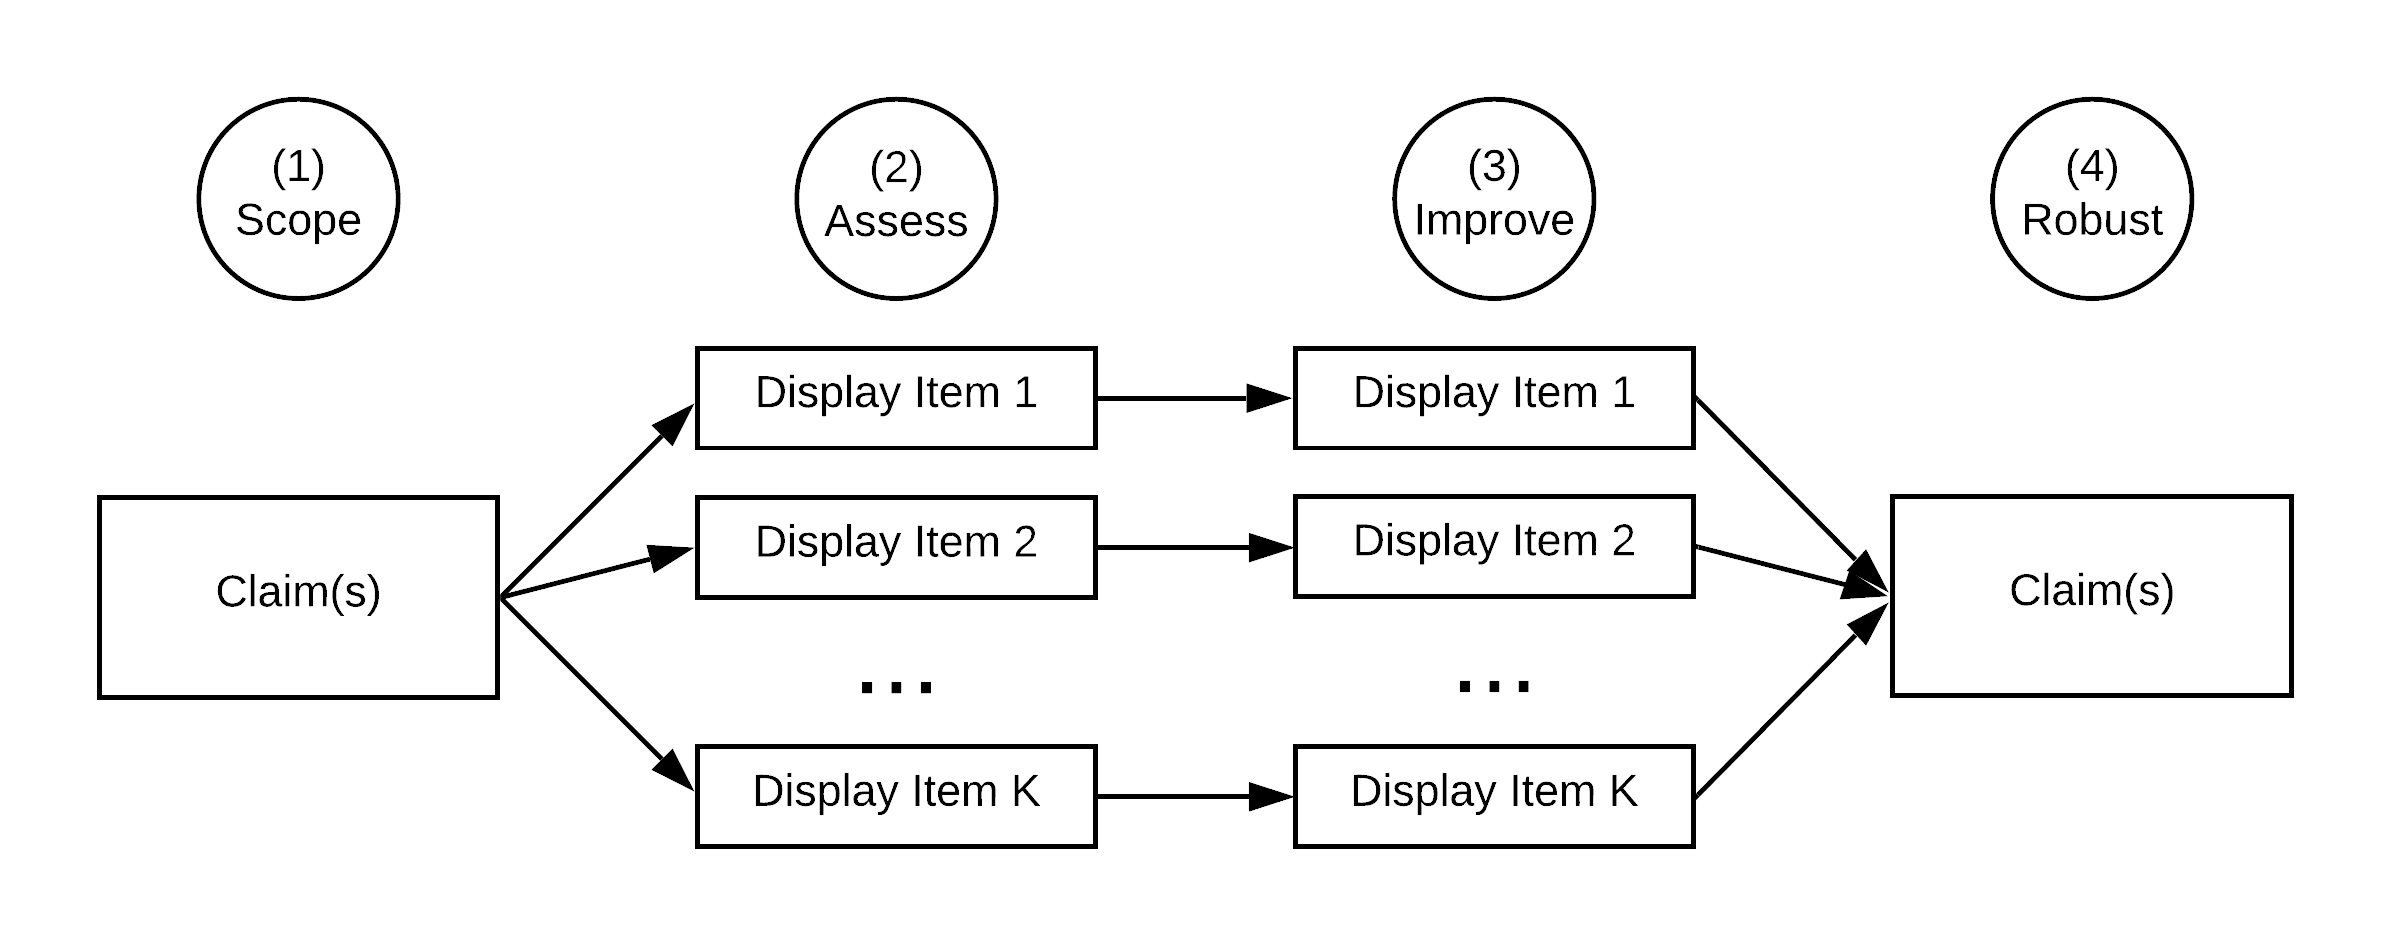
\includegraphics[width=1\linewidth]{images/unit-of-analysis} \caption{Relevant unit of analysis at each stage of a reproduction attempt}\label{fig:stages-unit}
\end{figure}

\hypertarget{reproduction-strategies}{%
\section*{Reproduction strategies}\label{reproduction-strategies}}
\addcontentsline{toc}{section}{Reproduction strategies}

In most cases, you will begin a reproduction with a thorough reading of your paper of interest. However, the sequence of the steps you take in the remainder of the reproduction may follow various \emph{reproduction strategies}. The most obvious strategy would be to follow the order of the steps as outlined above. You may also first choose one of the paper's many claims and then focus on assessing and improving the reproduction package accordingly. Using an alternative strategy, you might identify potential robustness checks or extensions while reading the paper and then focus only on the results associated with that robustness check. In another strategy, you may identify a paper that uses a particular dataset in which you are interested and then only reproduce or conduct robustness checks for the results associated with that dataset. The various uses of reproduction make the number of potential reproduction strategies potentially infinite, so it helps identify the goal of the reproduction from the start.

\hypertarget{select}{%
\chapter{Selecting a paper}\label{select}}

The goal of this stage is to help you define the scope of your exercise by declaring a paper and the specific output(s) on which you will focus. You might first consider multiple papers without analyzing them more closely (we refer to these as \textbf{candidate papers}) before moving forward with your \textbf{declared paper}.

The main difference between a candidate and a declared paper is the availability of a reproduction package. A \textbf{reproduction package} is the collection of materials that make it possible to reproduce a paper. This package may contain data, code, or documentation. If you are unable to independently locate the reproduction package for your paper, you can ask the paper's author for it (find guidance on this in \href{https://bitss.github.io/ACRE/guidance-for-a-constructive-exchange-between-reproducers-and-original-authors.html}{Chapter 7}) or simply choose another candidate paper. If you still want to explore the reproducibility of a paper with no reproduction package, these guidelines provide instructions for requesting materials from authors to create a public reproduction package, or if this proves unsuccessful, for building your reproduction package from scratch.

To avoid duplicating the efforts of others who may be interested in reproducing one of your candidate papers, \textbf{we ask that you record your candidate papers in the SSRP database} (currently under development).

Note that in this stage, \emph{you are not expected to review the reproduction materials in detail}, as you will dedicate most of your time to this in later stages of the exercise.

\hypertarget{declare}{%
\section{From candidate to declared paper}\label{declare}}

At this point of the exercise, you are \emph{only validating the availability} of (at least) one reproduction package and not assessing the quality of its content. Follow the steps below to verify that a reproduction package is available, and stop whenever you find it (this may mean that you have found your declared paper).

\begin{enumerate}
\def\labelenumi{\arabic{enumi}.}
\tightlist
\item
  Check whether previous reproduction attempts have been recorded in the SSRP Database for the paper (more on the SSRP Database in the next section).
\item
  Check the journal or publisher's website, looking for materials named ``Data and Materials,'' ``Supplemental Materials,'' ``Reproduction/Replication Package/Materials,'' etc.\\
\item
  Look for links in the paper (review the footnotes and appendices).\\
\item
  Review the personal websites of the paper's author(s).
\item
  Contact the author(s) to request the reproduction package using \href{https://bitss.github.io/ACRE/guidance-for-a-constructive-exchange-between-reproducers-and-original-authors.html\#contacting-the-original-authors-when-there-is-no-reproduction-package}{this} email template. In this and future interactions with authors, we encourage you to follow our guidance outlined in \href{https://bitss.github.io/ACRE/guidance-for-a-constructive-exchange-between-reproducers-and-original-authors.html\#contacting-the-original-authors-when-there-is-no-reproduction-package}{Chapter 7}.
\item
  Deposit the reproduction package in a trusted repository (e.g., \href{https://dataverse.org/}{Dataverse}, \href{https://www.openicpsr.org/openicpsr/}{Open ICPSR}, \href{https://zenodo.org/}{Zenodo}, or the \href{https://osf.io/}{Open Science Framework}) under the name \texttt{Original\ reproduction\ package\ for\ -\ Title\ of\ the\ paper}. You will be asked to provide the URL of the repository in Survey 1.
\end{enumerate}

In case you need to contact the authors, make sure to \emph{allocate sufficient time for this step} (we suggest at least three weeks before the date you plan to start the reproduction). Instructors should also plan to accordingly (e.g., if the ACRE exercise is expected to take place in the middle of the semester, students should review candidate papers and (if applicable) contact the authors in the first few weeks of the semester).

Review the decision tree (Figure \ref{fig:candidate-paper-dec-tree}) below for a more detailed overview of this process. Remember, \emph{if at any step of the process you decide to abandon the paper, make sure to record the candidate paper in the ACRE database} before moving on to another candidate paper. Once you have obtained the reproduction package, the \emph{candidate paper} becomes your \emph{declared paper} and you can move forward with the exercise! Do not invest time in doing a detailed read of any paper until you are sure that it is your declared paper.

\hypertarget{check-acre}{%
\subsection{Candidate paper entries in the SSRP Database}\label{check-acre}}

If the SSRP database contains previous reproduction attempts of the paper, you will see a report card with the following information:

\begin{quote}
\textbf{Box 1:} Summary Report Card for ACRE Paper Entry\\
\textbf{Title:} Sample Title\\
\textbf{Authors:} Jane Doe \& John Doe\\
\textbf{Original Reproduction Package Available:} Yes (link)/No.\\
{[}If ``No''{]} \textbf{Contacted Authors?:} Yes/No\\
{[}If ``Yes(contacted)''{]} \textbf{Type of Response:} Categories (6).\\
\textbf{Additional Reproduction Packages:} Number (eg., 2)\\
\textbf{Authors Available for Further Questions for ACRE Reproductions:} Yes/No/Unknown
\end{quote}

If after taking steps 1-5 above (or for some other reason) you are unable to locate the reproduction package, record your candidate paper (and if applicable, the outcome of your correspondence with the original authors) in the SSRP database following the example above.

\begin{figure}
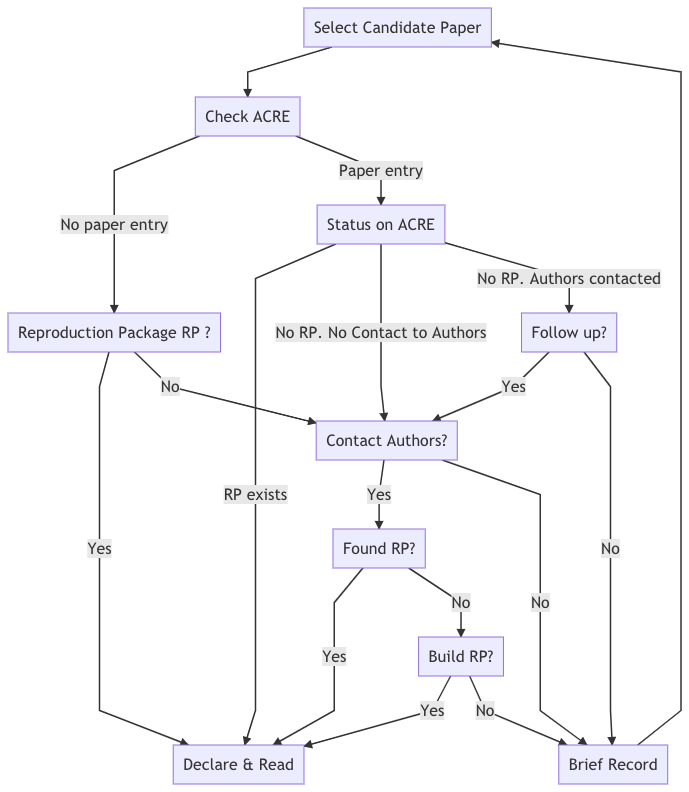
\includegraphics[width=0.8\linewidth]{images/candidate-to-declared-paper} \caption{Decision tree to move from candidate to declared paper}\label{fig:candidate-paper-dec-tree}
\end{figure}

\hypertarget{identify-timeline}{%
\section{Identifying the relevant timeline}\label{identify-timeline}}

Before you begin working on the four main stages of the reproduction exercise (Scoping, Assessment, Improvement, and Robustness), it is important to manage your own expectations and those of your instructor or advisor. Be mindful of your time limitations when defining the scope of your reproduction activity. These will depend on the type of exercise chosen by your instructor or advisor and may vary from a weeklong homework assignment, to a longer class project that may take a month to complete or a semester-long project (an undergraduate thesis, for example).

Table 1 shows an example distribution of time across three different reproduction formats. The Scoping and Assessment stages are expected to last roughly the same amount of time across all formats (lasting longer for the semester-long activities, and acknowledging that less experienced researchers, such as undergraduate students, may need more time). Differences emerge in the distribution of time for the last two main stages: Improvements and Robustness. For shorter exercises, we recommend avoiding any possible improvements to the raw data (or cleaning code). This will limit how many robustness checks are possible (for example, by limiting your ability to reconstruct variables according to slightly different definitions), but it should leave plenty of time for testing different specifications at the analysis level.

2 weeks (\textasciitilde10 days)

1 month (\textasciitilde20 days)

1 semester (\textasciitilde100 days)

analysis data

raw data

analysis data

raw data

analysis data

raw data

Scoping

10\% (1 day)

5\% (1 day)

5\% (5 days)

Assessment

35\%

25\%

15\%

Improvement

25\%

0\%

40\%

20\%

30\%

Robustness

25\%

5\%

25\%

25\%

\hypertarget{scoping}{%
\chapter{Scoping}\label{scoping}}

At this stage, you will define the \emph{scope of the reproduction} by identifying the \emph{scientific claims} and related \emph{display items} that you will analyze in the remainder of the reproduction. For this exercise, we follow the a comparable definition of a claim as used in the SCORE project, a related initiative aimed at predicting replicability and reproducibility of research:

\begin{quote}
``A research claim is a single major finding from a published study, as well as details of the methods and results that support this finding. A research claim {[}may not be{]} equivalent to an entire article. Sometimes the claim as described in the abstract does not exactly match the claim that is tested. In this case, you should consider the research claim to be that which is described in the {[}results of the paper{]}''.

-- \href{https://replicats.research.unimelb.edu.au/\#tab301}{RepliCATS Project}
\end{quote}

In the SSRP framework, different claims in a paper may be tested using different methodologies, and their results may be presented in one or more display items, such as tables and figures (\href{https://bitss.github.io/ACRE/intro.html\#fig:diagram}{figure 0.1} illustrates this idea). There are several types of claims, including:

\begin{itemize}
\item
  \textbf{Causal claim:} An assertion that invokes causal relationships between variables. A paper may estimate the effect of \emph{X} on \emph{Y} for population \emph{P}, using method \emph{F}. E.g., ``This paper investigates the impact of bicycle provision on secondary school enrollment among young women in Bihar/India, using a Difference in Difference approach.''
\item
  \textbf{Descriptive/predictive claim:} An assertion that estimates the value of \emph{Y} (estimated or predicted) for population \emph{P} under dimensions \emph{X} using method \emph{M}. E.g., ``Drawing on a unique Swiss data set (population \emph{P}) and exploiting systematic anomalies in countries' portfolio investment positions (method \emph{M}), I find that around 8\% of the global financial wealth of households is held in tax havens (value of \emph{Y}).''
\end{itemize}

A \emph{display item} is a figure or table that presents the results described in the paper. Each display item contains several \emph{specifications}.

When recording the Scoping section on the SSRP platform, count all of the claims in the paper and provide a one sentence summary for the subset of claims that you will attempt to reproduce. Structure your summary as follows: ``The paper tested the effect of X on Y for population P, using method F. The main results show an effect of magnitude E (specify units and standard errors)'' or ``The paper estimated the value of Y (estimated or predicted) for population P under dimensions X using method M. The main results presented an estimate of of magnitude E (specify units and standard errors)''. Make sure to use the same units of measurement for all scientific claims that you will analyze as part of the reproduction.

\textbf{Note:} Once you progress past the Scoping stage on the SSRP, \emph{you will no longer be able to edit your responses in the Scoping stage}, though you will be able to see them. This is because the content of later stages of the reproduction is dependent on the information you record at this stage of the reproduction.

\hypertarget{read-sum}{%
\section{Read and summarize the paper}\label{read-sum}}

Depending on your reproduction's timeline, we recommend that you write a short (\textless1000 words) summary of the paper. Writing up such a summary will help you develop and demonstrate a wholesome understanding of the paper and its various components. In your summary, try to address the following:

\begin{itemize}
\tightlist
\item
  How many scientific claims can you identify in the paper?
\item
  Would you classify the claims as causal, descriptive (e.g., estimating a population's descriptive statistic), or something else?\\
\item
  What is the population that is the focus of the paper as a whole?\\
\item
  What is the population for which the estimates apply?\\
\item
  What are the primary data sources used in the paper?\\
\item
  What is the primary statistical or econometric method used to examine each claim?\\
\item
  What is the author's preferred specification (or yours, if the authors' is unclear)?\\
\item
  What are some possible robustness checks for the preferred specification?\\
\item
  How many display items are there in the paper (tables, figures, and inline results)?
\end{itemize}

Draft the summary in a plain text editor and paste the text in the form.

\hypertarget{record-a-revised-reproduction-package}{%
\section{Record a revised reproduction package}\label{record-a-revised-reproduction-package}}

At the previous stage, you recorded the original reproduction package made available by the paper's authors. Given that one of the main goals of the ACRe approach is to improve reproducibility, we recommend that you build an alternative reproduction package that will improve the reproducibility of specific display items or the paper as a whole.
You can start by downloading the reproduction package (or \emph{forking}, if on GitHub) and uploading a copy titled ``Revised reproduction package for {[}Paper Citation, e.g.~Smith et al.~(2019){]}'' to a trusted repository. Examples of trusted repositories include \href{https://dataverse.org/}{Dataverse}, \href{https://www.openicpsr.org/openicpsr/}{openICPSR}, \href{https://figshare.com}{Figshare}, \href{https://datadryad.org/stash}{Dryad}, \href{https://about.zenodo.org/}{Zenodo}, \href{osf.io/}{Open Science Framework} and others. We encourage you to also use version control software (e.g., Git) during your reproduction.

Trusted repositories have a file size limit (typically around 2gb). If you think that your reproduction package will exceed this limit please do the following:

\begin{itemize}
\tightlist
\item
  Separate your reproduction package in two: (1) data and (2) code and documentation.\\
\item
  Post the second one in a trusted repository.\\
\item
  For the data reproduction package identify all the files that are different from the original reproduction package and upload only those. For example, suppose the original repro package has \texttt{data/raw\_data1.csv}, and \texttt{data/clean\_data/data\_set1.dta}. If you modify only the file \texttt{data\_set1.dta}, then upload a revised reproduction package that has the same folder structure but only the files that differ: \texttt{data/clean\_data/data\_set1.dta}. If you want to make it even more clear you could add a readme file describing the modified files.
\end{itemize}

As you work through the next stages, you can modify the reproduction package and record your improvements on the SSRP. Keeping a record of such changes will help you document your assessments or communicate with the original authors, and it will also allow future reproducers to build on top of your work.

\hypertarget{declare-estimates}{%
\section{Record scope of the exercise}\label{declare-estimates}}

By now, you probably have a reasonably good understanding of the paper. You do not, however, need to spend any time reviewing the reproduction package in detail.

At this point, you should specify the parts of the paper that will be the main focus of your reproduction. Focus on specific estimates, represented by a unique combination of claim-display item-specification as represented in figure \ref{fig:diagram}. Given the complexity of the SSRP approach, unless you are very familiar with the paper, we recommend starting with just one claim before moving onto second or third as part of a later reproduction.

\hypertarget{declare-a-specific-estimates-to-reproduce}{%
\subsubsection*{Declare a specific estimate(s) to reproduce}\label{declare-a-specific-estimates-to-reproduce}}
\addcontentsline{toc}{subsubsection}{Declare a specific estimate(s) to reproduce}

Identify a scientific claim and its corresponding preferred specification and record its magnitude, standard error, and location in the paper (page, table \#, and table row and column). If the authors did not explicitly choose a precise preferred estimate, you can choose one yourself. In addition to the preferred estimate, you can reproduce up to five estimates that correspond to the preferred estimate's alternative specifications.

\hypertarget{declare-possible-robustness-checks-for-main-estimates-optional}{%
\subsubsection*{Declare possible robustness checks for main estimates (optional)}\label{declare-possible-robustness-checks-for-main-estimates-optional}}
\addcontentsline{toc}{subsubsection}{Declare possible robustness checks for main estimates (optional)}

After reading the paper, you might wonder why the authors did not conduct a specific robustness test. If you think that such analysis could have been done \emph{within the same methodology} and \emph{using the same data} (e.g., by including or excluding a subset of the data like ``high-school dropouts'' or ``women''), please specify a robustness test that you would like to conduct before starting the Assessment stage. Robustness checks in this stage are \emph{optional} and can take the form of a short sentence describing at a high level what you (the reproducer) would like to explore in a later stage. In the robustness stage (after assessment and improvement) you will be able to describe in greater detail how you have modified the reproduction code.

\hypertarget{assessment}{%
\chapter{Assessment}\label{assessment}}

In the \emph{Assessment} stage, you will describe the available reproduction materials and assign a reproducibility score to the display items associated with your selected claims. You will also review reproducibility practices for the overall paper. This stage records rich information about each reproduction to allow future reproducers to pick up easily where others have left off.

In the previous two stages, you declared a paper and identified claims and their associated estimates (found in display items) that you intend to analyze in the remainder of your reproduction. In this stage, you will get to decide whether you are interested in assessing the reproducibility of entire display items (e.g., ``Table 1'') or only specific estimates found in display items (e.g., ``rows 3 and 4 of Table 1''). You can also include additional display items of interest.

The Assessment stage aims to analyze the reproduction package's \emph{current} reproducibility---before you suggest any improvements. By the end of this section, you will have created a very detailed description of the reproduction package's current reproducibility that you can use to implement improvements, potentially with the paper's original authors' help.

On the SSRP, you will first provide a detailed description of available inputs in the reproduction package. You will then connect the display items you've chosen to reproduce with their corresponding inputs. With these elements in place, you can assign a score of each display item's reproducibility and record various paper-level dimensions of reproducibility.

\emph{Tip:} We recommend that you first focus on just one display item (e.g., ``Table 1''). After completing the assessment for this display item, you will have a much easier time assessing others.

\hypertarget{describe-inputs}{%
\section{Describe the inputs}\label{describe-inputs}}

This section explains how to record the \emph{input} materials found (or referenced) in the reproduction package. At this point, it may be challenging to precisely identify the materials that correspond to your selected claims and display items, so we recommend listing \emph{all} files in the reproduction packages (\emph{tip}: using the command line, go to the directory of the reproduction package, and type \texttt{file\ */*} on a Mac or \texttt{dir\ /s\ /b\ /o:gn} on Windows to obtain a printout of all files within a folder). However, if the reproduction package is too extensive to record in its entirety, you can focus only on the materials required to reproduce a specific display item.

The following concepts may be helpful as you work in the Assessment stage (also see the ACRe glossary \href{https://bitss.github.io/ACRE/definitions.html}{here}):

\begin{itemize}
\tightlist
\item
  \textbf{Raw data} -- Unmodified data files obtained by the authors from the sources cited in the paper. Data from which personally identifiable information (PII) has been removed are \emph{still considered raw}. All other modifications to raw data make it \emph{processed}.\\
\item
  \textbf{Analysis/Analytic data} -- Data used as the final input in a workflow to produce a statistic displayed in the paper (including appendices).\\
\item
  \textbf{Cleaning code:} A script associated primarily with data cleaning. Most of its content is dedicated to actions like deleting variables or observations, merging data sets, removing outliers, or reshaping the data structure (from long to wide, or vice versa).\\
\item
  \textbf{Analysis code:} A script associated primarily with analysis. Most of its content is dedicated to generate some type of estimate to be presented in the paper (including the appendix). Examples of computations that lead to such estimates are: running regressions, running hypothesis tests, computing standard errors, and imputing missing values.
\end{itemize}

In section ``Describe input'' on the SSRP, you can record data sources and connect them with their raw data files (if available). You can then locate and provide a brief description of the analytic data files and then record script files in Table.

\emph{Tip:} For large volume of data sources, we recommend downloading the empty table as a CSV file, recording the information in the downloaded file, and uploading the final version of the document to populate the table.

\hypertarget{desc-sourc}{%
\subsection{Describe the data sources and raw data}\label{desc-sourc}}

In the paper you chose, find references to all \emph{data sources} used in the analysis. A data source is usually described in narrative form. For example, if in the body of the paper, or the appendix, you see text like ``(\ldots) for earnings in 2018 we use the Current Population Survey'', the data source is ``2018 Current Population Survey''. If the first reference to this data source is found on page 1 of the appendix, you should record its location as ``A1''. Do this for all data sources mentioned in the paper. Each row represents a unique data source.

Data sources also vary by unit of analysis, with some sources matching the same unit of analysis used in the paper (as in previous examples). In contrast, others may be less clear, e.g., ``our information on regional minimum wages comes from the Bureau of Labor Statistics.'' You should record such data source as ``regional minimum wages from the Bureau of Labor Statistics.''

Next, look at the reproduction package and map the \emph{data sources} mentioned in the paper to the \emph{Data Files} in the reproduction package. In the \emph{Location} column, record their folder locations relative to the main reproduction folder\footnote{a relative location takes the form of \texttt{folder\_in\_rep\_materials/sub\_folder/file.txt}, in contrast to an absolute location that takes the form of \texttt{/username/documents/projects/repros/folder\_in\_rep\_materials/sub\_folder/file.txt}}. In addition to looking at the existing data files, we recommend that you also review the first lines of all code files (especially cleaning code), looking for lines that call the datasets. Inspecting these scripts may help you understand how different data sources are used, and possibly identify any missing files from the reproduction package. Whenever a data source contains multiple files, enter them in the same cell, separated by semicolon (\texttt{;}).

If you cannot find the files or file name corresponding to a specific data source, type ``Missing'' in the \emph{Notes} column. Check the \emph{Provided} column if the data source was included in the original reproduction package. Check the \emph{Cited} column if the data source was explicitly cited in the paper. Record your work using the following structure:

\begin{table}

\caption{\label{tab:raw-data-information}Raw data information}
\centering
\begin{tabu} to \linewidth {>{\raggedright}X>{\raggedright}X>{\raggedright}X>{\raggedright}X>{\raggedright}X>{\raggedright}X>{\raggedright}X}
\hline
data\_source & page & data\_files & directory & known\_missing & provided & cited\\
\hline
"Current Population Survey 2018" & A1 & cepr\_march\_2018.dta & data/ &  & TRUE & FALSE\\
\hline
"Provincial Administration Reports" & A4 & coast\_simplepoint2.csv; rivers\_simplepoint2.csv; RAIL\_dummies.dta; railways\_Dissolve\_Simplify\_point2.csv & Data/maps/ &  & TRUE & FALSE\\
\hline
"2017 SAT scores" & 4 & Not available & data/to\_clean/ &  & FALSE & TRUE\\
\hline
... & ... & ... & ... & ... & ... & ...\\
\hline
\end{tabu}
\end{table}

\hypertarget{desc-analy}{%
\subsection{Describe the analytic data}\label{desc-analy}}

First, identify all analytic data files in the reproduction package and record their names in the \emph{Analytic Data} column in Table 1.2. You will recognize analytic data files based on the documentation, their location folder, or if a code file produces them.

Second, record each analytic data file's location relative to the main folder of the reproduction package in the \emph{Location} column.

Finally, provide a one-line description of each file in the \emph{Description} column (e.g., all\_waves.csv can be ``data for region-level analysis''). This will become easier as you progress through the reproduction, and you can always return to this table later on and add or modify your descriptions.

The resulting table may look like this:

\begin{table}

\caption{\label{tab:analysis-data-information}Analysis data information}
\centering
\begin{tabu} to \linewidth {>{\raggedright}X>{\raggedright}X>{\raggedright}X}
\hline
analysis\_data & location & description\\
\hline
final\_data.csv & analysis/fig1/ & data for figure1\\
\hline
all\_waves.csv & final\_data/v1\_april/ & data for region-level analysis\\
\hline
... & ... & ...\\
\hline
\end{tabu}
\end{table}

\emph{Note on data citations}: Assessment of whether or not a data source has been cited should take into account the general guidelines for what is considered a complete data citation. In-text citations, mention of the source location (e.g.~url to source location), description of the source or the data alone are examples of incomplete data citations. Please refer to the \href{https://social-science-data-editors.github.io/guidance/addtl-data-citation-guidance.html\#generic-guidance}{Guidance on Data Citations by Social Science Data Editors} for a comprehensive overview and more reference material on data citation standards for the social sciences.

\hypertarget{desc-scripts}{%
\subsection{Describe the code scripts}\label{desc-scripts}}

First, identify all code files in the reproduction package and record their names in the \emph{File Name} column and record their locations relative to the main folder in the \emph{Location} column.

Then, review the beginning and end of each code file to identify the inputs required to successfully run the file and the outputs it produces. Inputs are data sets or other code scripts that are typically found at the beginning of the script (e.g., `load', `read', `source', `run', `do'). Outputs are other data sets, or plain text files typically found at the end of a script (e.g., 'save, write, export). Record those in the \emph{Inputs} and \emph{Outputs} columns.

Finally, provide a brief description of the code's function in the \emph{Description} column and classify its function as analysis or cleaning and/or construction in the \emph{Primary Type} column.

For each code file, record all outputs together and separate each item with (\texttt{;}). Record all of this information in the SSRP using the following structure:

\begin{table}

\caption{\label{tab:code-files-information}Code files information}
\centering
\begin{tabu} to \linewidth {>{\raggedright}X>{\raggedright}X>{\raggedright}X>{\raggedright}X>{\raggedright}X>{\raggedright}X}
\hline
file\_name & location & inputs & outputs & description & primary\_type\\
\hline
output\_table1.do & code/analysis/ & analysis\_data01.csv & output1\_part1.txt & produces first part of table 1 (unformatted) & analysis\\
\hline
data\_cleaning02.R & code/cleaning & admin\_01raw.csv & analysis\_data02.csv & removes outliers and missing vals from raw admin data & cleaning\\
\hline
... & ... & ... & ... & ... & ...\\
\hline
\end{tabu}
\end{table}

\hypertarget{common-issues-that-might-occur-when-creating-a-reproduction-tree}{%
\subsubsection{Common issues that might occur when creating a reproduction tree:}\label{common-issues-that-might-occur-when-creating-a-reproduction-tree}}

\begin{itemize}
\item
  If you notice that some files iterate between each other (e.g., \texttt{file1.do} calls \texttt{data1.csv} to generate \texttt{data2.csv}, and \texttt{file2.R} calls \texttt{data2.csv} to generate \texttt{data1.csv}), look within the files to identify the one that contains some stopping criteria (e.g., stop when SSR is minimized). Then designate only one output as the final and record that in reproduction diagram in the next section.
\item
  Sometimes the reproduction package will not produce display items as its final outputs. In this situation, the final code script will generate some type of output (e.g., \texttt{results1.log}, \texttt{results2.csv}) that will require manual copying and pasting to reproduce the desired display item (e.g.~\texttt{Table\ 1}). In this case, we recommend adding one auxiliary line to the table linking the final output to the desired display item (e.g., File Name: aux1, Inputs: \texttt{results1.log;\ results2.csv}, Outputs: \texttt{Table\ 1}).
\item
  Some reproduction packages might have a large number of files that follow a recurrent structure (e.g., \texttt{data\_location1\_year1,\ data\_location2\_year1,\ data\_location1\_year2,\ ...}). To make a more tractable tree we recommend that you record the names of these files only once and use a consistent place holder (e.g., \texttt{data\_locationX\_yearY}).
\item
  If the reproduction tree shows several files under one input, make sure that each file is separated by a semi-colon (\texttt{;}), that way the tree will separate each file into a separate input.
\end{itemize}

\hypertarget{diagram}{%
\section{Connect display items to all its inputs usign the ReproducibiliTREE}\label{diagram}}

Using the information above, the SSRP will build a diagram that can help you visually trace your display items to the code and data files that produce them. If the reproduction package does not organize the code around display items, you can identify all of the outputs that contain the results used in a specific display item.

\hypertarget{complete-tree}{%
\subsection{Complete workflow information}\label{complete-tree}}

If you were able to identify all of the relevant components in the previous section, the ReproducibiliTREE will produce a tree diagram that looks similar to the one below.

\begin{verbatim}
  table1.tex
      └──[code] analysis.R
          └──analysis_data.dta
              └──[code] final_merge.do
                  └──cleaned_1_2.dta
                  |   └──[code] clean_merged_1_2.do
                  |       └──merged_1_2.dta
                  |           └──[code] merge_1_2.do
                  |               └──cleaned_1.dta
                  |               |   └──[code] clean_raw_1.py
                  |               |       └──raw_1.dta
                  |               └──cleaned_2.dta
                  |                   └──[code] clean_raw_2.py
                  |                       └──raw_2.dta
                  └──cleaned_3_4.dta
                      └──[code] clean_merged_3_4.do
                          └──merged_3_4.dta
                              └──[code] merge_3_4.do
                                  └──cleaned_3.dta
                                  |   └──[code] clean_raw_3.py
                                  |       └──raw_3.dta
                                  └──cleaned_4.dta
                                      └──[code] clean_raw_4.py
                                          └──raw_4.dta
\end{verbatim}

This diagram, built with the information you provided, contributes to understanding the necessary components required to reproduce a specific display item. It also summarizes key information to allow for more constructive exchanges with original authors or other reproducers. For example, when contacting the authors for guidance, you can use the diagram to ask for specific files. Formulating your request this way makes it easier for authors to respond and demonstrates that you understand the reproduction package. You can also add this diagram to the readme of your revised reproduction package.

\hypertarget{incomplete-workflow-information}{%
\subsection{Incomplete workflow information}\label{incomplete-workflow-information}}

In some cases, some of the workflow components may not be easily identifiable in the reproduction package (or might be missing). Here the ReproducibiliTREE will return a fagmented reproduction tree diagram. See below how you can work around such cases, but even if the reproduction tree is fragmented, you can still go on to the next step of the reproduction.

For example, here's a simple complete reproduction tree:

\begin{verbatim}
  table1.tex
    └── analysis.R
        └── analysis_data.dta
            └── final_merge.do
                └── cleaned_1_2.dta
                   └── clean_merged_1_2.do
                       └── merged_1_2.dta
\end{verbatim}

For this case, if the the file \texttt{final\_merge.do} is missing, the ReproducibiliTREE will produce the following reproduction tree:

\begin{verbatim}
  table1.tex
    └── analysis.R
        └── analysis_data.dta

  cleaned_1_2.dta
    └── clean_merged_1_2.do
        └── merged_1_2.dta
\end{verbatim}

You can still manually combine this partial information with your knowledge from the paper and own (subjective) judgement to produce a ``candidate'' reproduction tree. This may look like the following:

\begin{verbatim}
  table1.tex
    └── analysis.R
        └── cleaned_1_2.dta
            └── MISSSING_CODE_FILE_1
                └── cleaned_1_2.dta
                   └── clean_merged_1_2.do
                       └── merged_1_2.dta
\end{verbatim}

If you notice that the reproduction tree is fragmented where it shouldn't be, you may need to amend Table 1.3 above with placeholders. In the example above, that can look like this:

\begin{table}

\caption{\label{tab:adding-rows}Adding rows to code spreadsheet}
\centering
\begin{tabu} to \linewidth {>{\raggedright}X>{\raggedright}X>{\raggedright}X>{\raggedright}X>{\raggedright}X>{\raggedright}X}
\hline
file\_name & location & inputs & outputs & description & primary\_type\\
\hline
... & ... & ... & ... & ... & ...\\
\hline
MISSSING\_CODE\_FILE\_1 & unknown & cleaned\_1\_2.dta & cleaned\_1\_2.dta & missing code & unknown\\
\hline
\end{tabu}
\end{table}

As in the cases with complete workflows, these diagrams (fragmented or reconstructed trees) provide important information for assessing and improving the reproducibility of specific display items. For more examples of diagrams connecting final outputs to initial raw data, \protect\hyperlink{examples-of-reproduction-trees}{see here}.

\hypertarget{score}{%
\section{Assign a reproducibility score.}\label{score}}

Once you have identified all possible inputs and have a clear understanding of the connection between the display items and their inputs, you can assign reproducibility scores to individual display items.

The following concepts may be helpful in this section:

\begin{itemize}
\item
  \textbf{Computationally Reproducible from Analytic data (CRA)} --- The output can be reproduced with minimal effort starting from the \emph{analytic} datasets.
\item
  \textbf{Computationally Reproducible from Raw data (CRR)} --- The output can be reproduced with minimal effort from the \emph{raw} datasets.
\item
  \textbf{Standard of \emph{minimal effort}} --- One hour or less is required to run the code, not including computing time.
\end{itemize}

\hypertarget{levels-of-computational-reproducibility-for-a-specific-output}{%
\subsection{Levels of Computational Reproducibility for a Specific Output}\label{levels-of-computational-reproducibility-for-a-specific-output}}

Each level of computational reproducibility is defined by the availability of data and materials, and whether the available materials faithfully reproduce the display item of interest. The description of each level also includes possible improvements that can help advance the display item's reproducibility. You will learn in more detail about the possible improvements at the \href{https://bitss.github.io/ACRE/improvements.html}{\emph{Improvement} stage}.

Note that the assessment is made \emph{at the level of individual display items}---a paper can be highly reproducible for its main results, but its other display items may not be as reproducible. The assessment includes a 10-point scale, where 1 represents that, under the current circumstances, reproducers cannot access any reproduction package. At level 10, the reproducer can access all of the necessary materials to faithfully reproduce the target display item from the raw data.

\begin{itemize}
\tightlist
\item
  \textbf{Level 1 (L1):} No data or code are available. Possible improvements include adding: raw data, analysis data, cleaning code, and analysis code.
\end{itemize}

You may have detected papers without any reproduction materials at the \emph{Paper Selection} stage, where you should have recorded them as unsuccessful candidate papers.

\begin{itemize}
\item
  \textbf{Level 2 (L2):} Code scripts are available (partial or complete), but no data are available. Possible improvements include adding: raw data and analysis data.
\item
  \textbf{Level 3 (L3):} Analytic data and code are partially available, but raw data and cleaning code are missing. Possible improvements include: completing analysis data and/or code, adding raw data, and adding analysis code.
\item
  \textbf{Level 4 (L4):} All analytic data sets and analysis code are available, but the code fails to run or produces results inconsistent with the paper (not CRA). Possible improvements include: debugging the analysis code or obtaining raw data.
\item
  \textbf{Level 5 (L5):} Analytic data sets and analysis code are available and they produce the same results as presented in the paper (CRA). The reproducibility package may be improved by obtaining the original raw data.
\end{itemize}

\textbf{Note:} This is the highest level that most published research papers can attain currently. Computational reproducibility \emph{from raw data} is required for papers that are reproducible at Level 6 and above.

\begin{itemize}
\item
  \textbf{Level 6 (L6):} Cleaning code scripts are available (partial or complete), but raw data is missing. Possible improvements include: adding raw data.
\item
  \textbf{Level 7 (L7):} Cleaning code is available and complete, and raw data is partially available. Possible improvements: adding raw data.
\item
  \textbf{Level 8 (L8):} All the materials (raw data, analytic data, cleaning code, and analysis code) are available. However, the cleaning code fails to run or produces different results from those presented in the paper (not CRR) or the analysis code fails to run or produces results inconsistent with the paper (not CRA). Possible improvements: debugging the cleaning or analysis code.
\item
  \textbf{Level 9 (L9):} All the materials (raw data, analytic data, cleaning code, and analysis code) are available. The analysis code produces the same output as presented in the paper (CRA). However, the cleaning code fails to run or produces different results from those presented in the paper (not CRR). Possible improvements: debugging the cleaning code.
\item
  \textbf{Level 10 (L10):} All necessary materials are available and produce consistent results with those presented in the paper. The reproduction involves minimal effort and can be conducted starting from the analytic data (yes CRA) or the raw data (yes CRR). \emph{Note that Level 10 is aspirational and may be unattainable for most research published today.}
\end{itemize}

The following figure summarizes the different levels of computational reproducibility (for any given display item). For each level, there are reproducibility components and practices that are present (\texttt{✔}) or can be implemented to advance the level of reproducibility (-).

\begin{table}

\caption{\label{tab:levels-of-computational-reproducibility}Levels of Computational Reproducibility \
 (P denotes "partial", C denotes "complete")}
\centering
\begin{tabular}[t]{l|l|l|l|l|l|l|l|l|l|l}
\hline
\multicolumn{1}{c|}{ } & \multicolumn{10}{c}{Availability of materials, and reproducibility} \\
\cline{2-11}
\multicolumn{1}{c|}{ } & \multicolumn{2}{c|}{Analysis Code} & \multicolumn{2}{c|}{Analysis Data} & \multicolumn{1}{c|}{CRA} & \multicolumn{2}{c|}{Cleaning Code} & \multicolumn{2}{c|}{Raw Data} & \multicolumn{1}{c}{CRR} \\
\cline{2-3} \cline{4-5} \cline{6-6} \cline{7-8} \cline{9-10} \cline{11-11}
  & P & C & P & C &   & P & C & P & C &  \\
\hline
L1: No materials & -- & -- & -- & -- & -- & -- & -- & -- & -- & --\\
\hline
L2: Only code & ✔ & ✔ & -- & -- & -- & -- & -- & -- & -- & --\\
\hline
L3: Partial analysis data \& code & ✔ & ✔ & ✔ & -- & -- & -- & -- & -- & -- & --\\
\hline
L4: All analysis data \& code & ✔ & ✔ & ✔ & ✔ & -- & -- & -- & -- & -- & --\\
\hline
L5: Reproducible from analysis & ✔ & ✔ & ✔ & ✔ & ✔ & -- & -- & -- & -- & --\\
\hline
L6: All cleaning code & ✔ & ✔ & ✔ & ✔ & -- & ✔ & ✔ & -- & -- & --\\
\hline
L7: Some raw data & ✔ & ✔ & ✔ & ✔ & -- & ✔ & ✔ & ✔ & -- & --\\
\hline
L8: All raw data & ✔ & ✔ & ✔ & ✔ & -- & ✔ & ✔ & ✔ & ✔ & --\\
\hline
L9: All raw data + CRA & ✔ & ✔ & ✔ & ✔ & ✔ & ✔ & ✔ & ✔ & ✔ & --\\
\hline
L10: Reproducible from raw data & ✔ & ✔ & ✔ & ✔ & ✔ & ✔ & ✔ & ✔ & ✔ & ✔\\
\hline
\multicolumn{11}{l}{\rule{0pt}{1em}\textsuperscript{a} **Computationally Reproducible from Analytic data (CRA):** The output can be reproduced with minimal effort starting from the *analytic* datasets.}\\
\multicolumn{11}{l}{\rule{0pt}{1em}\textsuperscript{b} **Computationally Reproducible from Raw data (CRR):** The output can be reproduced with minimal effort from the *raw* datasets.}\\
\end{tabular}
\end{table}

You may disagree with some of the levels outlined above, particularly wherever subjective judgment may be required. If so, you are welcome to interpret the levels as unordered categories (independent from their sequence) and suggest improvements using the ``Edit'' button above (top left corner if you are reading this document in your browser).

\textbf{Note:} The levels suggested here are to be used in the Assessment stage and, optionally, for the Improvement stage. \emph{These levels are not meant to be used in the Robustness stage}.

\hypertarget{adjusting-levels-to-account-for-confidentialproprietary-data}{%
\subsubsection*{Adjusting Levels To Account for Confidential/Proprietary Data}\label{adjusting-levels-to-account-for-confidentialproprietary-data}}
\addcontentsline{toc}{subsubsection}{Adjusting Levels To Account for Confidential/Proprietary Data}

Much of published research in the social sciences uses confidential or proprietary data (e.g.~government data from tax records or service provision), generally referred to as \emph{administrative data}. Since administrative data are rarely readily publicly available, some reproducibility levels presented above only apply once modified. The underlying theme of these modifications is that when data cannot be provided, you can assign a reproducibility score based on the level of detail in the instructions for accessing the data. Similarly, when the reproducer cannot directly assess the reproducibility based on publicly available materials, the reproduction package should include certification that a competent and unbiased third party (not involved in the paper's production) faithfully reproduced the results.

\begin{itemize}
\item
  \textbf{Levels 1 and 2} can be applied as described above.
\item
  \textbf{Adjusted Level 3 (L3*):} All analysis code is provided, but only partial instructions to access the \emph{analysis data} are available. This means that the original authors have provided some, but not all, of the following information:

  \begin{enumerate}
  \def\labelenumi{\alph{enumi}.}
  \tightlist
  \item
    \emph{Contact information}, including name of the organization(s) that provides access to at least one individual's data and contact information.
  \item
    \emph{Terms of use}, including licenses and eligibility criteria for accessing the data, if any.
  \item
    \emph{Information on data files (meta-data)}, including the name(s) and number of files, file size(s), relevant file version(s), and number of variables and observations in each file. Though not required, other relevant information may be included, including a dataset dictionary, summary statistics, and synthetic data (fake data with the same statistical properties as the original data).
  \item
    \emph{Estimated costs for access}, including monetary costs such as fees and licences required to access the data, and non-monetary costs such as wait times and specific geographical locations from where researchers need to access it.
  \end{enumerate}
\item
  \textbf{Adjusted Level 4 (L4*):} All analysis code is provided, and complete and detailed instructions on how to access the \emph{analysis data} are available.
\item
  \textbf{Adjusted Level 5 (L5*):} All requirements for Level 4* are met, and the authors provide a certification that a third party was able to reproduce the display item (or the paper as a whole) from the analysis data (CRA). Such certification may include a signed letter by a disinterested reproducer or a certificate from a certification agency for data and code (e.g., see \href{https://www.cascad.tech/}{CASCaD}).
\item
  \textbf{Levels 6} can be applied as described above.
\item
  \textbf{Adjusted Level 7 (7*):} All requirements for Level 6* are met, but instructions for accessing the \emph{raw data} are incomplete. Use the instructions described in Level 3 above to assess the instructions' completeness.
\item
  \textbf{Adjusted Level 8 (L8*):} All requirements for Level 7* are met, and instructions for accessing the \emph{raw data} are complete.
\item
  \textbf{Adjusted Level 9 (L9*):} All requirements for Level 8* are met, and a certification is provided that the display item can be reproduced from the analysis data (CRA).
\item
  \textbf{Adjusted Level 10 (L10*):} All requirements for Level 9* are met, and a certification is provided that the display item can be reproduced from the raw data (CRR).
\end{itemize}

\begin{table}

\caption{\label{tab:levels-of-computational-reproducibility-adjusted}Levels of Computational Reproducibility with Proprietary/Confidential Data \
 (P denotes "partial", C denotes "complete")}
\centering
\begin{tabular}[t]{l|l|l|l|l|l|l|l|l|l|l}
\hline
\multicolumn{1}{c|}{ } & \multicolumn{10}{c}{Availability of materials, and reproducibility} \\
\cline{2-11}
\multicolumn{1}{c|}{ } & \multicolumn{2}{c|}{Analysis Code} & \multicolumn{2}{c|}{Instr. Analysis Data} & \multicolumn{1}{c|}{CRA} & \multicolumn{2}{c|}{Cleaning Code} & \multicolumn{2}{c|}{Instr. Raw Data} & \multicolumn{1}{c}{CRR} \\
\cline{2-3} \cline{4-5} \cline{6-6} \cline{7-8} \cline{9-10} \cline{11-11}
  & P & C & P & C &   & P & C & P & C &  \\
\hline
L1: No materials & -- & -- & -- & -- & -- & -- & -- & -- & -- & --\\
\hline
L2: Only code & ✔ & ✔ & -- & -- & -- & -- & -- & -- & -- & --\\
\hline
L3: Partial analysis data \& code & ✔ & ✔ & ✔ & -- & -- & -- & -- & -- & -- & --\\
\hline
L4*: All analysis data \& code & ✔ & ✔ & ✔ & ✔ & -- & -- & -- & -- & -- & --\\
\hline
L5*: Proof of third party CRA & ✔ & ✔ & ✔ & ✔ & ✔ & -- & -- & -- & -- & --\\
\hline
L6: All cleaning code & ✔ & ✔ & ✔ & ✔ & -- & ✔ & ✔ & -- & -- & --\\
\hline
L7*: Some instr. for raw data & ✔ & ✔ & ✔ & ✔ & -- & ✔ & ✔ & ✔ & -- & --\\
\hline
L8*: All instr. for raw data & ✔ & ✔ & ✔ & ✔ & -- & ✔ & ✔ & ✔ & ✔ & --\\
\hline
L9*: L8* + Proof of third party CRA & ✔ & ✔ & ✔ & ✔ & ✔ & ✔ & ✔ & ✔ & ✔ & --\\
\hline
L10*: Proof of third party CRR & ✔ & ✔ & ✔ & ✔ & ✔ & ✔ & ✔ & ✔ & ✔ & ✔\\
\hline
\multicolumn{11}{l}{\rule{0pt}{1em}\textsuperscript{a} **Computationally Reproducible from Analytic data (CRA):** The output can be reproduced with minimal effort starting from the *analytic* datasets.}\\
\multicolumn{11}{l}{\rule{0pt}{1em}\textsuperscript{b} **Computationally Reproducible from Raw data (CRR):** The output can be reproduced with minimal effort from the *raw* datasets.}\\
\end{tabular}
\end{table}

\hypertarget{reproducibility-dimensions-at-the-paper-level}{%
\subsection{Reproducibility dimensions at the paper-level}\label{reproducibility-dimensions-at-the-paper-level}}

There are many tools and practices that facilitate the computational reproducibility of the paper as a whole. You can learn more about implementing such reproducibility tools and practices in the \href{https://bitss.github.io/ACRE/improvements.html}{\emph{Improvements}} stage, but at this stage, you should only verify whether the current reproduction materials make use of any such tools and practices.

\textbf{Note:} The Assessment stage is the minimum requirement to submit your reproduction. To gain a better understanding of the paper and to help improve the reproducibility of social science research, however, we encourage you to also complete the \emph{Improvements} and \emph{Robustness} stages.

\hypertarget{improvements}{%
\chapter{Improvements}\label{improvements}}

As you assess a paper, you can start proposing ways to improve its reproducibility. These improvements can be at the paper level or specific to a display item. The SSRP also allows you to record improvements that you've already implemented or that you suggest for future reproducers (including yourself) to implement. Considering improvements is an opportunity to gain a deeper understanding of a paper's methods, findings, and overall contributions. Each contribution can also be assessed and used by the wider Social Science Reproduction Platform (SSRP) community, including other students and researchers using the SSRP.

Some of the improvements might require you to engage with the original authors of the study you are reproducing. This stage will help you identify if the authors have already been contacted with a similar request and, if not, how to approach them in order to have a constructive exchange.

As with the \emph{Assessment} stage, we recommend that you first focus on one specific display item (e.g., ``Table 1''). After making improvements to this first item, you will have a much easier time translating those improvements to other items.

\hypertarget{di-imp}{%
\section{Display item improvements}\label{di-imp}}

As part of your assessment of specific display items, you will identify potential issues with the original reproduction package (for any score lower than level 10). In addition to identifying these gaps, you are encouraged to implement specific improvements. In this section we suggest steps on how to add missing materials (data or code), or debug analysis or cleaning code. Record these improvements in the ``Display item improvements'' section.

\hypertarget{rd}{%
\subsection{Adding raw data: missing files or metadata}\label{rd}}

Reproduction packages often do not include all original \protect\hyperlink{describe-inputs}{raw datasets}. To obtain any missing raw data or information about them, follow these steps:

\begin{enumerate}
\def\labelenumi{\arabic{enumi}.}
\tightlist
\item
  Identify the missing file. During the \protect\hyperlink{assessment}{Assessment} stage, you identified all data sources from the paper's body and appendices (\href{https://www.socialsciencereproduction.org/reproductions/6f421270-24a1-4540-af26-a91a3eb76d1d/assessment?step=0}{Assessment} step 1.1.). However, some data sources (as collected by the original investigators) might be missing one or more files. You can sometimes find the specific name of those files by looking at the beginning of the cleaning code scripts. If you find the name of the file, record it in Assessment step 1.1. as above. If not, record it as ``Some/All'' in the \texttt{known\_missing} field of the for each specific data source.\\
\item
  Verify whether this file (or files) can be easily obtained from the web.

  \begin{itemize}
  \tightlist
  \item
    2.1 - If yes: obtain the missing files and add them to your revised reproduction package. Make sure to obtain permission from the owners of this data source to publicly share this data. See \href{https://bitss.github.io/ACRE/guidance-for-a-constructive-exchange-between-reproducers-and-original-authors.html}{chapter 7} for more guidance.\\
  \item
    2.2 - If no: proceed to step 3.\\
  \end{itemize}
\item
  Eventually you will be able to use the SSRP to verify whether previous reproducers have contacted the authors regarding this paper and the specific missing files. For now, skip to the next step.
\item
  Contact the original authors and politely request the original materials. Be mindful of their time, and remember that the paper you are trying to reproduce was possibly published at a time when standards for computational reproducibility were different. See \href{https://bitss.github.io/ACRE/guidance-for-a-constructive-exchange-between-reproducers-and-original-authors.html}{chapter 7} for sample language on how to approach the authors for this specific scenario.\\
\item
  If the datasets are not available due to legal or ethical restrictions, you can still improve the reproduction package by providing detailed instructions on how to access these data. for future researchers to follow, including contact information and possible costs of obtaining the raw data (e.g., access fees, how much time it might take between requesting and receiving access, etc.).
\end{enumerate}

\hypertarget{ad}{%
\subsection{Adding missing analytic data files}\label{ad}}

\protect\hyperlink{describe-inputs}{Analytic data} might be missing for two reasons: (1) raw data exists, but the procedures to transform it into analytic data are not fully reproducible, or (2) some or all raw data is missing, and some or all analytic data is not included in the original reproduction package. To obtain any missing analytic data, follow these steps:

\begin{enumerate}
\def\labelenumi{\arabic{enumi}.}
\tightlist
\item
  Identify the specific name of the missing data set. Typically this information can be found in some of the analysis code that calls the data to perform an analysis (e.g., \texttt{analysis\_data\_03.csv}).\\
\item
  Verify that the data cannot be obtained by running the data cleaning code over the raw data.\\
\item
  Eventually you will be able to use the SSRP to verify if previous attempts have been made to contact the authors about this data. For now, skip to the next step.\\
\item
  \protect\hyperlink{tips-for-communication}{Contact the authors} and request the specific data set.
\end{enumerate}

\hypertarget{ac}{%
\subsection{Adding missing analysis code}\label{ac}}

\protect\hyperlink{describe-inputs}{Analysis code} can be added when analytic data files are available, but some or all methodological steps are missing from the code. In this case, follow these steps:

\begin{enumerate}
\def\labelenumi{\arabic{enumi}.}
\tightlist
\item
  Identify the specific line or paragraph in the paper that describes the analytic step that is missing from the code (e.g., ``We impute missing values to\ldots{}'' or ``We estimate this regression using a bandwidth of\ldots{}'').\\
\item
  Identify the code file and the approximate line in the script where the analysis can be carried out. If you cannot find the relevant code file, identify its location relative to the main folder using the the steps in the \protect\hyperlink{diagram}{reproduction diagram}.\\
\item
  Eventually you will be able to use the SSRP to verify if previous attempts have been made to contact the authors about this issue. For now, skip to the next step.
\item
  \protect\hyperlink{tips-for-communication}{Contact the authors} and request the specific code files.\\
\item
  If step \#4 does not work, we encourage you to attempt to recreate the analysis using your own interpretation of the paper, and making explicit your assumptions when filling in any gaps.
\end{enumerate}

\hypertarget{cc}{%
\subsection{Adding missing data cleaning code}\label{cc}}

\protect\hyperlink{describe-inputs}{Data cleaning (processing) code} might be added when steps are missing in the creation or re-coding of variables, merging, subsetting of the data sets, or other steps related to data cleaning and processing. You should follow the same steps you used when adding missing analysis code (steps 1-5 above).

\hypertarget{dac}{%
\subsection{Debugging analysis code}\label{dac}}

Whenever code is available in the reproduction package, you should be able to debug those scripts. There are four types of debugging that can improve the reproduction package:

\begin{itemize}
\tightlist
\item
  \emph{Code cleaning:} Simplify the instructions (e.g., by wrapping repetitive steps in a function or a loop) or remove redundant code (i.e., old code that was commented out) while keeping the original output intact.\\
\item
  \emph{Performance improvement:} Replace the original instructions with new ones that perform the same tasks but take less time (e.g., choose one numerical optimization algorithm over another while still obtaining the same results).\\
\item
  \emph{Environment set up:} Modify the code to include correct paths to files, specific versions of software, and instructions to install missing packages or libraries.\\
\item
  \emph{Correcting errors:} A coding error will occur when a section of the code in the reproduction package executes a procedure that is in direct contradiction with the intended procedure expressed in the documentation (i.e., paper or code comments). For example, an error will occur if the paper specifies that the analysis is performed on a population of males, but the code restricts the analysis to females only.
\end{itemize}

\hypertarget{debugging-cleaning-code}{%
\subsection{Debugging cleaning code}\label{debugging-cleaning-code}}

Follow the same steps that you did to debug the analysis code (above), but report them separately.

\hypertarget{adding-information-on-how-to-access-confidentialproprietary-data}{%
\subsection{Adding information on how to access confidential/proprietary data}\label{adding-information-on-how-to-access-confidentialproprietary-data}}

If the original authors are unable to share the raw or analytical data due to legal or ethical reasons, the reproduction package can still be improved by including information on how to access such data. The AEA Data and Code Availability Policy requires authors to include \href{https://www.aeaweb.org/journals/data/data-code-policy\#statement}{data availability statements} (DAS) in their README files. Data availability statements include information on ``how, where, and under what conditions an independent researcher can access the original source data, as well as author-generated derivative data, and must be explicit and accurate about any restrictions, requirements, payments, and processing delays.''

Use \href{sample-DAS.html}{this form} (\href{sample-DAS.pdf}{.pdf}, \href{https://github.com/BITSS/ACRE/blob/master/sample-DAS.md}{.md}) to improve the completeness of the paper's current DAS (if any), and upload it to your revised reproduction package.

\hypertarget{paper-level}{%
\section{Paper-level improvements}\label{paper-level}}

There are several measures you can take to improve a paper's overall reproducibility. These additional improvements can be applied across all reproducibility levels (including level 10). Record these improvements in the ``Paper-level improvements'' section.

\textbf{File documentation and organization: }\\
1 - Set up the reproduction package using version control software, such as Git.\\
2 - Improve documentation by adding comments to the code.\\
3 - Re-organize the reproduction package into a set of folders and sub-folders that follow \href{https://www.projecttier.org/tier-protocol/specifications/\#overview-of-the-documentation}{standardized best practices}, and add a master script that executes all the code in order, with no further modifications. \href{https://github.com/AEADataEditor/replication-template}{See AEA's reproduction template}.

\textbf{Computation:}\\
4 - Integrate the documentation with the code by adapting the paper into a literate programming environment (e.g., using Jupyter notebooks, RMarkdown, or a Stata Dynamic Doc).\\
5 - If the code was written using proprietary statistical software (e.g., Stata or Matlab), re-write some parts of it using open-source statistical software (e.g., R, Python, or Julia).\\
6 - Set up a computing capsule that executes the entire reproduction in a web browser without needing to install any software. For examples, see \href{https://mybinder.org/}{Binder} and \href{https://codeocean.com/}{Code Ocean}.

Please suggest other paper-level improvements by editing this guide (use the ``edit'' button above) or contacting \href{mailto:acre+feedback@berkeley.edu}{\nolinkurl{acre+feedback@berkeley.edu}}.

\hypertarget{doc-impr}{%
\section{Documenting the improvements using version control}\label{doc-impr}}

When reporting your improvements in the SSRP, we suggest using version control software (git) to track the differences between the original reproduction package and your proposed improvements. One possible approach could be the following:

\begin{enumerate}
\def\labelenumi{\arabic{enumi}.}
\tightlist
\item
  Create an empty repository for your revised reproduction package.
\item
  Deposit the original reproduction package in this repository, then commit this changes using the name ``depositing original reproduction package''.\\
\item
  In order to clearly show where are your improvements relative to the original reproduction package you then can takes one of the following strategies:\\
  3a. Spaced commits. Wait until you are confident to have produce a concrete improvement and then commit. Or\\
  3b. Commit as often as you want, but provide the identifiers (tags) of the two commits: one for to mark the reproduction package \emph{before} you initiate a specific change (e.g., adding missing analytic data), and a second commit with the reproduction package that contains the final version of this specific improvement. With this two identifiers, readers of your reproduction will be able to easily compare (make \texttt{diffs} in git) to see exactly what was added and/or deleted.\\
\item
  Refer to the this specific commits (their tags) when describing a specific improvement in the SSRP.
\end{enumerate}

\hypertarget{robust}{%
\chapter{Checking for Robustness}\label{robust}}

Once you have assessed and potentially improved the computational reproducibility of the display items for a claim within a paper, you can determine these results' robustness by modifying some analytic choices and reporting their subsequent effects on the estimates of interest, i.e., conducting \emph{robustness checks}. The universe of robustness checks can be very large (potentially infinite!) and pertain to data analysis and data cleaning. The SSRP distinguishes between \emph{reasonable} and \emph{feasible} robustness checks.

\textbf{Reasonable robustness checks} (\href{https://urisohn.com/sohn_files/wp/wordpress/wp-content/uploads/Paper-Specification-curve-2018-11-02.pdf}{Simonsohn et. al., 2018}) are (i) sensible tests of the research question, (ii) expected to be statistically valid, and (iii) not redundant with other specifications in the set. The set of \textbf{feasible robustness checks} is defined by all the specifications that can be computationally reproduced. We assume that the specifications already published in the paper are part of the set of reasonable specifications.

\begin{figure}
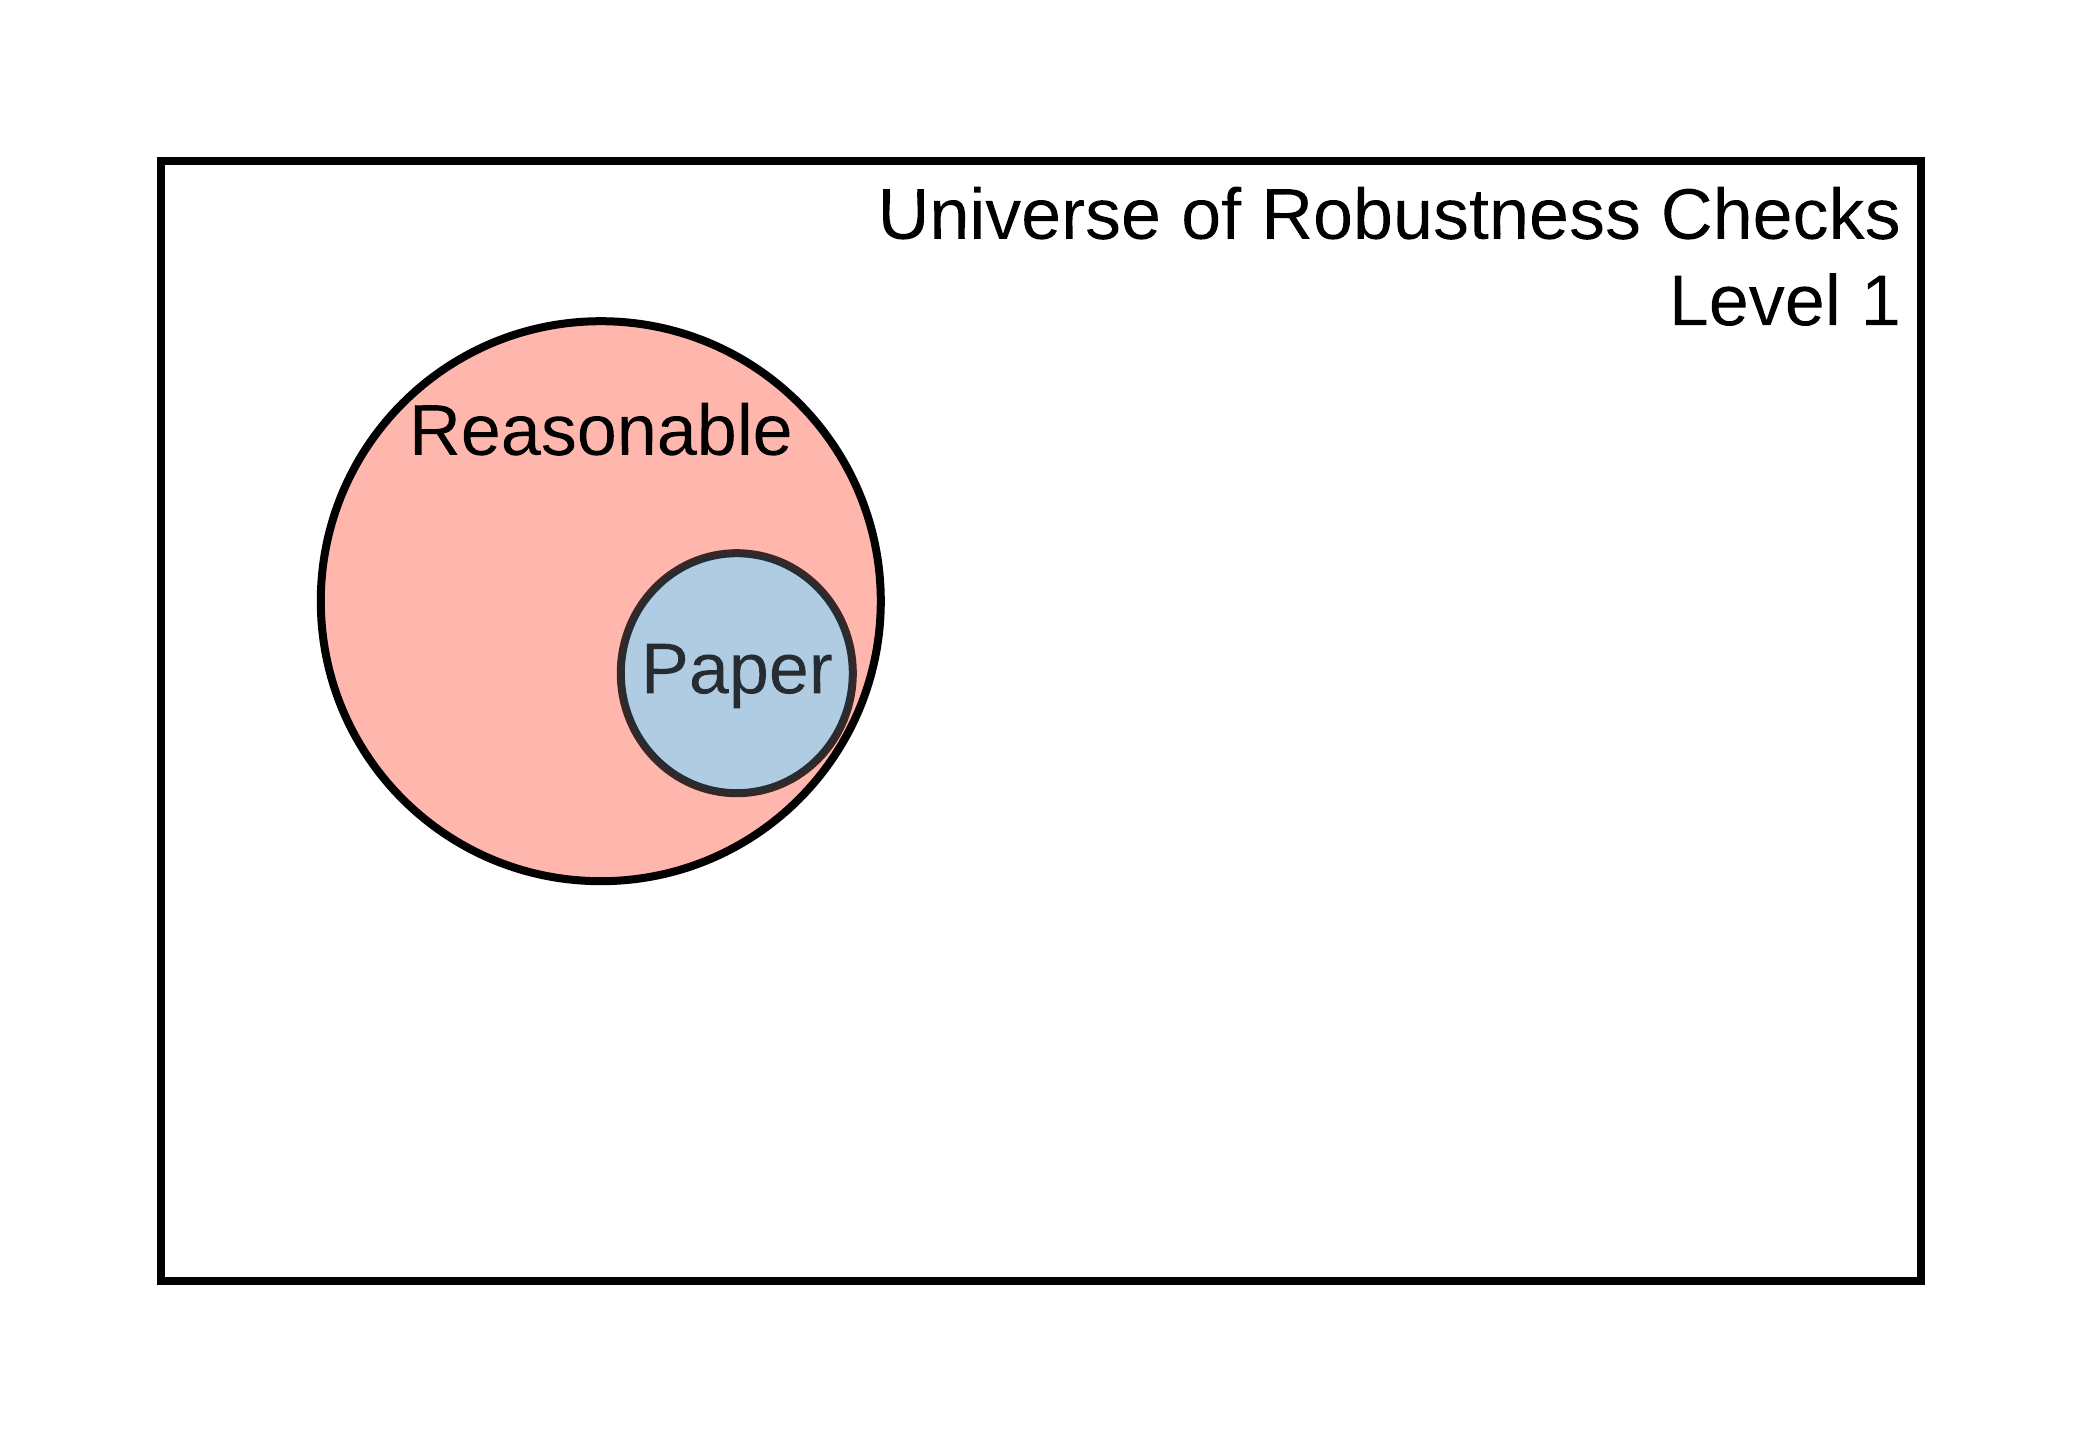
\includegraphics[width=0.5\linewidth]{images/robustness_lvl1} 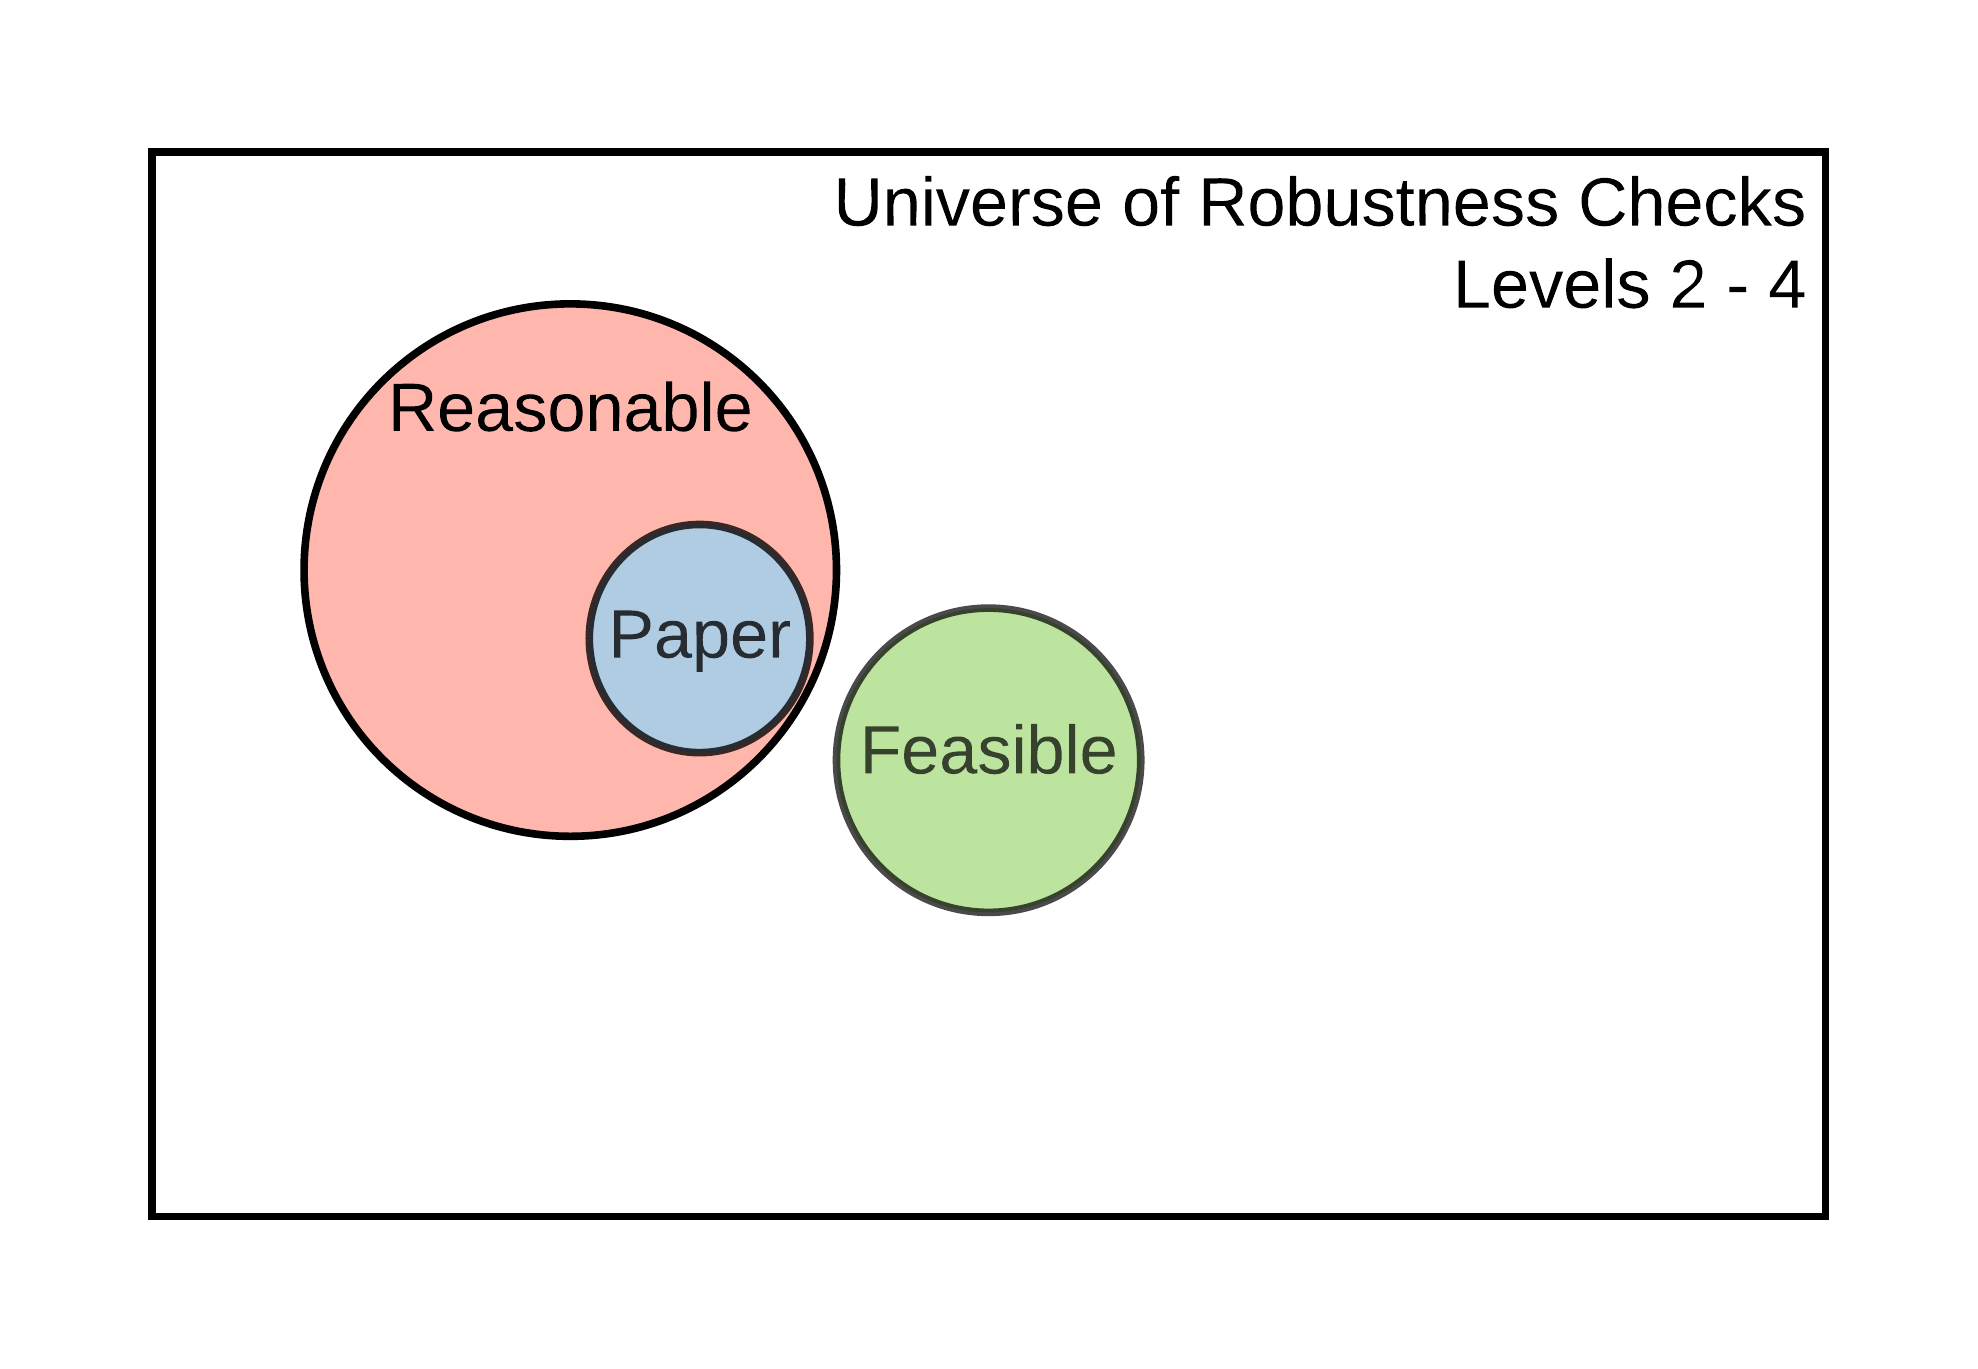
\includegraphics[width=0.5\linewidth]{images/robustness_lvl2_4} 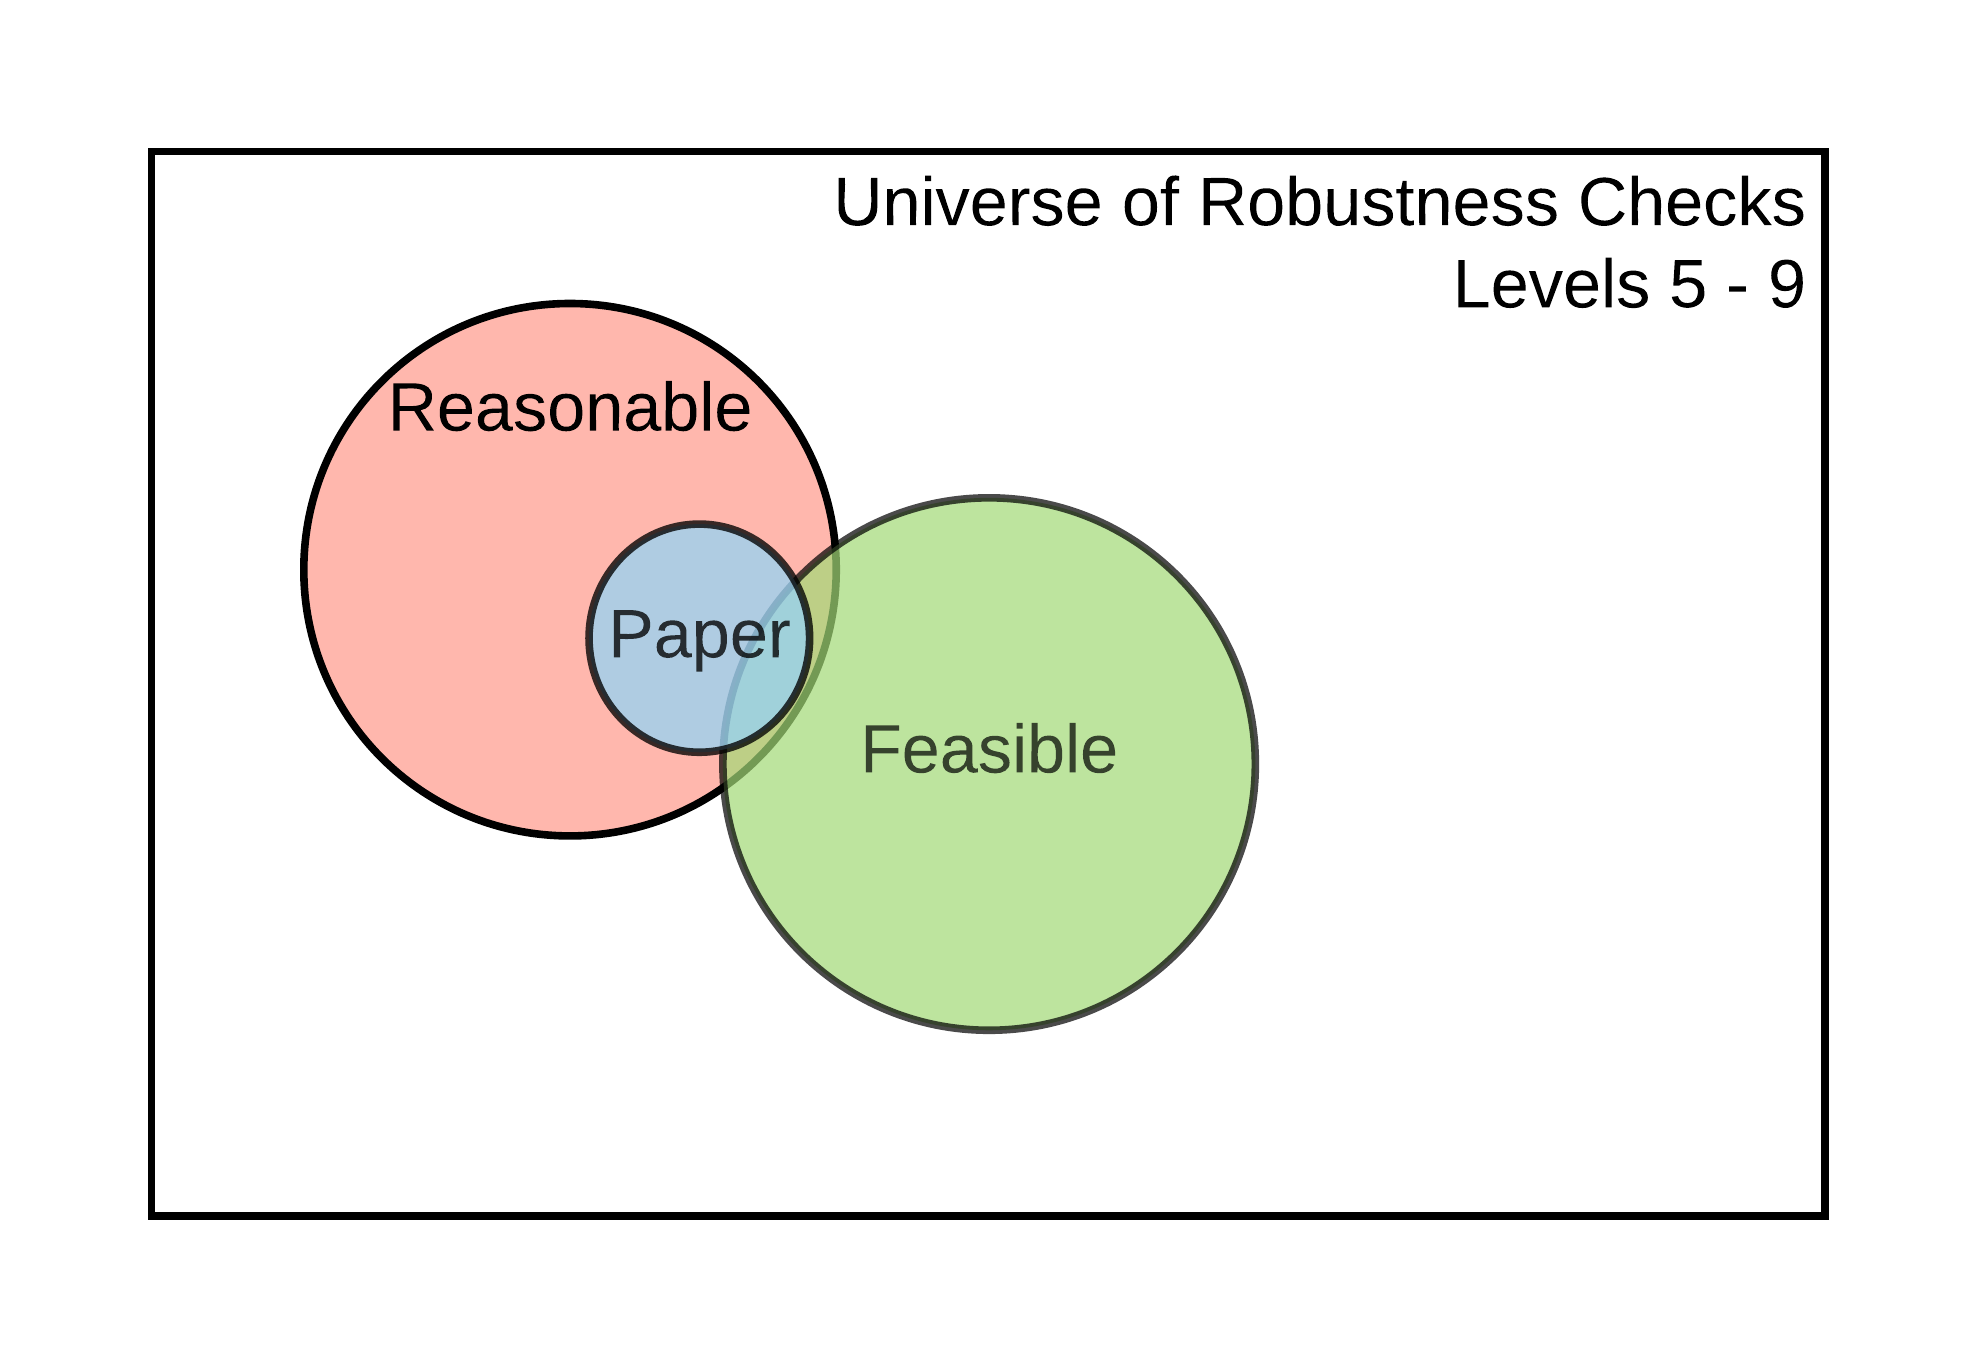
\includegraphics[width=0.5\linewidth]{images/robustness_lvl5-9} 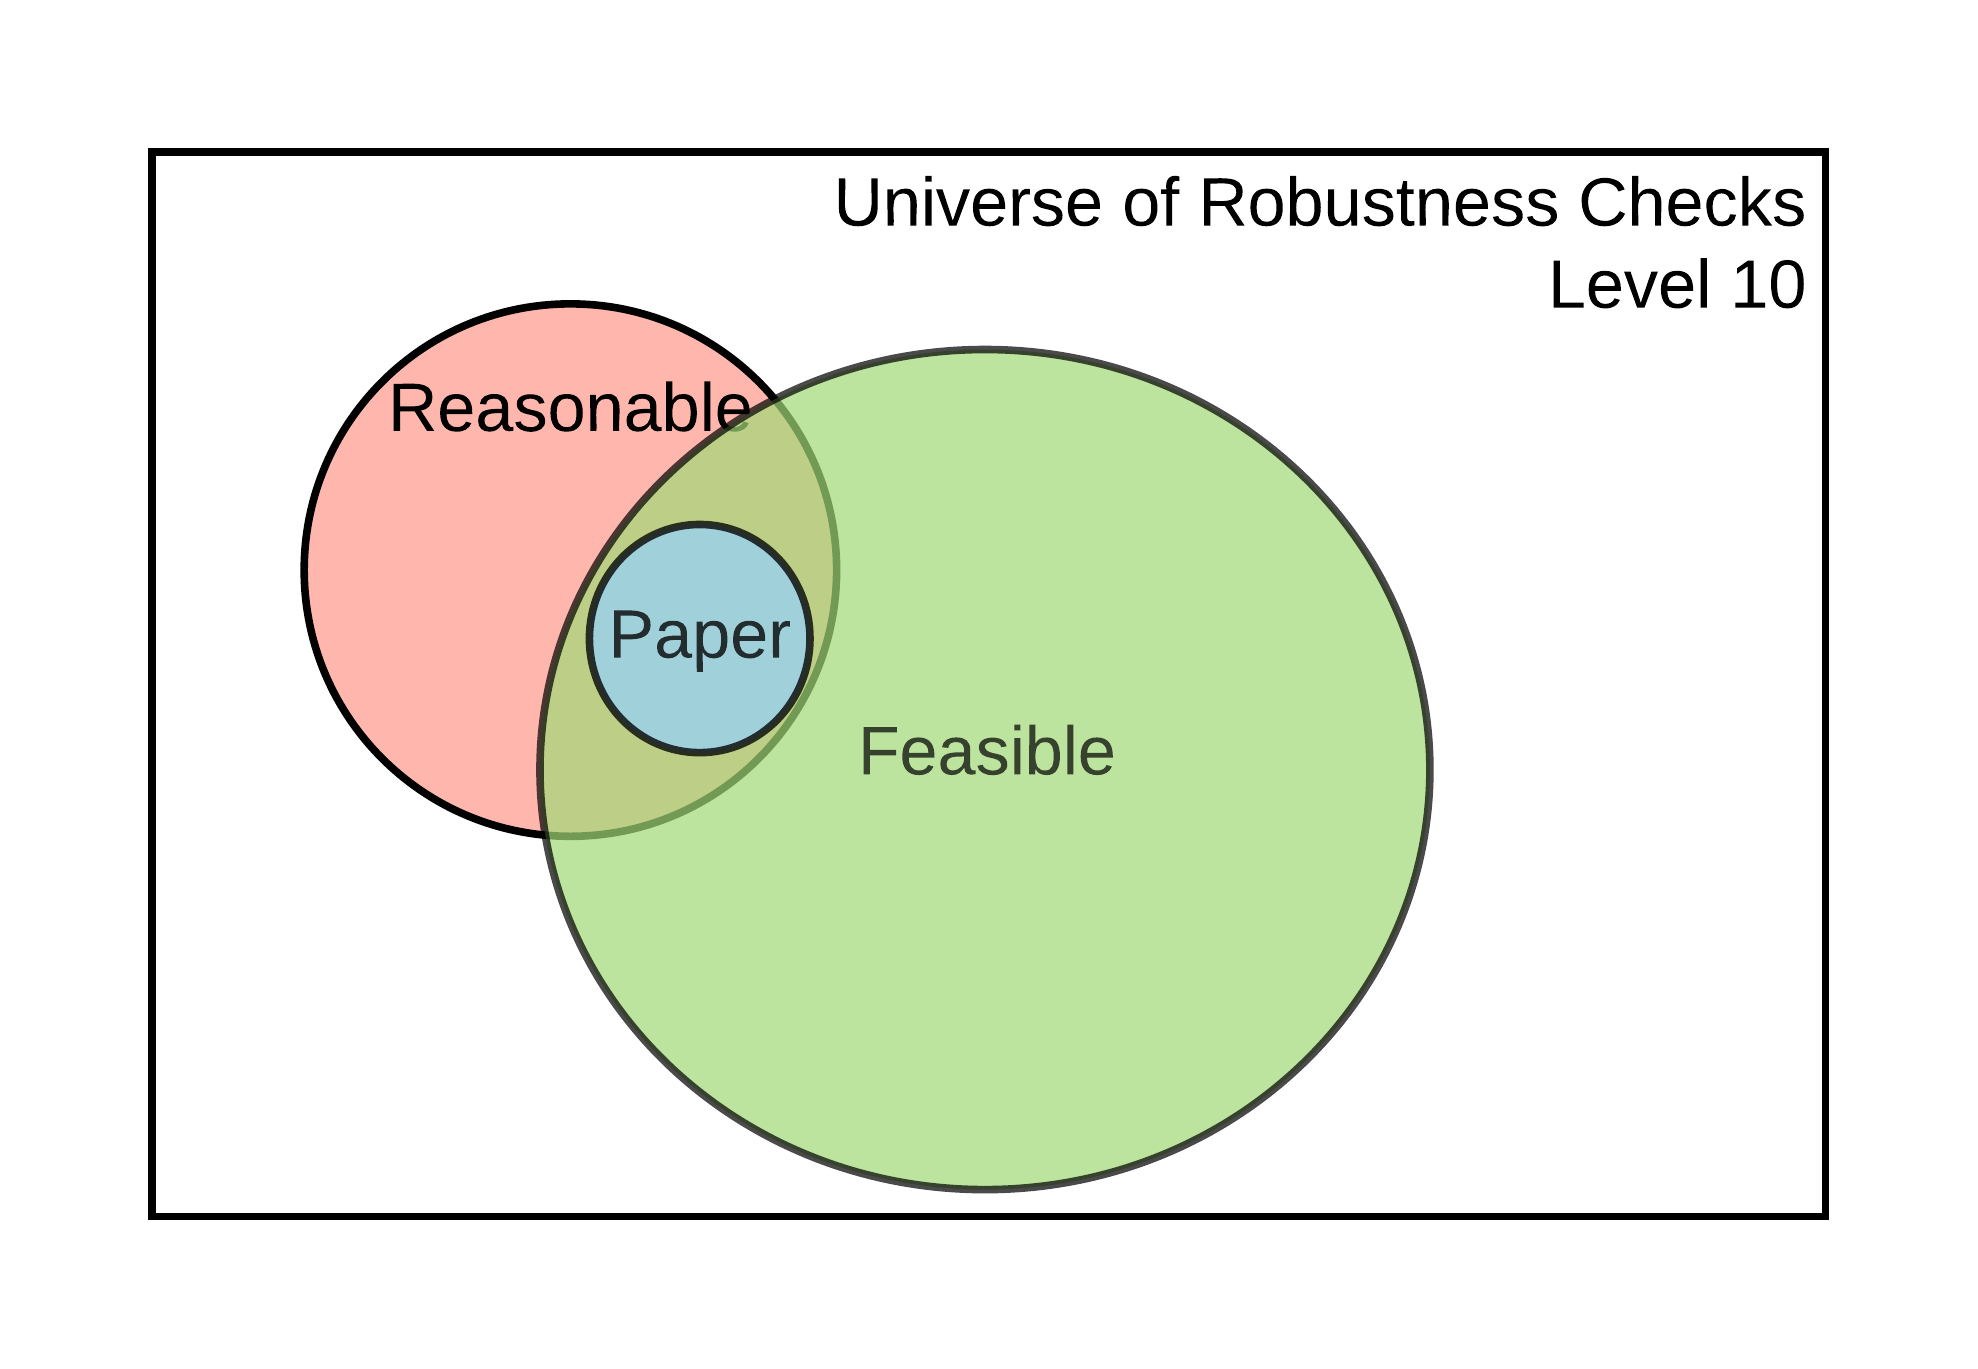
\includegraphics[width=0.5\linewidth]{images/robustness_lvl10} \caption{Universe of robustness tests and its elements}\label{fig:robusts}
\end{figure}

The size of the set of feasible robustness checks, and the likelihood that it contains reasonable specifications, will depend on the current level of reproducibility of the results that support a claim. The idea is illustrated in Figure \ref{fig:robusts}. At Levels 1-2, it is impossible to perform additional robustness checks because there are no data to work with. It may be possible to perform additional robustness checks for claims supported by display items reproducible at Levels 3-4, but not using the estimates declared in \emph{Scoping} (because the display items are not computationally reproducible from analysis data). It is possible to conduct additional robustness checks to validate the core conclusions of a claim based on a display item reproducible at Level 5. Finally, claims associated with display items reproducible at Level 6 or higher allow for robustness checks that involve variable definitions and other types of analytical choices.

The number of feasible robustness checks grows exponentially with improved reproducibility. For example, when checking the robustness of a new variable definition, you could test alternative variable definitions \emph{and} changes in the main estimate under an alternative variable definition.

Robustness is assessed at the claim level (see the diagram with a typical paper's components \ref{fig:stages-unit}). There may be several specifications presented in the paper for a given claim, one of which the authors (or you, if the authors did not indicate) have chosen as the main or preferred specification. Identify which display item contains this specification and refer to the reproduction tree to identify the code files in which you can modify a computational choice. Using the \protect\hyperlink{complete-tree}{example tree} discussed in the \emph{Assessment} stage, we can obtain the following (we removed the data files for simplicity). This simplified tree provides a list of potential files in which you can test different specifications:

\begin{verbatim}
        table1.tex (contains preferred specification of a given claim)
            |___[code] analysis.R
                    |___[code] final_merge.do
                            |___[code] clean_merged_1_2.do
                            |       |___[code] merge_1_2.do
                            |               |___[code] clean_raw_1.py
                            |               |___[code] clean_raw_2.py
                            |___[code] clean_merged_3_4.do
                                    |___[code] merge_3_4.do
                                            |___[code] clean_raw_3.py
                                            |___[code] clean_raw_4.py
\end{verbatim}

Here we suggest two types of contributions to robustness checks: (1) increasing the number of feasible robustness checks by identifying key analytical choices in code scripts and (2) justifying and testing reasonable specifications within the set of feasible checks. Both contributions should be recorded on the SSRP Platform and be linked to specific files in the reproduction package.

\hypertarget{feasible-robustness-checks-increasing-the-number-of-feasible-specifications}{%
\section{Feasible robustness checks: increasing the number of feasible specifications}\label{feasible-robustness-checks-increasing-the-number-of-feasible-specifications}}

Increasing the number of feasible robustness checks requires identifying the specific line(s) in the code scripts that execute an analytical choice. An advantage of this type of contribution is that you don't need to have an in-depth knowledge of the paper and its methodology to contribute. This allows you to potentially map several code files, achieve a broader understanding of the paper, and build on top of others' work. The disadvantage is that you are not expected to test and justify the reasonableness of alternative specifications.

Analytical choices can include those behind data cleaning and data analysis. Below are some proposed types for each category.

\textbf{Analytical choices in data cleaning code}

\begin{itemize}
\tightlist
\item
  Variable definition
\item
  Data sub-setting
\item
  Data re-shaping (merge, append, long/gather, wide/spread)
\item
  Others (specify as ``processing - other'')
\end{itemize}

\textbf{Analytical choices in analysis code}

\begin{itemize}
\tightlist
\item
  Regression function (link function)
\item
  Key parameters (tuning, tolerance parameters, and others)
\item
  Controls
\item
  Adjustment of standard errors
\item
  Choice of weights
\item
  Treatment of missing values
\item
  Imputations
\item
  Other (specify as ``methods - other'')
\end{itemize}

To record a specific analytical choice on the SSRP, please follow these steps:

\begin{enumerate}
\def\labelenumi{\arabic{enumi}.}
\item
  Review a specific code file (e.g.~\texttt{clean\_merged\_1\_2.do}) and identify an analytical choice (e.g.~\texttt{regress\ y\ x\ if\ gender\ ==\ 1}).
\item
  Record the file name, line number, reproduction package (original or name of revised version), choice type, and choice value. For the \texttt{source} field, type \emph{``original''} whenever the analytical choice is identified for the first time, and \texttt{line\ number} each time the same analytical choice is applied thereafter (for example, if an analytical choice is identified for the first time in line \#103 and for the second time in line \#122 their respective values for the \texttt{source} field should be \texttt{original} and \texttt{103}). For each analytical choice recorded, add the specific choice used in the paper and, optionally, describe what alternatives could have been used. The resulting database would look \href{https://docs.google.com/spreadsheets/d/1nZuJSHswbZgaaIfBcyIUGPwG-WIP8zE1Oambud-WoDc/edit?usp=sharing}{like this}:
\end{enumerate}

\begin{longtable}[]{@{}lllllll@{}}
\toprule
\begin{minipage}[b]{(\columnwidth - 6\tabcolsep) * \real{0.06}}\raggedright
entry\_id\strut
\end{minipage} & \begin{minipage}[b]{(\columnwidth - 6\tabcolsep) * \real{0.09}}\raggedright
file\_name\strut
\end{minipage} & \begin{minipage}[b]{(\columnwidth - 6\tabcolsep) * \real{0.09}}\raggedright
line\_number\strut
\end{minipage} & \begin{minipage}[b]{(\columnwidth - 6\tabcolsep) * \real{0.15}}\raggedright
choice\_type\strut
\end{minipage} & \begin{minipage}[b]{(\columnwidth - 6\tabcolsep) * \real{0.23}}\raggedright
choice\_value\strut
\end{minipage} & \begin{minipage}[b]{(\columnwidth - 6\tabcolsep) * \real{0.22}}\raggedright
choice\_range\strut
\end{minipage} & \begin{minipage}[b]{(\columnwidth - 6\tabcolsep) * \real{0.15}}\raggedright
Source\strut
\end{minipage}\tabularnewline
\midrule
\endhead
\begin{minipage}[t]{(\columnwidth - 6\tabcolsep) * \real{0.06}}\raggedright
1\strut
\end{minipage} & \begin{minipage}[t]{(\columnwidth - 6\tabcolsep) * \real{0.09}}\raggedright
code\_01.do\strut
\end{minipage} & \begin{minipage}[t]{(\columnwidth - 6\tabcolsep) * \real{0.09}}\raggedright
73\strut
\end{minipage} & \begin{minipage}[t]{(\columnwidth - 6\tabcolsep) * \real{0.15}}\raggedright
data sub-setting\strut
\end{minipage} & \begin{minipage}[t]{(\columnwidth - 6\tabcolsep) * \real{0.23}}\raggedright
males\strut
\end{minipage} & \begin{minipage}[t]{(\columnwidth - 6\tabcolsep) * \real{0.22}}\raggedright
males, female,\strut
\end{minipage} & \begin{minipage}[t]{(\columnwidth - 6\tabcolsep) * \real{0.15}}\raggedright
original\strut
\end{minipage}\tabularnewline
\begin{minipage}[t]{(\columnwidth - 6\tabcolsep) * \real{0.06}}\raggedright
2\strut
\end{minipage} & \begin{minipage}[t]{(\columnwidth - 6\tabcolsep) * \real{0.09}}\raggedright
code\_01.do\strut
\end{minipage} & \begin{minipage}[t]{(\columnwidth - 6\tabcolsep) * \real{0.09}}\raggedright
122\strut
\end{minipage} & \begin{minipage}[t]{(\columnwidth - 6\tabcolsep) * \real{0.15}}\raggedright
variable definition\strut
\end{minipage} & \begin{minipage}[t]{(\columnwidth - 6\tabcolsep) * \real{0.23}}\raggedright
income = wages + capital gains\strut
\end{minipage} & \begin{minipage}[t]{(\columnwidth - 6\tabcolsep) * \real{0.22}}\raggedright
wages, capital gains, gifts\strut
\end{minipage} & \begin{minipage}[t]{(\columnwidth - 6\tabcolsep) * \real{0.15}}\raggedright
``code\_01.do-L103''\strut
\end{minipage}\tabularnewline
\begin{minipage}[t]{(\columnwidth - 6\tabcolsep) * \real{0.06}}\raggedright
3\strut
\end{minipage} & \begin{minipage}[t]{(\columnwidth - 6\tabcolsep) * \real{0.09}}\raggedright
code\_05.R\strut
\end{minipage} & \begin{minipage}[t]{(\columnwidth - 6\tabcolsep) * \real{0.09}}\raggedright
143\strut
\end{minipage} & \begin{minipage}[t]{(\columnwidth - 6\tabcolsep) * \real{0.15}}\raggedright
controls\strut
\end{minipage} & \begin{minipage}[t]{(\columnwidth - 6\tabcolsep) * \real{0.23}}\raggedright
age, income, education\strut
\end{minipage} & \begin{minipage}[t]{(\columnwidth - 6\tabcolsep) * \real{0.22}}\raggedright
age, income, education, region\strut
\end{minipage} & \begin{minipage}[t]{(\columnwidth - 6\tabcolsep) * \real{0.15}}\raggedright
original\strut
\end{minipage}\tabularnewline
\begin{minipage}[t]{(\columnwidth - 6\tabcolsep) * \real{0.06}}\raggedright
\ldots{}\strut
\end{minipage} & \begin{minipage}[t]{(\columnwidth - 6\tabcolsep) * \real{0.09}}\raggedright
\ldots{}\strut
\end{minipage} & \begin{minipage}[t]{(\columnwidth - 6\tabcolsep) * \real{0.09}}\raggedright
\ldots{}\strut
\end{minipage} & \begin{minipage}[t]{(\columnwidth - 6\tabcolsep) * \real{0.15}}\raggedright
\ldots{}\strut
\end{minipage} & \begin{minipage}[t]{(\columnwidth - 6\tabcolsep) * \real{0.23}}\raggedright
\ldots{}\strut
\end{minipage} & \begin{minipage}[t]{(\columnwidth - 6\tabcolsep) * \real{0.22}}\raggedright
\ldots{}\strut
\end{minipage} & \begin{minipage}[t]{(\columnwidth - 6\tabcolsep) * \real{0.15}}\raggedright
\ldots{}\strut
\end{minipage}\tabularnewline
\bottomrule
\end{longtable}

\hypertarget{justifying-and-testing-reasonable-robustness-checks}{%
\section{Justifying and testing reasonable robustness checks}\label{justifying-and-testing-reasonable-robustness-checks}}

Justifying and testing a specific analytical choice involves identifying a feasible analytical choice, conducting a variation on it, and justifying its reasonableness. This approach's advantage is that it allows for an in-depth inspection of a specific section of the paper. Its main limitation is that justifying sensibility and validity (and non-redundancy, to an extent) requires a deeper understanding of the paper's topic and the methods. That may mean that undergraduate students or graduate students with only a surface-level interest in the paper (or limited time) may find it challenging to conduct this part of the reproduction.

When performing a specific robustness check, follow these steps:

\begin{enumerate}
\def\labelenumi{\arabic{enumi}.}
\item
  Eventually, you will be able to search the SSRP database of feasible robustness checks (discussed above) and record the identifier(s) corresponding to the analytical choice(s) of interest (\texttt{entry\_id}), but you can skip this for now. You can create an Entry ID by simply numbering the feasible specifications in the order as you record them.
\item
  Propose a specific variation to this analytical choice.
\item
  Discuss whether you think this variation is sensible, specifically in the context of the claim tested (e.g., does it make sense to include or exclude low-income Hispanic people from the sample when assessing the impact of a large wave of new immigrants?).
\item
  Discuss how this variation could affect the validity of the results (e.g., likely effects on the omitted variable bias, measurement error, change in the Local Average Treatment Effects for the underlying population).
\item
  Confirm that test is not redundant with other tests in the paper or the robustness exercise.
\item
  Report the result of the robustness check (new estimate, standard error, and units).
\end{enumerate}

\hypertarget{concluding-the-reproduction}{%
\chapter{Concluding the Reproduction}\label{concluding-the-reproduction}}

Once you have completed each of the reproduction stages for all of your claims of interest, you will be ready to submit your work. For a reproduction to be considered complete and ready for submission, you must have \textbf{assessed at least one display item.}

Before submitting a reproduction, you will be able to modify your answers to any entry in the ACRE platform. After you hit ``Submit'', however, you will not be able to modify your reproduction attempt any further. If you wish to modify your reproduction after submitting it, you will have to record \emph{a new reproduction attempt} on the platform and link to the previously completed reproduction. \textbf{Tip:} the platform allows to clone entire reproductions up to the scoping stage. If you also want to bring in content from some of the labor-intensive parts in later stages (describing all the inputs, documenting analytical choices) you can download the csv file of previous forms and upload them to a new reproduction.

\hypertarget{outputs}{%
\section{Outputs}\label{outputs}}

A completed reproduction will consist of three different types of outputs:

\textbf{1. Revised reproduction package} -- Deposit your revised version of the original reproduction package in a trusted repository, such as \href{https://dataverse.org/}{Dataverse}, \href{https://www.openicpsr.org/openicpsr/}{openICPSR}, \href{https://figshare.com}{Figshare}, \href{https://datadryad.org/stash}{Dryad}, \href{https://about.zenodo.org/}{Zenodo}, or the \href{osf.io/}{Open Science Framework}. You should submit a revised reproduction package any time that you perform any type of \protect\hyperlink{improvements}{improvement} to the original reproduction package. This revised reproduction package is expected to be self-contained as it might be used by future reproducers for assessment and improvement. If your new reproduction package is larger than the capacity of your trusted repository (around 2GB), or it contains data that you do not have permission to share, remove the specific files from your reproduction package and add a reference to the original reproduction package. For example if your reproduction package contains a file that cannot be shared, locate leave a note in the readme file with its relative location (e.g.~\texttt{/data/large\_confidential\_file.csv}) and specific instructions on how to obtain it.

Before submitting the reproduction, make sure that your revised reproduction package fulfills the following requirements:

\begin{itemize}
\tightlist
\item
  Has a digital object identifier (DOI). All of the trusted repositories referenced above generate DOIs. This is a stable, citable link that will allow others to easily find your work.
\item
  Is titled following this convention: \texttt{revised\ reproduction\ package\ for\ -\ title\ of\ the\ paper\ -\ last\ name\ of\ reproducer\ -\ year\ when\ the\ reproduction\ was\ completed}
\item
  If it is not self-contained, indicate the DOI of the last reproduction package used for the reproduction (the original or a previously revised reproduction package), and the relative file location of the missing files (e.g.~\texttt{/data/raw/large\_file.csv}).
\end{itemize}

\textbf{2. Reproduction report(s)} -- At the end of each stage, the Social Science Reproduction Platform will give you the option to generate a report summarizing your work for that stage. Once you've submitted your final reproduction, the platform will also automatically generate a final report with its own DOI (different from the DOI used for the revised reproduction package). If you are conducting this reproduction as part of a supervised course or project, your instructor or advisor should have defined the structure of those reports (e.g., Stage 1 and 2 reports may be part of problem set 1, and Stage 3 and 4 reports may be a part of problem set 2). Each report will contain the following information:

\begin{itemize}
\tightlist
\item
  \textbf{\emph{Scoping Report:}} basic information about the paper, descriptive statistics about the number of claims identified and the subset that was assessed, and a summary of the claims and associated specifications.\\
\item
  \textbf{\emph{Assessment Report:}} a summary of the display items assessed and their connections with the claims.\\
\item
  \textbf{\emph{Improvement Report:}} descriptions of improvements implemented and of improvements suggested for future reproductions, and an updated reproducibility score, if any.\\
\item
  \textbf{\emph{Robustness Report:}} summary of all of the analytical choices identified, and a description of the results of robustness tests to reasonable new specifications, if any.\\
\item
  \textbf{Final reproduction report:}* includes everything, plus final comments, and it cannot be edited after submission.
\end{itemize}

\textbf{3. Your data} -- You will be able to export several .csv files containing all of your table-form responses recorded as part of your reproduction attempt.

\hypertarget{visibility-and-data-use}{%
\section{Visibility and data use}\label{visibility-and-data-use}}

Before submitting your reproduction, we ask that you select one of three privacy models that determine what parts of your reproduction will be visible to other SSRP users upon publishing. We recommend using the \emph{public, identified} model, which allows other users to see the entirety of your reproduction and credits you directly as its author. However, you may choose to publish your reproduction \emph{anonymously} under either the \emph{class anonymous} or \emph{temporary anonymous} models, where other SSRP users can access unidentifiable data from your reproduction (e.g., numerical and categorical responses), but not your identity and identifiable data (free-form narrative answers such as notes, descriptions, summaries, and explanations). Please refer to the \href{https://www.socialsciencereproduction.org/terms-of-use}{Terms of Use} to learn more about each privacy model; however, here they are in a nutshell:

\begin{enumerate}
\def\labelenumi{\arabic{enumi}.}
\item
  \textbf{Public, identified:} this is the default privacy setting. You are listed as the reproduction's author, and other users can see the entire reproduction.
\item
  \textbf{Class anonymous:} allows you to conceal your identity and free-form narrative answers (notes, descriptions, summaries, explanations) indefinitely if you conducted the reproduction as part of a class, project, or some other assignment for credit at the university/post-secondary level. Other users can see basic class identifiers (course name, year, institution university, instructor's name, and email address) and categorical responses.
\item
  \textbf{Temporary anonymous:} allows you to embargo your identity and free-form narrative answers for up to 4 years after submitting. Requires an annually recurring opt-out to maintain the embargo. At the expiration of the embargo period or if you fail to opt-out, privacy settings are updated to ``public, identified''.
\end{enumerate}

The Social Science Reproduction Platform will aggregate descriptive statistics from all submitted reproductions recorded to produce reproducibility metrics across disciplines, sub-disciplines, journals, and topical bodies of literature. If you choose to remain anonymous and are not a student using the SSRP as part of a course, your work may still be integrated into these descriptive statistics.

\hypertarget{guidance-for-instructors-supervising-reproduction-assignments}{%
\chapter{Guidance for Instructors Supervising Reproduction Assignments}\label{guidance-for-instructors-supervising-reproduction-assignments}}

The \href{https://www.socialsciencereproduction.org/}{Social Science Reproduction Platform} (SSRP) is an open-source platform that crowdsources and catalogs attempts to assess and improve the computational reproducibility of published social science research. Instructors can use the SSRP in combination with this Guide (called the ``ACRe Guide'') to facilitate reproduction assignments (sometimes called ``replications'') in applied social science courses at the graduate and undergraduate levels. Students can use these materials with little to no supervision, covering the following learning activities:

\begin{itemize}
\tightlist
\item
  Assessing and improving the reproducibility of published work\\
\item
  Applying good coding and data management practices\\
\item
  Recording reproduction results and improvements on the SSRP\\
\item
  Engaging in constructive exchanges with authors\\
\item
  Developing a deep understanding of common methods and computational techniques\\
\item
  Creating real, citable scientific contributions.
\end{itemize}

In the process, students can reference the ACRe Guide as a step-by-step protocol for conducting reproductions and use the SSRP to record and share their work, and instructors can use it as a guide for supervising these assignments. Examples of completed reproductions are available \href{https://www.socialsciencereproduction.org/reproductions/search?query=}{here}.

Reproductions typically include five distinct stages (elaborated on at length in the chapters of this Guide):\\
1. \emph{\href{https://bitss.github.io/ACRE/select.html\#select}{Paper selection}}, where students select a paper and try to locate its reproduction package;\\
2. \emph{\href{https://bitss.github.io/ACRE/scoping.html\#scoping}{Scoping}}, where students define the scope of the reproduction by recording the claims, display items, and specifications to focus on;\\
3. \emph{\href{https://bitss.github.io/ACRE/assessment.html\#assessment}{Assessment}}, where students review and describe in detail the reproduction package, if available, and assess the current level of computational reproducibility of the selected display items;\\
4. \emph{\href{https://bitss.github.io/ACRE/improvements.html\#improvements}{Improvement}}, where students modify the content and/or the organization of the reproduction package to improve its reproducibility; and\\
5. \emph{\href{https://bitss.github.io/ACRE/robust.html\#robust}{Robustness}}, where students identify feasible robustness checks and/or assess the reasonableness of variations in analytical choices.

This chapter includes tips and resources for instructors interested in using the SSRP to teach reproducibility. We first identify typical use cases and suggest timelines for planning assignments. We then provide sample grading strategies and guidance in instances where the students would like to remain anonymous but still share their work on the SSRP.

\emph{Get started by \href{https://www.socialsciencereproduction.org/users/sign_in}{signing up for a free SSRP account} and reviewing this chapter to find tips based on your use case below.}

\hypertarget{common-use-cases}{%
\section{Common use cases}\label{common-use-cases}}

\hypertarget{graduate-level-assignment}{%
\subsection{Graduate-level assignment}\label{graduate-level-assignment}}

\emph{(Estimated duration: 2 weeks to one semester)}

Advanced master's or PhD-level courses often feature assignments where students reproduce published papers to gain familiarity with fundamental concepts, research methods, and applications. In these courses, instructors can recommend students choose papers from specific sub-fields (e.g., labor economics) or journals, or curate a list of possible papers.

The length of such assignments can vary from a couple of weeks to a semester. For shorter timelines, instructors can ask students to conduct reproductions using only analysis data, focusing on just the main results. For longer timelines, such as semester-long assignments, students might reproduce entire papers from raw data. See section 7.2 below for a suggested distribution of effort across different lengths of assignments.

Graduate students should expect to spend a significant time at the \emph{Robustness} stage. Therefore, before beginning the assignment, we recommend that students focus either on expanding the set of feasible robustness checks (see \href{https://bitss.github.io/ACRE/robust.html}{Chapter 5}) or on testing and defending the reasonableness of a specific robustness check (which may contain more variations in more than one analytical choice).

\hypertarget{undergraduate-thesis}{%
\subsection{Undergraduate thesis}\label{undergraduate-thesis}}

\emph{(Estimated duration: 2 months to 1 year)}

Students can use the platform to carry out detailed reproductions as part of an undergraduate thesis (see an example \href{https://osf.io/3e6ps/}{here}). This type of assignment allows students to gain direct research experience while making meaningful contributions to the field.

Depending on the paper's scope and the assignment's learning objectives, such projects could last anywhere from a couple of months to an entire year. Students should demonstrate an understanding of the paper by identifying its main claim(s) at the \emph{Scoping} stage and conducting a detailed assessment of the reproducibility of their associated display items at the Assessment stage. At the \emph{Improvement} stage, students should try to improve the reproducibility of at least one display item. Depending on the scope of the paper, examples within reach of an undergraduate thesis might include finding and cleaning the raw data, translating code scripts into a different programming language (ideally open source), using dynamic documents, or making other improvements suggested by the instructor. Finally, at the \emph{Robustness} stage, students should be able to demonstrate a high-level understanding of the conditions under which the paper's estimates are valid.

We recommend breaking down the assignment into a ``proposal'' stage, where students scope and assess their papers, and an ``execution'' stage, where students carry out improvements and robustness checks.

\hypertarget{undergraduate-course}{%
\subsection{Undergraduate course}\label{undergraduate-course}}

\emph{(Estimated duration: 1 month to one semester)}

Students in undergraduate courses should primarily focus on verifying whether reproductions packages ``run'' and recording the outcome on the SSRP. At the \emph{Scoping} stage, undergraduate students can demonstrate a high-level understanding of the paper's main claims. Students can identify the code and files necessary to reproduce their select display items at the \emph{Assessment} stage and try to actually run the code. Finally, at the \emph{Robustness} stage students can inspect the code scripts and identify potential lines of code with analytical choices, increasing the feasible set of robustness checks.

\hypertarget{paper-selection-and-assignment-timelines}{%
\section{Paper selection and assignment timelines}\label{paper-selection-and-assignment-timelines}}

The SSRP allows for flexibility in selecting papers and determining the scope of reproduction assignments in terms of the number of claims, display items, or even the required reproduction stages (at minimum, a complete reproduction requires filling in \emph{Scoping} and \emph{Assessment}). For example, instructors can \textbf{curate a list of target papers} or \textbf{allow students to choose} from a distinct body of literature or a specific journal. For either strategy, a good starting point is first to reference the \href{https://www.socialsciencereproduction.org/reproductions/search}{SSRP database of papers and reproductions}, which allows users to search through submitted reproductions. This can help detect potential ``no-go'' papers for which other users were unable to find any reproduction materials (labeled as ``abandoned papers''), though users are by no means barred from attempting to reproduce such cases. If instructors are unable to curate a list of papers with readily available reproduction packages, we recommend allocating at least 3 additional weeks to try to locate the missing reproduction materials, potentially by contacting the original authors (see \href{https://bitss.github.io/ACRE/comunications.html\#comunications}{this chapter} for guidance on constructive exchanges with original authors).

To curate a list of target papers in \emph{economics}, instructors can consult recently published articles in the journals of the \href{https://www.aeaweb.org/journals}{American Economic Association} (AEA), especially articles published since 2019, which are more likely to contain reproduction packages given a change in the \href{https://www.aeaweb.org/journals/data/data-code-policy}{AEA Data and Code Availability Policy} that took effect that year. In \emph{political science}, target papers can be found in the \emph{\href{https://ajps.org/ajps-verification-policy/}{American Journal of Political Science}}, especially those published after 2016, which are also likely to contain reproduction packages. In other social science disciplines, instructors can focus on journals that score 2 or above in data, code, and materials transparency in the \href{https://www.cos.io/initiatives/top-guidelines}{Transparency and Openness Promotion (TOP) Factor} (see scores \href{https://topfactor.org/}{here}), maintained by the Center for Open Science.

To plan the distribution of effort across different reproduction stages, we recommend consulting Table 1 below. The \emph{Scoping} and \emph{Assessment} stages will take approximately the same amount of time across timelines, but will depend on the students' prior experience with reproductions and the SSRP. Larger differences emerge in the distribution of time for the last two main stages: Improvements and Robustness. For shorter exercises, we recommend avoiding any possible improvements to the raw data (or cleaning code), which may limit the number of possible robustness checks.

\textbf{Table 1: Workload distribution across reproduction stages across different timelines}

2 weeks (\textasciitilde10 days)

1 month (\textasciitilde20 days)

1 semester (\textasciitilde100 days)

analysis data

raw data

analysis data

raw data

analysis data

raw data

Scoping

10\% (1 day)

5\% (1 day)

5\% (5 days)

Assessment

35\%

25\%

15\%

Improvement

25\%

0\%

40\%

30\%

20\%

Robustness

25\%

5\%

30\%

30\%

\hypertarget{grading-strategy}{%
\section{Grading strategy}\label{grading-strategy}}

Once students have completed their reproductions, they can generate and share with instructors links to view-only reports of their work. Instructors can use these reports to grade and provide feedback on students' work. Below we suggest a strategy for grading based on the use cases described above. For assignments that don't contain all reproduction stages, we recommend distributing credits proportionally to the stages that were filled out.

We suggest the following grading categories:

\begin{itemize}
\tightlist
\item
  \textbf{Submission:} Full credit for timely submitted, non-blank submissions.\\
\item
  \textbf{All key fields:} Full credit for filling out details such as paper information, reproduction package links, claims summary for at least one claim, table with claims estimates, inputs description, display item assessments (particularly the subjective assessment section), and assessment of paper-level reproducibility.\\
\item
  \textbf{Paper summary:} Full credit for submitting a short summary of the paper that answers \href{https://bitss.github.io/ACRE/scoping.html\#read-sum}{these questions}.\\
\item
  \textbf{Claims:} Full credit for presenting an accurate and clear summary of the paper's main claims (see guidance \href{https://bitss.github.io/ACRE/scoping.html\#scoping}{here}). To properly score this section, the instructor needs to have previous knowledge of the paper.\\
\item
  \textbf{Assessment:} There are two kinds of contributions students can make to obtain full credit:

  \begin{itemize}
  \tightlist
  \item
    Assess \emph{multiple claims}. Additional credit per each assessment could be assigned at a decreasing rate (e.g., in addition to the first assessment scored in ``All key fields'' give 50\% of the credit for assessing a second claim, 30\% for a third, and 20\% for a fourth).\\
  \item
    Conduct a \emph{thorough assessment of a single claim}. This can be done by clearly identifying all of the inputs (data sources, analysis data, and code scripts) and providing detailed documentation of the reproduction attempt (e.g., duration of execution, errors detected, specific missing files, details about the required computational environment).\\
  \end{itemize}
\item
  \textbf{Improvement:} Students can obtain full credit through two types of contributions:

  \begin{itemize}
  \tightlist
  \item
    Implement improvements of reproducibility of \emph{multiple claims} with a similar credit structure as for the assessment of multiple claims (see point above).\\
  \item
    Implement \emph{thorough improvements of a single claim}. The Improvements chapter describes several types of possible improvements. A key requirement is that students clearly document their improvements (see \href{https://bitss.github.io/ACRE/improvements.html\#doc-impr}{this section} for suggestions on how to do this).\\
  \end{itemize}
\item
  \textbf{Future suggestions for improvement:} Instructors can also assign credit for specific suggestions for improvements recorded for future reproducers to attempt. Full credit should be assigned when the recommendations are concrete, feasible, and demonstrate that the student performed an in-depth review of the code and data.\\
\item
  \textbf{Revised reproduction package:} Full credit for students who post a revised reproduction package in a trusted repository. Instructors can verify its existence by clicking on the link provided on the reproduction summary page. If the student used version control software as part of the revised reproduction package, the instructor can easily verify the modifications relative to the original reproduction package by checking the commits history.\\
\item
  \textbf{Robustness:} Students can obtain full credit for one of two strategies (or a combination of them):

  \begin{itemize}
  \tightlist
  \item
    Identify a large number of original analytical choices in the code files. The definition of ``large'' is up to the Instructor, but we suggest at least 20 original analytical choices (see \href{https://bitss.github.io/ACRE/robust.html\#robust}{this section} for a distinction between original and non-original analytical choices).\\
  \item
    Conduct a robustness test by modifying one or more analytical choices identified in the paper. Full credit is assigned for a clear and accurate discussion of the results and their reasonableness.
  \end{itemize}
\end{itemize}

\begin{longtable}[]{@{}lcc@{}}
\toprule
& Score (example) & Weights (suggested)\tabularnewline
\midrule
\endhead
Submitted & 100 & 40\%\tabularnewline
All important fields & 80 & 10\%\tabularnewline
Summary & 100 & 5\%\tabularnewline
Clear claims & 90 & 5\%\tabularnewline
Assessment & 100 & 10\%\tabularnewline
Improvements & 50 & 10\%\tabularnewline
Revise reproduction package & 100 & 5\%\tabularnewline
Specific suggestions for improvements & 0 & 5\%\tabularnewline
Robustness & 100 & 10\%\tabularnewline
Final Score & 87.5 &\tabularnewline
\bottomrule
\end{longtable}

\hypertarget{facilitating-class-anonymous-reproductions}{%
\section{\texorpdfstring{Facilitating \emph{class anonymous} reproductions}{Facilitating class anonymous reproductions}}\label{facilitating-class-anonymous-reproductions}}

The SSRP allows users to select from three distinct privacy models when submitting their work, including \emph{public-identified}, \emph{temporary anonymous}, and \emph{class anonymous} (explained in more detail \href{https://bitss.github.io/ACRE/concluding-the-reproduction.html\#visibility-and-data-use}{here}). This section includes specific guidance for instructors facilitating reproductions that will be published using the \emph{class anonymous} privacy model, which allows users to conceal their identities and free-form narrative answers (e.g., notes, descriptions, summaries, explanations) indefinitely. Instead, reproductions published under the class anonymous model contain only categorical responses and basic class identifiers, including course name, year, institution, instructor's name, and instructor's email address.

Reproducers looking to publish under the \emph{class anonymous} model will be unable to maintain their anonymity if they share their revised reproduction packages as part of their reproductions. This is because trusted data repositories and GitHub require users to create accounts in order to post their content and keep records of updates. We advise instructors to create generic repositories for their class (e.g., ``Reproductions for Econ 270 - Fall 2021'') and deposit each anonymous reproduction in self-contained folders.

For example, suppose a class has two students who choose the anonymous option. In that case, they should share (privately) their revised reproduction package with their instructor, and the instructor should post them using the following structure:

\begin{Shaded}
\begin{Highlighting}[]
\NormalTok{  Reproductions for }\CommentTok{[}\OtherTok{Course Name, Semester}\CommentTok{]}
\NormalTok{    └── Revised reproduction package for Smith et al. (2019)}
\NormalTok{    └── Revised reproduction package for Perez et al. (2019)}
\end{Highlighting}
\end{Shaded}

\textbf{Note:} When anonymizing revised reproduction packages, we advise that instructors and students avoid using version control software. Even if the current materials are correctly de-identified, the version history may still contain identifiers, such as GitHub usernames.

\hypertarget{comunications}{%
\chapter{Guidance for Constructive Communication Between Reproducers and Original Authors}\label{comunications}}

This chapter contains guidance for constructive and respectful communication between reproducers and original authors. Exchanges that contain charged or adversarial language can damage professional relationships and hamper scientific progress. Janz and Freese (\href{https://www.mzes.uni-mannheim.de/openscience/wp-content/uploads/2019/01/Janz-Freese_-Good-and-Bad-Replications-1.pdf}{2019}) articulate two important steps reproducers can take to ensure that their interactions with original authors are constructive. We summarize and build on this approach below and encourage you to follow this guidance. Remember the \textbf{golden rule of reproductions} (and replications): \emph{treat others and their work, as you would like others to treat you and your work!}

\textbf{1. Carefully and transparently plan your study.}

\begin{enumerate}
\def\labelenumi{\alph{enumi}.}
\tightlist
\item
  Clearly state that you are conducting a reproduction of their original work.\\
\item
  Explain why you have chosen this study.
\item
  If you are not able to reproduce the results explain how ``far'' your results must deviate from the original work before claiming that the study could not be reproduced. Engage deeply with the substantive literature to ensure that your interpretation of differences between the original and reproduction is thorough and acceptable to other authors in the field.
\end{enumerate}

\textbf{2. Use professional and sensitive language. Discuss potential discrepancies between your work and the original paper, just like you might do for your own work.}

\begin{enumerate}
\def\labelenumi{\alph{enumi}.}
\tightlist
\item
  Avoid binary judgments and statements like ``failed to reproduce.'' Instead, state clearly which results reproduced and which did not (e.g., ``we successfully reproduced X, but failed to reproduce Y'') unless you uncover apparent scientific misconduct (e.g., see \href{https://doi.org/10.31222/osf.io/qy2se}{Broockman, Kalla and Aronow, 2015}).\\
\item
  Talk about \emph{the study, not the author} to avoid making it personal. Make clear what the positive contribution of the original article is. Consider sending a copy of your reproduction report to the original authors.\\
\item
  Discuss what your reproduction contributes to the literature, and refrain from claiming to give the final answer to the question.\\
\item
  For papers published five or more years ago, be mindful that norms for reproducibility have evolved since then.\\
\item
  Remember, \emph{the goal is not to criticize previous work or hunt for errors, but to move the literature forward!}
\end{enumerate}

To help you put these recommendations into practice, we developed template language for common scenarios that reproducers and authors may encounter in their interactions. While we hope you find these useful, note that they are \emph{only recommendations}, and you are welcome to modify them based on your project's context and needs. Feel free to \href{mailto:acre@berkeley.edu}{contact us} if you need more guidance or would like to provide feedback on these materials.

\hypertarget{for-reproducers-contacting-the-authors-of-the-original-study}{%
\section{For reproducers contacting the authors of the original study}\label{for-reproducers-contacting-the-authors-of-the-original-study}}

Consider the following \emph{before} you contact the original authors:

\begin{enumerate}
\def\labelenumi{\arabic{enumi}.}
\item
  Search the SSRP for reproduction materials or records of past interactions with the authors of a given paper. For each reproduction, consult the ``Author inquiries'' column to see whether authors have indicated whether they are available for further inquiries.
\item
  Carefully read all footnotes, appendices, tables, captions, etc., to learn if, how, and where reproduction materials are provided. Follow this \href{https://social-science-data-editors.github.io/guidance/Verification_guidance.html}{Data and Code Guidance} to determine whether you have everything before you start. A few things to consider:

  \begin{itemize}
  \tightlist
  \item
    A \emph{Readme} file, if available, would be a good place to start.\\
  \item
    Check whether there are any restrictions on accessing the data or code, and whether there are instructions on how to access these files for the purpose of reproduction.
  \end{itemize}
\item
  If a reproduction package is not readily available in the location where the article is published (e.g., the journal website), check the authors' websites, Dataverse profiles, or other relevant archives and/or data repositories like the \href{https://www.icpsr.umich.edu/icpsrweb/}{ICPSR Publications Related Archive}.
\item
  If steps 1 and 2 don't yield anything, contact the corresponding author (copying the co-authors, if any), consolidating your requests into as few emails as possible. In your email, make sure to include the following details:

  \begin{itemize}
  \tightlist
  \item
    Basic information about the paper to reproduce (include title, version, date, and a DOI (or just a URL));\\
  \item
    Context for the reproduction (as part of a class exercise, thesis, personal project, etc.) and a note that the outcome will be recorded on the \href{https://www.socialsciencereproduction.org/}{Social Science Reproduction Platform}(SSRP);
  \item
    Items from the reproduction package that are missing, as well as locations where you had (unsuccessfully) searched for them;\\
  \item
    Your use plan: Will the materials be used exclusively for this project? Ask for permission to share the data publicly.\\
  \item
    Right to consultation and results: Will you share the outcome of the reproduction with the original authors?\\
  \item
    A deadline to respond (we suggest at least two weeks).
  \end{itemize}
\item
  Follow up if you don't get a response within two weeks (or whatever deadline you set), and include any details or clarifications that were left out in your first email.
\item
  Record the outcome of your interaction with the original author at the \emph{Select a Paper} stage on the SSRP. You can qualify the outcome as one of the following:

  \begin{itemize}
  \tightlist
  \item
    A \emph{complete} reproduction package was provided;
  \item
    An \emph{incomplete} reproduction package was provided. You can also select one of the following reasons:

    \begin{itemize}
    \tightlist
    \item
      Data is of sensitive, confidential, or proprietary character and cannot be shared;
    \item
      Data is of sensitive, confidential, or proprietary character, but access instructions were provided.
    \end{itemize}
  \item
    The author \emph{declined} to share the reproduction package; or
  \item
    The author \emph{did not respond} (including after a reminder was sent) within four weeks after the initial request.
  \end{itemize}
\end{enumerate}

\hypertarget{contacting-the-original-authors-when-there-is-no-reproduction-package}{%
\subsection{Contacting the original author(s) when there is no reproduction package}\label{contacting-the-original-authors-when-there-is-no-reproduction-package}}

\textbf{Template email:}

\begin{quote}
\textbf{Subject:} Reproduction package for \texttt{{[}"Title\ of\ the\ paper"{]}}
\end{quote}

\begin{quote}
Dear \texttt{{[}Title\ (e.g.,\ "Dr.")\ Last\ name\ of\ Corresponding\ Author{]}},

I am contacting you to request a reproduction package for your paper titled \texttt{{[}Title{]}} which was published in \texttt{{[}Journal{]}} in \texttt{{[}year{]}} (vol \texttt{{[}volume{]}}, no. \texttt{{[}no.{]}}), \texttt{{[}link{]}}. A reproduction package contains (raw and/or analytic) data, code, and other documentation that makes it possible to reproduce the paper. Would you be able to share any of these items?

I am a \texttt{{[}graduate\ student/postdoc/other\ position{]}} at \texttt{{[}Institution{]}}, and I would like to reproduce the results, tables, and other figures using the reproduction materials mentioned above. I have chosen this paper because \texttt{{[}add\ context\ for\ why\ you\ want\ to\ reproduce\ this\ particular\ paper\ using\ neutral\ language\ (e.g.,\ "This\ is\ a\ seminal\ paper\ in\ my\ field"),\ avoiding\ any\ statements\ that\ would\ put\ the\ respondent\ on\ the\ defensive{]}}. Unfortunately, I was not able to locate any of these materials on the journal website, Dataverse \texttt{{[}or\ other\ data\ and\ code\ repositories{]}}, or your website.

I will record the result of my reproduction attempt on the \href{https://www.socialsciencereproduction.org/}{Social Science Reproduction Platform} (SSRP), an open-source platform for systematically conducting and recording reproductions. With your permission, I will also record the materials you share with me, which would allow access for other reproducers and avoid repeated requests directed to you. Please let me know if there are any legal or ethical restrictions that apply to any of the reproduction materials so that I can take that into consideration during this exercise.

In addition to your response above, would you be available to respond to future (non-repetitive) inquiries from me or other SSRP users? Though your cooperation with my and/or future requests would be extremely helpful, please note that you are \emph{not required to respond}.

Since I am required to complete this project by \texttt{{[}date{]}}, I would appreciate your response by \texttt{{[}deadline{]}}.

Let me know if you have any questions. Please also feel free to contact my supervisor/instructor \texttt{{[}Name\ (email){]}} for further details on this exercise. Thank you in advance for your help!

Best regards,\\
\texttt{{[}Reproducer{]}}
\end{quote}

\hypertarget{follow-up-if-the-author-only-provides-the-appendix}{%
\subsection{Follow-up if the author only provides the appendix}\label{follow-up-if-the-author-only-provides-the-appendix}}

If the original author asks you to reproduce the results using the appendix, you are not obligated to undertake that effort. Should you choose to do so, you can send a follow-up email as follows:

\begin{quote}
Dear \texttt{{[}Title\ (e.g.,\ "Dr.")\ Last\ name\ of\ Corresponding\ Author{]}},

Thank you for your response. The purpose of my reproduction is to assess and improve computational reproducibility using the original data and code. Your appendix was very helpful, and I have attempted to use it to reproduce your results.\texttt{{[}Describe\ initial\ efforts\ to\ reproduce\ the\ results.{]}}.

To help me advance with the reproduction, I hope you can share the source code and provide guidance on the following: \texttt{{[}List\ out\ any\ unclear\ steps,\ data\ sources,\ or\ otherwise\ missing\ components.\ Use\ bullet\ points\ if\ more\ than\ two{]}}.

Thank you in advance for your help! Once completed, I will make the reproduction package publicly available to be used in future SSRP reproductions. Please let me know if you have any questions.

Best regards,\\
\texttt{{[}Reproducer{]}}
\end{quote}

\hypertarget{contacting-the-original-authors-to-request-specific-missing-items-of-a-reproduction-package}{%
\subsection{Contacting the original author(s) to request specific missing items of a reproduction package}\label{contacting-the-original-authors-to-request-specific-missing-items-of-a-reproduction-package}}

\textbf{Template email:}

\begin{quote}
\textbf{Subject:} Reproduction materials for \texttt{{[}"Title\ of\ the\ paper"{]}}
\end{quote}

\begin{quote}
Dear \texttt{{[}Title\ (e.g.,\ "Dr.")\ Last\ name\ of\ Corresponding\ Author{]}},

I am contacting you regarding reproduction materials for your paper titled \texttt{{[}Title{]}} was published in \texttt{{[}Journal{]}} in \texttt{{[}year{]}} (vol \texttt{{[}volume{]}}, no. \texttt{{[}no.{]}}), \texttt{{[}link{]}}.

I am a \texttt{{[}graduate\ student/postdoc/other\ position{]}} at \texttt{{[}Institution{]}}, and I'm working on reproducing this paper as part of a class assignment. \texttt{{[}Add\ context\ for\ why\ you\ want\ to\ reproduce\ this\ particular\ paper\ using\ neutral\ language\ (e.g.,\ "This\ is\ a\ seminal\ paper\ in\ my\ field"),\ avoiding\ any\ statements\ that\ would\ put\ the\ respondent\ on\ the\ defensive{]}}.

To help me reproduce the paper in full, I hope that you can share the following items: {[}\texttt{list\ items\ missing\ from\ reproduction\ package,\ preferably\ bulleted\ if\ more\ than\ one\ (e.g.,\ raw/analytic\ data,\ code,\ protocols\ for\ conducting\ the\ experiment,\ etc.)}{]}. I have already searched \texttt{{[}locations\ where\ you\ searched\ for\ items,\ with\ links\ provided{]}}, but I could not locate the items. Unless you tell me otherwise, I will make the reproduction package publicly available to be used in future reproductions. Let me know if any legal or ethical restrictions apply to any of the reproduction materials to consider during this exercise.

Note that I will record the outcome of my reproduction on the \href{https://www.socialsciencereproduction.org/}{Social Science Reproduction Platform}(SSRP), an open-source platform for systematically conducting and recording reproductions. Let me know if you would like me to share the outcome of my reproduction with you, and whether you are interested in providing a response.

Since I am required to complete this project by \texttt{{[}date{]}}, I would appreciate your response by \texttt{{[}deadline{]}}.

Let me know if you have any questions. Please also feel free to contact my supervisor/instructor \texttt{{[}Name\ (email){]}} for further details on this exercise. Thank you in advance for your help!

Best regards,\\
\texttt{{[}Reproducer{]}}
\end{quote}

\hypertarget{asking-for-additional-guidance-when-some-materials-have-been-shared}{%
\subsection{Asking for additional guidance when some materials have been shared}\label{asking-for-additional-guidance-when-some-materials-have-been-shared}}

\emph{Note:} Even when a corresponding author has shared a reproduction package, you may still face challenges in interpreting or executing the materials. That shouldn't discourage you from asking the corresponding author to provide clarifications or to share the missing materials. As in the previous scenario described above, demonstrate that you've made an honest effort to reproduce the work using the available resources and try to consolidate your requests in as few emails as possible.

\textbf{Template email:}

\begin{quote}
\textbf{Subject:} Clarification for reproduction materials for \texttt{{[}"Title\ of\ the\ paper"{]}}
\end{quote}

\begin{quote}
Dear \texttt{{[}Title\ (e.g.,\ "Dr.")\ Last\ name\ of\ Corresponding\ Author{]}},

Thank you for sharing your materials. They have been immensely helpful.

Unfortunately, I ran into a few issues as I delved into the reproduction, and I think your guidance would be helpful to resolve them. \texttt{{[}Describe\ the\ issues\ and\ how\ you\ have\ tried\ to\ resolve\ them.\ Describe\ whatever\ files\ or\ parts\ of\ the\ data\ or\ code\ are\ missing.\ Refer\ to\ examples\ 1\ and\ 2\ below\ for\ more\ details{]}}.

Thank you in advance for your help.

Best regards,\\
\texttt{{[}Reproducer{]}}
\end{quote}

\textbf{1: An example of a well-described issues:}

\begin{quote}
Specifically, I am attempting to reproduce Display Item X (e.g., table 1, figure 3). I found that the following components are required to reproduce Display Item X:
\end{quote}

\begin{Shaded}
\begin{Highlighting}[]
\InformationTok{         Display Item X}
\InformationTok{            └───[code] formatting\_table1.R}
\InformationTok{                ├───display\_itemx\_part1.txt  }
\InformationTok{                |   └───[code] output\_table1.do           }
\InformationTok{                |       └───[data] analysis\_data01.csv}
\InformationTok{                |          └───[code] data\_cleaning01.R*}
\InformationTok{                |             └───[data] UNKNOWN}
\InformationTok{                └───display\_itemx\_part2.txt  }
\InformationTok{                    └───[code] output\_table2.do           }
\InformationTok{                        └───[data] analysis\_data02.csv}
\InformationTok{                           └───[code] data\_cleaning02.R}
\InformationTok{                              └───[data] admin\_01raw.csv* }
\end{Highlighting}
\end{Shaded}

\begin{quote}
I have marked with an asterisk the items that I could not find in the reproduction materials: \textbf{data\_cleaning01.R} and \textbf{admin\_01raw.csv}. After accessing these files, I will also identify the name of the raw data set required to obtain output1\_part1.txt. This is to let you know that I may need to contact you again if I cannot find this file (labeled as UNKNOWN above) in the reproduction materials.

I understand that this request will require some work for you; I will publish the materials on the \href{https://www.socialsciencereproduction.org/}{Social Science Reproduction Platform}, which should help avoid repeated requests in the future.
\end{quote}

\textbf{2. An example of a poorly-described issue:}

\begin{quote}
Your paper does not reproduce. I have tried for several hours now, and can't get the DO files to run. Could you please share all the missing reproduction materials? Data and code sharing are basic principles of open science, so I am confident that you will do the right thing.
\end{quote}

\hypertarget{response-when-the-original-author-has-declined-to-share-due-to-undisclosed-reasons}{%
\subsection{\texorpdfstring{Response when the original author has declined to share due to \emph{undisclosed reasons}}{Response when the original author has declined to share due to undisclosed reasons}}\label{response-when-the-original-author-has-declined-to-share-due-to-undisclosed-reasons}}

\emph{Note:} You can also use this template if a corresponding author has not submitted a response after two or more follow-up emails.

\textbf{Template email:}

\begin{quote}
\textbf{Subject:} Re: Reproduction materials for \texttt{{[}"Title\ of\ the\ paper"{]}}
\end{quote}

\begin{quote}
Dear \texttt{{[}Title\ (e.g.,\ "Dr.")\ Last\ name\ of\ Corresponding\ Author{]}},

Thank you for considering my request. I will try to reproduce the paper using the available materials and will record the missing items accordingly on the \href{https://www.socialsciencereproduction.org/}{Social Science Reproduction Platform} (SSRP). l will also post my assessment of the reproducibility of the paper in its current form based on the \href{https://bitss.github.io/ACRE/assessment.html\#levels-of-computational-reproducibility-for-a-specific-output}{SSRP reproducibility scale}.

Let me know if you have any questions.

Best regards,\\
\texttt{{[}Reproducer{]}}
\end{quote}

\hypertarget{response-when-the-original-author-has-declined-to-share-due-to-legal-or-ethical-restrictions-of-the-data}{%
\subsection{Response when the original author has declined to share due to legal or ethical restrictions of the data}\label{response-when-the-original-author-has-declined-to-share-due-to-legal-or-ethical-restrictions-of-the-data}}

\textbf{Template email:}

\begin{quote}
\textbf{Subject:} Re: Reproduction materials for \texttt{{[}"Title\ of\ the\ paper"{]}}
\end{quote}

\begin{quote}
Dear \texttt{{[}Title\ (e.g.,\ "Dr.")\ Last\ name\ of\ Corresponding\ Author{]}},

Thank you for your response and for clarifying the terms of use for the reproduction materials.

Though I understand you are unable to share the raw data, there may be alternative steps you can take that would help me improve the reproducibility of your paper. These include:

\begin{enumerate}
\def\labelenumi{\arabic{enumi}.}
\tightlist
\item
  Sharing the analytic version of the data (the version of the dataset that was used for analysis in the final version of your paper);\\
\item
  Providing a public description of the steps other researchers can follow to request access to the raw data or materials, including an estimate of the costs and the duration of the process. You can find examples of data availability statements for proprietary or restricted-access data \href{https://social-science-data-editors.github.io/guidance/Requested_information_dcas.html}{here}; and\\
\item
  Providing access to all data and materials for which the constraints do not apply.
\end{enumerate}

Based on my assessment, your paper would currently rank at \texttt{{[}level\ X{]}} on the \href{https://bitss.github.io/ACRE/assessment.html\#levels-of-computational-reproducibility-for-a-specific-output}{SSRP reproducibility scale}. However, \emph{this score can be easily improved}. Being able to provide analytic data would elevate the reproducibility of your paper to \texttt{{[}level\ Y{]}}. Providing public instructions on how other parties can access the data would further elevate its reproducibility to \texttt{{[}level\ Z{]}}.

I would be happy to help if you are interested in taking any of the steps I outlined above.

Thank you for your help!

Best regards,\\
\texttt{{[}Reproducer{]}}
\end{quote}

\hypertarget{contacting-the-original-author-to-share-the-results-of-your-reproduction-exercise}{%
\subsection{Contacting the original author to share the results of your reproduction exercise}\label{contacting-the-original-author-to-share-the-results-of-your-reproduction-exercise}}

\emph{Note}: Reporting the results of reproductions can be the most contentious part of the process, particularly when the reproducer is unable to fully reproduce the paper or finds significant deviations from the original work. However, if the reproduction can correctly identify the sources of such deviations, it may be viewed as an improved version of the original work.

Regardless of the outcome of the reproduction exercise, the guidance from the introduction of this chapter still stands: \emph{reproduce the work of others as you would like for others to reproduce yours}, and make sure that is reflected in how you discuss any discrepancies between your and the original work.

\textbf{Template email:}

\begin{quote}
\textbf{Subject:} Reproducibility Assessment of \texttt{{[}"Title\ of\ the\ paper"{]}}
\end{quote}

\begin{quote}
Dear \texttt{{[}Title\ (e.g.,\ "Dr.")\ Last\ name\ of\ Corresponding\ Author{]}},

Thank you for your support throughout my project as I worked to verify and advance the reproducibility of \texttt{{[}Paper{]}}. I'm writing now to share the results of my project and to invite your feedback.

The results of each step of my reproduction include i) Assessment, ii) Improvements, iii) Robustness Checks, (and iv) Extensions, if applicable).\\
`{[}Include the following items in the body of your email:

\begin{itemize}
\tightlist
\item
  Briefly describe which parts of the paper you tried to reproduce (e.g., a specific estimate, a table, etc.).\\
\item
  Within the scope of your reproduction, describe exactly which items you were able to reproduce.\\
\item
  Discuss the differences you observed between the results of your reproduction and the original work, and demonstrate that you did your due diligence in trying to reproduce each item. Remember that it is more constructive to discuss discrepancies, differences or deviations, rather than errors, mistakes, or failures, and \emph{always talk about the work---not the author!}\\
\item
  Use sensitive language when presenting discrepancies, e.g., ``Unfortunately, I found X, which differs from the Y result in the original paper\ldots{}''. Be mindful of any potential limitations of your work, and explain how you have tried to address them---that way, you will proactively address potential criticism!\\
\item
  Describe how you tried to improve the reproducibility of the paper. If some of the improvements are based on discretionary judgment (e.g., file organization or code commenting), try to explain why you think they are an improvement over the original work. If you didn't make improvements, point out some concrete steps that the author(s) can take to improve the reproducibility of the section you reproduced.{]}`
\end{itemize}

I look forward to your questions, comments, and suggestions for my work. As discussed previously, I will record the outcomes of my reproduction, along with the improvements, on the \href{https://www.socialsciencereproduction.org/}{Social Science Reproduction Platform}.

Best regards,\\
\texttt{{[}Reproducer{]}}
\end{quote}

\hypertarget{responding-to-hostile-responses-from-original-authors}{%
\subsection{Responding to hostile responses from original authors}\label{responding-to-hostile-responses-from-original-authors}}

\emph{Note:} Planning your study carefully and transparently and using professional and sensitive language are the best ways to ensure that the interaction will be beneficial to both you and the original author. However, unpleasant interactions may happen despite your best efforts and can range anywhere from dismissive comments to bullying, discrimination, and harassment. Find guidance at the end of this chapter on how to deal with instances of bullying, harassment, or discrimination.

\hypertarget{dismissive-comments}{%
\subsubsection{Dismissive comments}\label{dismissive-comments}}

In cases of dismissive comments, the best course of action may be to simply thank the author for their response and continue with the reproduction.

\textbf{Template email:}

\begin{quote}
\textbf{Subject:} Re: Reproduction materials for \texttt{{[}"Title\ of\ the\ paper"{]}}
\end{quote}

\begin{quote}
Dear \texttt{{[}Title\ (e.g.,\ "Dr.")\ Last\ name\ of\ Corresponding\ Author{]}},

Thank you for your response. I will work to reproduce your paper using the available materials and will record my results accordingly on the \href{https://www.socialsciencereproduction.org/}{Social Science Reproduction Platform}. l will also post my assessment of the reproducibility of the paper in its current form based on the \href{https://bitss.github.io/ACRE/assessment.html\#levels-of-computational-reproducibility-for-a-specific-output}{SSRP reproducibility scale}.

Let me know if you have any questions.

Best regards,\\
\texttt{{[}Reproducer{]}}
\end{quote}

\hypertarget{for-original-authors-responding-to-requests-from-reproducers}{%
\section{For original authors responding to requests from reproducers}\label{for-original-authors-responding-to-requests-from-reproducers}}

This section contains guidance for authors whose work is involved in reproductions on the Social Science Reproduction Platform. We present language that may help various scenarios in which authors find themselves when interacting with reproducers. Though every interaction between authors and reproducers takes place is distinct and may carry its unique challenges, the guiding principle of \href{https://bitss.github.io/ACRE/guidance-for-a-constructive-exchange-between-reproducers-and-original-authors.html}{this chapter} always applies: ``Treat others and their work as you would like others to treat you and your work!'' We hope that these resources will facilitate more efficient and constructive exchanges between the parties involved. \href{emailto:acre@berkeley.edu}{Let us know} if you need guidance in other scenarios!

\hypertarget{responding-to-a-repeated-request-that-has-been-addressed-in-an-earlier-interaction}{%
\subsection{Responding to a repeated request that has been addressed in an earlier interaction}\label{responding-to-a-repeated-request-that-has-been-addressed-in-an-earlier-interaction}}

\begin{quote}
Dear {[}Reproducer{]},

Thank you for your interest in my work. I have been contacted about this issue by another SSRP reproducer before and provided a response, which I suspect may be already recorded on the SSRP. I'm copying my original response below for your reference. You may find further guidance in the readme file in the reproduction package.

If there are no prior records of these issues on the SSRP, please record the enclosed response {[}and materials{]}. This will also help avoid the duplication of effort on the part of others who may be interested in reproducing this work.

Good luck with the remainder of your project and thank you in advance for your cooperation!

Best regards,
{[}Author{]}
\end{quote}

\hypertarget{acknowledging-that-the-author-no-longer-has-access-to-certain-parts-of-the-reproduction-package}{%
\subsection{Acknowledging that the author no longer has access to certain part(s) of the reproduction package}\label{acknowledging-that-the-author-no-longer-has-access-to-certain-parts-of-the-reproduction-package}}

\begin{quote}
Dear {[}Reproducer{]},

Thank you for reviewing my work closely. I wish I could be of more help, but unfortunately I no longer have access to the requested materials due to \texttt{{[}briefly\ describe\ the\ circumstances\ that\ prevent\ you\ from\ providing\ the\ materials{]}}.

While I recognize that the current standards in the discipline have moved towards computational reproducibility, note that this paper was written when different standards applied. Please feel free to evaluate the paper as is and propose any improvements wherever possible.

I look forward to working with you to address this and improve the overall reproducibility of the paper.

Best regards,
{[}Author{]}
\end{quote}

\hypertarget{acknowledging-that-some-material-is-still-embargoed-for-future-research}{%
\subsection{Acknowledging that some material is still embargoed for future research}\label{acknowledging-that-some-material-is-still-embargoed-for-future-research}}

\begin{quote}
Dear {[}Reproducer{]},

Thank you for your interest in my work. The data/materials/program that you reference are currently not publicly available because they are embargoed until \texttt{{[}embargo\ period{]}}.

\texttt{{[}Depending\ on\ the\ restrictions\ that\ apply\ to\ the\ reproduction\ package,\ consider\ alternatives\ to\ sharing\ the\ reproduction\ materials\ in\ full.\ These\ include:\ 1.Sharing\ the\ analytic\ version\ of\ the\ data\ (the\ version\ of\ the\ dataset\ that\ was\ used\ for\ analysis\ in\ the\ final\ version\ of\ your\ paper);\ \ 2.\ Providing\ a\ public\ description\ of\ the\ steps\ that\ other\ researchers\ can\ follow\ to\ request\ access\ to\ the\ raw\ data\ or\ materials,\ including\ an\ estimate\ of\ the\ costs\ and\ the\ duration\ of\ the\ process.\ Find\ examples\ of\ data\ availability\ statements\ for\ proprietary\ or\ restricted-access\ data\ {[}here{]}(https://social-science-data-editors.github.io/guidance/Requested\_information\_dcas.html);\ and\ 3.\ Providing\ access\ to\ all\ data\ and\ materials\ for\ which\ the\ constraints\ do\ not\ apply.{]}}

I hope you find this helpful. Please feel free to contact me if you have any further questions.

Best regards,
{[}Author{]}
\end{quote}

\hypertarget{responding-to-incompleteunclear-requests}{%
\subsection{Responding to incomplete/unclear requests}\label{responding-to-incompleteunclear-requests}}

\begin{quote}
Dear {[}Reproducer{]},

Thank you for your interest in my work. I would be happy to assist you and other reproducers to assess and improve the reproducibility of this paper.

To help me give more concrete guidance, I'd appreciate if you could provide a more specific description \textgreater of the items that you need from me. You can find helpful information and resources in Chapter 6 of the Guide, \textgreater specifically \href{https://bitss.github.io/ACRE/guidance-for-a-constructive-exchange-between-reproducers-and-original-authors.html\#asking-for-additional-guidance-when-some-materials-have-been-shared}{here} \texttt{{[}based\ on\ the\ context,\ you\ may\ need\ to\ point\ \textgreater{}the\ reproducer\ to\ a\ \textgreater{}different\ scenario\ and/or\ provide\ further\ information{]}}.

Feel free to contact me if you have any further questions. Thank you for your cooperation.

Best regards,
{[}Author{]}
\end{quote}

\hypertarget{harassment-andor-discrimination}{%
\section{Harassment and/or discrimination}\label{harassment-andor-discrimination}}

The American Economic Association (AEA) and other academic societies have strict policies against harassment and discrimination. Here are some of the behaviors that the \href{https://www.aeaweb.org/about-aea/aea-policy-harassment-discrimination}{AEA Policy on Harassment and Discrimination} has listed as unacceptable and could emerge in a hostile exchange regarding a reproduction:

\begin{itemize}
\tightlist
\item
  Intentionally intimidating, threatening, harassing, or abusive actions or remarks (both spoken and in other media)

  \begin{itemize}
  \tightlist
  \item
    Prejudicial actions or comments that undermine the principles of equal opportunity, fair treatment, or free academic exchange
  \item
    Deliberate intimidation, stalking, or following
  \item
    Real or implied threat of physical harm.
  \end{itemize}
\end{itemize}

Here are a some steps you can take if you believe you have experienced bullying, discrimination or harassment:

\begin{itemize}
\tightlist
\item
  \textbf{File a complaint with the \href{https://www.aeaweb.org/about-aea/aea-ombudsperson}{AEA Ombudsperson}.} Any AEA member can file a complaint. You can also join the AEA solely to file a report. The person about whom you are making the complaint need not be an AEA member. A non-AEA member can also file a report if the act of harassment or discrimination was committed by an AEA member or in the context of an AEA-sponsored activity. Learn more about the process \href{https://www.aeaweb.org/about-aea/aea-ombudsperson/faq}{here}.

  \begin{itemize}
  \tightlist
  \item
    \textbf{File a report with your institution's office for the prevention of harassment \& discrimination.} US-based institutions have internal mechanisms that allow students and faculty to seek support in cases of discrimination and harassment based on race, color, national origin, gender, age, or sexual orientation/identity, including allegations of sexual harassment and sexual violence. Formal titles of this office vary across institutions, but common names include ``Office for the Prevention of Harassment and Discrimination'' (in institutions that are part of the University of California system), ``Office of Equity and Title IX,'' etc.
  \item
    \textbf{Contact your institution's Ombudsperson/Ombuds Office.} If you believe that you have experienced academic bullying or other forms of disrespectful behavior that fall outside the scope of harassment and/or discrimination as described above, you should know that university ombuds officers offer a confidential, impartial resource to discuss your concerns and learn about potential next steps available in your case.
  \item
    \textbf{Access mental health services at your institution.} While no amount of bullying, discrimination, or harassment is acceptable or the fault of the victim, these unfortunately still occur and can take a toll on victims' mental health. Many universities offer short-term Counseling \& Psychological Services (CAPS) for academic, career, and personal issues.
  \item
    \textbf{Ask for support from your academic supervisor.} If you are unsure on how to proceed, consult your academic supervisor on whether continuing the reproduction is appropriate.
  \end{itemize}
\end{itemize}

\hypertarget{examples-of-reproduction-trees}{%
\chapter{Examples of Reproduction Trees}\label{examples-of-reproduction-trees}}

A diagram generated by the \protect\hyperlink{diagram}{ReproducibiliTREE} which represents all the available data and code on behind a specific display item. The tree is meant to represent the entire computational workflow behind a result from the paper. It allows reproducers to trace a display item to its primary sources. It can also be used to guide users of the reproduction package and/or to identify missing components for a complete reproduction.

A reproduction tree is complete when it is possible to connect its output (a given display item) with all of its inputs down to the raw data. A reproduction is incomplete when it is not possible to connect all the inputs to the resulting display item. Paraphrasing the author Leo Tolstoy, \emph{complete workflows are all alike; every incomplete computational workflow is incomplete in its own way}. This chapter presents a few examples of reproduction trees, focusing particularly on the many possible ways in which a tree could be incomplete. If you have a reproduction tree that contains an instructive example please \protect\hyperlink{contrib-guide}{contribute} to this chapter (via a pull request or emailing your reproduction tree to \href{mailto:ACRE@berkeley.edu}{\nolinkurl{ACRE@berkeley.edu}}.)

\hypertarget{stylized-examples}{%
\section{Stylized examples}\label{stylized-examples}}

\hypertarget{complete-reproduction-tree}{%
\subsection{Complete reproduction tree}\label{complete-reproduction-tree}}

Below is an example of output from the \protect\hyperlink{diagram}{ReproducibiliTREE} for a display item that can be fully constructed using the files contained in the reproduction package. The diagram displays files as outputs and inputs to code scripts all the way down to the raw data.

\begin{verbatim}
          table 1
            └───[code] formatting_table1.R
                ├───output1_part1.txt  
                |   └───[code] output_table1.do           
                |       └───[data] analysis_data01.csv
                |          └───[code] data_cleaning01.R
                |             └───[data] survey_01raw.csv
                └───output1_part2.txt  
                    └───[code] output_table2.do           
                        └───[data] analysis_data02.csv
                           └───[code] data_cleaning02.R
                              └───[data] admin_01raw.csv  
\end{verbatim}

\hypertarget{incomplete-reproduction-tree}{%
\subsection{Incomplete reproduction tree}\label{incomplete-reproduction-tree}}

\hypertarget{raw-data-and-analytic-data-are-available-but-cleaning-code-is-missing.}{%
\subsubsection{Raw data and analytic data are available, but cleaning code is missing.}\label{raw-data-and-analytic-data-are-available-but-cleaning-code-is-missing.}}

Below is an example of output from the \protect\hyperlink{diagram}{ReproducibiliTREE} for a display item that is missing some of the code needed to generate it from the raw data. There are two reasons to suspect that this workflow is incomplete: (i) there is no clear data cleaning step (only analysis that generates output and formatting), and (ii) there are unused files that are likely to be raw data. None of these reasons can confirm unequivocally that the tree is incomplete, but a reproducer familiar with the paper and its data sources could use the tree to certify its (in)completeness and request missing files.

\begin{verbatim}
          table 1
            └───[code] formatting_table1.R
                ├───output1_part1.txt  
                |   └───[code] output_table1.do           
                |       └───[data] analysis_data01.csv
                └───output1_part2.txt  
                    └───[code] output_table2.do           
                        └───[data] analysis_data02.csv

           Unused files: 
           - survey_01raw.csv
           - admin_01raw.csv  
\end{verbatim}

Reproducers are asked to speculate on where the missing files might go, and hence propose how a complete tree might look like (where possible). For this example, we have assumed there are missing code scripts that at some point take in \texttt{survey\_01raw.csv} and \texttt{admin\_01raw.csv}, and eventually output \texttt{analysis\_data01.csv} and \texttt{analysis\_data02.csv}, though this requires the reproducer's discretion.

\begin{verbatim}
          table 1
            └───[code] formatting_table1.R
                ├───output1_part1.txt  
                |   └───[code] output_table1.do           
                |       └───[data] analysis_data01.csv
                |          └───[code] MISSING FILE(S)
                |             └───[data] survey_01raw.csv
                └───output1_part2.txt  
                    └───[code] output_table2.do           
                        └───[data] analysis_data02.csv
                           └───[code] MISSING FILE(S)
                              └───[data] admin_01raw.csv  
\end{verbatim}

\hypertarget{unused-data-sources}{%
\subsection{Unused data sources}\label{unused-data-sources}}

It is possible that not all data included in a replication package are actually used in code scripts in the reproduction package. This would be the case if, for example, the raw data and analysis data are included, but not the script that generates the analysis data. As a concrete example, consider what the original diagram above would look like if the only code included in the reproduction package were analysis.R:

\begin{verbatim}
        table1.tex
            |___[code] analysis.R
                |___analysis_data.dta

        Unused data sources:
        raw_1.dta
        raw_2.dta
        raw_3.dta
        raw_4.dta

        Unused analysis data:
        cleaned_1.dta
        cleaned_2.dta
        cleaned_3.dta
        cleaned_4.dta
        merged_1_2.dta
        merged_3_4.dta
        cleaned_1_2.dta
        cleaned_3_4.dta
\end{verbatim}

In this case, there are many data files that were listed in the raw data and analytic data spreadsheets that are not used by any code script in the replication package.

\hypertarget{final-outputs-is-not-a-display-item}{%
\subsection{Final outputs is not a display item}\label{final-outputs-is-not-a-display-item}}

\hypertarget{examples-from-real-reproduction-attempts}{%
\section{Examples from real reproduction attempts}\label{examples-from-real-reproduction-attempts}}

\hypertarget{possibly-missing-code-for-producing-a-display-item.}{%
\subsection[Possibly missing code for producing a display item.]{\texorpdfstring{Possibly missing code for producing a display item\footnote{This is from a reproduction attempt conducted as part of a UC Berkeley Development Economics course}.}{Possibly missing code for producing a display item.}}\label{possibly-missing-code-for-producing-a-display-item.}}

This reproduction diagram fragment likely shows a missing piece of code. In a complete reproduction package there are no unused files and all final outputs are display items. \texttt{cps2018.dta} and \texttt{cps\_march2017.dta} are included as inputs in the reproduction kit, but never used to make a display item, i.e., there is no piece of code that is listed as using them as inputs. Likewise, \texttt{PublicSalary.dta} is listed as a final output, meaning it, too, is not used to make a display item since it is not listed as an input for any code script. Perhaps \texttt{Paper2\_PoExitDataset.dta} is made by a missing code script that takes \texttt{PublicSalary.dta}, \texttt{cps2018.dta}, and \texttt{cps\_march2017.dta} as inputs? It may be the case that the only way to find out for sure is to contact the study author(s), in which case, such a diagram can be used to help them identify any missing files.

\begin{verbatim}
        PublicSalary.dta
        |___MakeData2.do
            |___Paper2_ProviderDataset.dta
            |___Paper2_SSPDataset_wIRT_final.dta
            |___PublicFacilitySurvey_clean.dta

        Table1.xml
        |___Table1.do
            |___ProviderData.dta
            |   |___MakeData4.do
            |       |___Paper2_PoExitDataset.dta
            |       |___Paper2_ProviderDataset.dta
            |       |___Paper2_SSPDataset_wIRT_final.dta
            |___VillageDataset.dta
            |   |___MakeData8.do
            |       |___Paper2_HouseholdDataset1.dta
            |       |___Paper2_VillageDataset.dta
            |___HouseholdDataset.dta
                |___MakeData8.do
                    |___Paper2_HouseholdDataset1.dta
                    |___Paper2_VillageDataset.dta

        Unusued data sources:
        cps2018.dta
        cps_march2017.dta  
\end{verbatim}

\hypertarget{long-complicated-tree.}{%
\subsection[Long, complicated tree.]{\texorpdfstring{Long, complicated tree\footnote{This is from a reproduction attempt conducted as part of a UC Berkeley Development Economics course}.}{Long, complicated tree.}}\label{long-complicated-tree.}}

This diagram shows that the production of a given display item may be very complicated, highlighting the usefulness of the \protect\hyperlink{diagram}{ReproducibiliTREE} as a visualization tool. In reproducing such a complicated display item, it can be useful to have such a diagram to determine, for example, the order in which code scripts should be run, what files might depend on a faulty code script, or which files are necessary to keep if the goal is to only produce the specific display item.

\begin{verbatim}
        results_days.dta
        |___lightspaper_replication.do
            |___isocvout.dbf
            |   |___v4cvggini_bycountry_prep.aml
            |       |___ctryliggrid
            |       |   |___v4unzip.bat
            |       |       |___rad_cal.tar
            |       |       |___phys_geo.zip
            |       |       |___world_avg_fixed.tfw
            |       |       |___af_grumpv1_ppoints_csv.zip
            |       |       |___gl_grumpv1_area_ascii_30.zip
            |       |       |___malaria_ecology.zip
            |       |       |___gl_gpwv3_pcount_00_wrk_25.zip
            |       |       |___gasflares.zip
            |       |       |___F%sy%.v4.tar
            |       |       |___boundaries.zip
            |       |___l%sy%nm
            |       |   |___v4lightsprep.aml
            |       |       |___F%sy%.v4b_web.stable_lights.avg_vis.tfw
            |       |       |   |___v4unzip.bat
            |       |       |       |___rad_cal.tar
            |       |       |       |___phys_geo.zip
            |       |       |       |___world_avg_fixed.tfw
            |       |       |       |___af_grumpv1_ppoints_csv.zip
            |       |       |       |___gl_grumpv1_area_ascii_30.zip
            |       |       |       |___malaria_ecology.zip
            |       |       |       |___gl_gpwv3_pcount_00_wrk_25.zip
            |       |       |       |___gasflares.zip
            |       |       |       |___F%sy%.v4.tar
            |       |       |       |___boundaries.zip
            |       |       |___F%sy%.v4b_web.stable_lights.avg_vis.tif
            |       |       |   |___v4unzip.bat
            |       |       |       |___rad_cal.tar
            |       |       |       |___phys_geo.zip
            |       |       |       |___world_avg_fixed.tfw
            |       |       |       |___af_grumpv1_ppoints_csv.zip
            |       |       |       |___gl_grumpv1_area_ascii_30.zip
            |       |       |       |___malaria_ecology.zip
            |       |       |       |___gl_gpwv3_pcount_00_wrk_25.zip
            |       |       |       |___gasflares.zip
            |       |       |       |___F%sy%.v4.tar
            |       |       |       |___boundaries.zip
            |       |       |___world_avg.tfw
            |       |       |   |___v4unzip.bat
            |       |       |       |___rad_cal.tar
            |       |       |       |___phys_geo.zip
            |       |       |       |___world_avg_fixed.tfw
            |       |       |       |___af_grumpv1_ppoints_csv.zip
            |       |       |       |___gl_grumpv1_area_ascii_30.zip
            |       |       |       |___malaria_ecology.zip
            |       |       |       |___gl_gpwv3_pcount_00_wrk_25.zip
            |       |       |       |___gasflares.zip
            |       |       |       |___F%sy%.v4.tar
            |       |       |       |___boundaries.zip
            |       |       |___gluareag_alpha1.asc
            |       |       |   |___v4unzip.bat
            |       |       |       |___rad_cal.tar
            |       |       |       |___phys_geo.zip
            |       |       |       |___world_avg_fixed.tfw
            |       |       |       |___af_grumpv1_ppoints_csv.zip
            |       |       |       |___gl_grumpv1_area_ascii_30.zip
            |       |       |       |___malaria_ecology.zip
            |       |       |       |___gl_gpwv3_pcount_00_wrk_25.zip
            |       |       |       |___gasflares.zip
            |       |       |       |___F%sy%.v4.tar
            |       |       |       |___boundaries.zip
            |       |       |___F%sy%.v4b_web.cf_cvg.tif
            |       |       |   |___v4unzip.bat
            |       |       |       |___rad_cal.tar
            |       |       |       |___phys_geo.zip
            |       |       |       |___world_avg_fixed.tfw
            |       |       |       |___af_grumpv1_ppoints_csv.zip
            |       |       |       |___gl_grumpv1_area_ascii_30.zip
            |       |       |       |___malaria_ecology.zip
            |       |       |       |___gl_gpwv3_pcount_00_wrk_25.zip
            |       |       |       |___gasflares.zip
            |       |       |       |___F%sy%.v4.tar
            |       |       |       |___boundaries.zip
            |       |       |___F%sy%.v4b_web.cf_cvg.tfw
            |       |       |   |___v4unzip.bat
            |       |       |       |___rad_cal.tar
            |       |       |       |___phys_geo.zip
            |       |       |       |___world_avg_fixed.tfw
            |       |       |       |___af_grumpv1_ppoints_csv.zip
            |       |       |       |___gl_grumpv1_area_ascii_30.zip
            |       |       |       |___malaria_ecology.zip
            |       |       |       |___gl_gpwv3_pcount_00_wrk_25.zip
            |       |       |       |___gasflares.zip
            |       |       |       |___F%sy%.v4.tar
            |       |       |       |___boundaries.zip
            |       |       |___world_avg.tif
            |       |           |___v4unzip.bat
            |       |               |___rad_cal.tar
            |       |               |___phys_geo.zip
            |       |               |___world_avg_fixed.tfw
            |       |               |___af_grumpv1_ppoints_csv.zip
            |       |               |___gl_grumpv1_area_ascii_30.zip
            |       |               |___malaria_ecology.zip
            |       |               |___gl_gpwv3_pcount_00_wrk_25.zip
            |       |               |___gasflares.zip
            |       |               |___F%sy%.v4.tar
            |       |               |___boundaries.zip
            |       |___cvg%sy%
            |       |   |___v4lightsprep.aml
            |       |       |___F%sy%.v4b_web.stable_lights.avg_vis.tfw
            |       |       |   |___v4unzip.bat
            |       |       |       |___rad_cal.tar
            |       |       |       |___phys_geo.zip
            |       |       |       |___world_avg_fixed.tfw
            |       |       |       |___af_grumpv1_ppoints_csv.zip
            |       |       |       |___gl_grumpv1_area_ascii_30.zip
            |       |       |       |___malaria_ecology.zip
            |       |       |       |___gl_gpwv3_pcount_00_wrk_25.zip
            |       |       |       |___gasflares.zip
            |       |       |       |___F%sy%.v4.tar
            |       |       |       |___boundaries.zip
            |       |       |___F%sy%.v4b_web.stable_lights.avg_vis.tif
            |       |       |   |___v4unzip.bat
            |       |       |       |___rad_cal.tar
            |       |       |       |___phys_geo.zip
            |       |       |       |___world_avg_fixed.tfw
            |       |       |       |___af_grumpv1_ppoints_csv.zip
            |       |       |       |___gl_grumpv1_area_ascii_30.zip
            |       |       |       |___malaria_ecology.zip
            |       |       |       |___gl_gpwv3_pcount_00_wrk_25.zip
            |       |       |       |___gasflares.zip
            |       |       |       |___F%sy%.v4.tar
            |       |       |       |___boundaries.zip
            |       |       |___world_avg.tfw
            |       |       |   |___v4unzip.bat
            |       |       |       |___rad_cal.tar
            |       |       |       |___phys_geo.zip
            |       |       |       |___world_avg_fixed.tfw
            |       |       |       |___af_grumpv1_ppoints_csv.zip
            |       |       |       |___gl_grumpv1_area_ascii_30.zip
            |       |       |       |___malaria_ecology.zip
            |       |       |       |___gl_gpwv3_pcount_00_wrk_25.zip
            |       |       |       |___gasflares.zip
            |       |       |       |___F%sy%.v4.tar
            |       |       |       |___boundaries.zip
            |       |       |___gluareag_alpha1.asc
            |       |       |   |___v4unzip.bat
            |       |       |       |___rad_cal.tar
            |       |       |       |___phys_geo.zip
            |       |       |       |___world_avg_fixed.tfw
            |       |       |       |___af_grumpv1_ppoints_csv.zip
            |       |       |       |___gl_grumpv1_area_ascii_30.zip
            |       |       |       |___malaria_ecology.zip
            |       |       |       |___gl_gpwv3_pcount_00_wrk_25.zip
            |       |       |       |___gasflares.zip
            |       |       |       |___F%sy%.v4.tar
            |       |       |       |___boundaries.zip
            |       |       |___F%sy%.v4b_web.cf_cvg.tif
            |       |       |   |___v4unzip.bat
            |       |       |       |___rad_cal.tar
            |       |       |       |___phys_geo.zip
            |       |       |       |___world_avg_fixed.tfw
            |       |       |       |___af_grumpv1_ppoints_csv.zip
            |       |       |       |___gl_grumpv1_area_ascii_30.zip
            |       |       |       |___malaria_ecology.zip
            |       |       |       |___gl_gpwv3_pcount_00_wrk_25.zip
            |       |       |       |___gasflares.zip
            |       |       |       |___F%sy%.v4.tar
            |       |       |       |___boundaries.zip
            |       |       |___F%sy%.v4b_web.cf_cvg.tfw
            |       |       |   |___v4unzip.bat
            |       |       |       |___rad_cal.tar
            |       |       |       |___phys_geo.zip
            |       |       |       |___world_avg_fixed.tfw
            |       |       |       |___af_grumpv1_ppoints_csv.zip
            |       |       |       |___gl_grumpv1_area_ascii_30.zip
            |       |       |       |___malaria_ecology.zip
            |       |       |       |___gl_gpwv3_pcount_00_wrk_25.zip
            |       |       |       |___gasflares.zip
            |       |       |       |___F%sy%.v4.tar
            |       |       |       |___boundaries.zip
            |       |       |___world_avg.tif
            |       |           |___v4unzip.bat
            |       |               |___rad_cal.tar
            |       |               |___phys_geo.zip
            |       |               |___world_avg_fixed.tfw
            |       |               |___af_grumpv1_ppoints_csv.zip
            |       |               |___gl_grumpv1_area_ascii_30.zip
            |       |               |___malaria_ecology.zip
            |       |               |___gl_gpwv3_pcount_00_wrk_25.zip
            |       |               |___gasflares.zip
            |       |               |___F%sy%.v4.tar
            |       |               |___boundaries.zip
            |       |___isocvgst.dbf
            |       |   |___pre_aml.do
            |       |       |___afpv1.csv
            |       |       |   |___v4unzip.bat
            |       |       |       |___rad_cal.tar
            |       |       |       |___phys_geo.zip
            |       |       |       |___world_avg_fixed.tfw
            |       |       |       |___af_grumpv1_ppoints_csv.zip
            |       |       |       |___gl_grumpv1_area_ascii_30.zip
            |       |       |       |___malaria_ecology.zip
            |       |       |       |___gl_gpwv3_pcount_00_wrk_25.zip
            |       |       |       |___gasflares.zip
            |       |       |       |___F%sy%.v4.tar
            |       |       |       |___boundaries.zip
            |       |       |___ctrynum.dbf
            |       |___ginistrt.dbf
            |           |___pre_aml.do
            |               |___afpv1.csv
            |               |   |___v4unzip.bat
            |               |       |___rad_cal.tar
            |               |       |___phys_geo.zip
            |               |       |___world_avg_fixed.tfw
            |               |       |___af_grumpv1_ppoints_csv.zip
            |               |       |___gl_grumpv1_area_ascii_30.zip
            |               |       |___malaria_ecology.zip
            |               |       |___gl_gpwv3_pcount_00_wrk_25.zip
            |               |       |___gasflares.zip
            |               |       |___F%sy%.v4.tar
            |               |       |___boundaries.zip
            |               |___ctrynum.dbf
            |___ginioutu.dbf
            |   |___v4cvggini_bycountry_prep.aml
            |       |___ctryliggrid
            |       |   |___v4unzip.bat
            |       |       |___rad_cal.tar
            |       |       |___phys_geo.zip
            |       |       |___world_avg_fixed.tfw
            |       |       |___af_grumpv1_ppoints_csv.zip
            |       |       |___gl_grumpv1_area_ascii_30.zip
            |       |       |___malaria_ecology.zip
            |       |       |___gl_gpwv3_pcount_00_wrk_25.zip
            |       |       |___gasflares.zip
            |       |       |___F%sy%.v4.tar
            |       |       |___boundaries.zip
            |       |___l%sy%nm
            |       |   |___v4lightsprep.aml
            |       |       |___F%sy%.v4b_web.stable_lights.avg_vis.tfw
            |       |       |   |___v4unzip.bat
            |       |       |       |___rad_cal.tar
            |       |       |       |___phys_geo.zip
            |       |       |       |___world_avg_fixed.tfw
            |       |       |       |___af_grumpv1_ppoints_csv.zip
            |       |       |       |___gl_grumpv1_area_ascii_30.zip
            |       |       |       |___malaria_ecology.zip
            |       |       |       |___gl_gpwv3_pcount_00_wrk_25.zip
            |       |       |       |___gasflares.zip
            |       |       |       |___F%sy%.v4.tar
            |       |       |       |___boundaries.zip
            |       |       |___F%sy%.v4b_web.stable_lights.avg_vis.tif
            |       |       |   |___v4unzip.bat
            |       |       |       |___rad_cal.tar
            |       |       |       |___phys_geo.zip
            |       |       |       |___world_avg_fixed.tfw
            |       |       |       |___af_grumpv1_ppoints_csv.zip
            |       |       |       |___gl_grumpv1_area_ascii_30.zip
            |       |       |       |___malaria_ecology.zip
            |       |       |       |___gl_gpwv3_pcount_00_wrk_25.zip
            |       |       |       |___gasflares.zip
            |       |       |       |___F%sy%.v4.tar
            |       |       |       |___boundaries.zip
            |       |       |___world_avg.tfw
            |       |       |   |___v4unzip.bat
            |       |       |       |___rad_cal.tar
            |       |       |       |___phys_geo.zip
            |       |       |       |___world_avg_fixed.tfw
            |       |       |       |___af_grumpv1_ppoints_csv.zip
            |       |       |       |___gl_grumpv1_area_ascii_30.zip
            |       |       |       |___malaria_ecology.zip
            |       |       |       |___gl_gpwv3_pcount_00_wrk_25.zip
            |       |       |       |___gasflares.zip
            |       |       |       |___F%sy%.v4.tar
            |       |       |       |___boundaries.zip
            |       |       |___gluareag_alpha1.asc
            |       |       |   |___v4unzip.bat
            |       |       |       |___rad_cal.tar
            |       |       |       |___phys_geo.zip
            |       |       |       |___world_avg_fixed.tfw
            |       |       |       |___af_grumpv1_ppoints_csv.zip
            |       |       |       |___gl_grumpv1_area_ascii_30.zip
            |       |       |       |___malaria_ecology.zip
            |       |       |       |___gl_gpwv3_pcount_00_wrk_25.zip
            |       |       |       |___gasflares.zip
            |       |       |       |___F%sy%.v4.tar
            |       |       |       |___boundaries.zip
            |       |       |___F%sy%.v4b_web.cf_cvg.tif
            |       |       |   |___v4unzip.bat
            |       |       |       |___rad_cal.tar
            |       |       |       |___phys_geo.zip
            |       |       |       |___world_avg_fixed.tfw
            |       |       |       |___af_grumpv1_ppoints_csv.zip
            |       |       |       |___gl_grumpv1_area_ascii_30.zip
            |       |       |       |___malaria_ecology.zip
            |       |       |       |___gl_gpwv3_pcount_00_wrk_25.zip
            |       |       |       |___gasflares.zip
            |       |       |       |___F%sy%.v4.tar
            |       |       |       |___boundaries.zip
            |       |       |___F%sy%.v4b_web.cf_cvg.tfw
            |       |       |   |___v4unzip.bat
            |       |       |       |___rad_cal.tar
            |       |       |       |___phys_geo.zip
            |       |       |       |___world_avg_fixed.tfw
            |       |       |       |___af_grumpv1_ppoints_csv.zip
            |       |       |       |___gl_grumpv1_area_ascii_30.zip
            |       |       |       |___malaria_ecology.zip
            |       |       |       |___gl_gpwv3_pcount_00_wrk_25.zip
            |       |       |       |___gasflares.zip
            |       |       |       |___F%sy%.v4.tar
            |       |       |       |___boundaries.zip
            |       |       |___world_avg.tif
            |       |           |___v4unzip.bat
            |       |               |___rad_cal.tar
            |       |               |___phys_geo.zip
            |       |               |___world_avg_fixed.tfw
            |       |               |___af_grumpv1_ppoints_csv.zip
            |       |               |___gl_grumpv1_area_ascii_30.zip
            |       |               |___malaria_ecology.zip
            |       |               |___gl_gpwv3_pcount_00_wrk_25.zip
            |       |               |___gasflares.zip
            |       |               |___F%sy%.v4.tar
            |       |               |___boundaries.zip
            |       |___cvg%sy%
            |       |   |___v4lightsprep.aml
            |       |       |___F%sy%.v4b_web.stable_lights.avg_vis.tfw
            |       |       |   |___v4unzip.bat
            |       |       |       |___rad_cal.tar
            |       |       |       |___phys_geo.zip
            |       |       |       |___world_avg_fixed.tfw
            |       |       |       |___af_grumpv1_ppoints_csv.zip
            |       |       |       |___gl_grumpv1_area_ascii_30.zip
            |       |       |       |___malaria_ecology.zip
            |       |       |       |___gl_gpwv3_pcount_00_wrk_25.zip
            |       |       |       |___gasflares.zip
            |       |       |       |___F%sy%.v4.tar
            |       |       |       |___boundaries.zip
            |       |       |___F%sy%.v4b_web.stable_lights.avg_vis.tif
            |       |       |   |___v4unzip.bat
            |       |       |       |___rad_cal.tar
            |       |       |       |___phys_geo.zip
            |       |       |       |___world_avg_fixed.tfw
            |       |       |       |___af_grumpv1_ppoints_csv.zip
            |       |       |       |___gl_grumpv1_area_ascii_30.zip
            |       |       |       |___malaria_ecology.zip
            |       |       |       |___gl_gpwv3_pcount_00_wrk_25.zip
            |       |       |       |___gasflares.zip
            |       |       |       |___F%sy%.v4.tar
            |       |       |       |___boundaries.zip
            |       |       |___world_avg.tfw
            |       |       |   |___v4unzip.bat
            |       |       |       |___rad_cal.tar
            |       |       |       |___phys_geo.zip
            |       |       |       |___world_avg_fixed.tfw
            |       |       |       |___af_grumpv1_ppoints_csv.zip
            |       |       |       |___gl_grumpv1_area_ascii_30.zip
            |       |       |       |___malaria_ecology.zip
            |       |       |       |___gl_gpwv3_pcount_00_wrk_25.zip
            |       |       |       |___gasflares.zip
            |       |       |       |___F%sy%.v4.tar
            |       |       |       |___boundaries.zip
            |       |       |___gluareag_alpha1.asc
            |       |       |   |___v4unzip.bat
            |       |       |       |___rad_cal.tar
            |       |       |       |___phys_geo.zip
            |       |       |       |___world_avg_fixed.tfw
            |       |       |       |___af_grumpv1_ppoints_csv.zip
            |       |       |       |___gl_grumpv1_area_ascii_30.zip
            |       |       |       |___malaria_ecology.zip
            |       |       |       |___gl_gpwv3_pcount_00_wrk_25.zip
            |       |       |       |___gasflares.zip
            |       |       |       |___F%sy%.v4.tar
            |       |       |       |___boundaries.zip
            |       |       |___F%sy%.v4b_web.cf_cvg.tif
            |       |       |   |___v4unzip.bat
            |       |       |       |___rad_cal.tar
            |       |       |       |___phys_geo.zip
            |       |       |       |___world_avg_fixed.tfw
            |       |       |       |___af_grumpv1_ppoints_csv.zip
            |       |       |       |___gl_grumpv1_area_ascii_30.zip
            |       |       |       |___malaria_ecology.zip
            |       |       |       |___gl_gpwv3_pcount_00_wrk_25.zip
            |       |       |       |___gasflares.zip
            |       |       |       |___F%sy%.v4.tar
            |       |       |       |___boundaries.zip
            |       |       |___F%sy%.v4b_web.cf_cvg.tfw
            |       |       |   |___v4unzip.bat
            |       |       |       |___rad_cal.tar
            |       |       |       |___phys_geo.zip
            |       |       |       |___world_avg_fixed.tfw
            |       |       |       |___af_grumpv1_ppoints_csv.zip
            |       |       |       |___gl_grumpv1_area_ascii_30.zip
            |       |       |       |___malaria_ecology.zip
            |       |       |       |___gl_gpwv3_pcount_00_wrk_25.zip
            |       |       |       |___gasflares.zip
            |       |       |       |___F%sy%.v4.tar
            |       |       |       |___boundaries.zip
            |       |       |___world_avg.tif
            |       |           |___v4unzip.bat
            |       |               |___rad_cal.tar
            |       |               |___phys_geo.zip
            |       |               |___world_avg_fixed.tfw
            |       |               |___af_grumpv1_ppoints_csv.zip
            |       |               |___gl_grumpv1_area_ascii_30.zip
            |       |               |___malaria_ecology.zip
            |       |               |___gl_gpwv3_pcount_00_wrk_25.zip
            |       |               |___gasflares.zip
            |       |               |___F%sy%.v4.tar
            |       |               |___boundaries.zip
            |       |___isocvgst.dbf
            |       |   |___pre_aml.do
            |       |       |___afpv1.csv
            |       |       |   |___v4unzip.bat
            |       |       |       |___rad_cal.tar
            |       |       |       |___phys_geo.zip
            |       |       |       |___world_avg_fixed.tfw
            |       |       |       |___af_grumpv1_ppoints_csv.zip
            |       |       |       |___gl_grumpv1_area_ascii_30.zip
            |       |       |       |___malaria_ecology.zip
            |       |       |       |___gl_gpwv3_pcount_00_wrk_25.zip
            |       |       |       |___gasflares.zip
            |       |       |       |___F%sy%.v4.tar
            |       |       |       |___boundaries.zip
            |       |       |___ctrynum.dbf
            |       |___ginistrt.dbf
            |           |___pre_aml.do
            |               |___afpv1.csv
            |               |   |___v4unzip.bat
            |               |       |___rad_cal.tar
            |               |       |___phys_geo.zip
            |               |       |___world_avg_fixed.tfw
            |               |       |___af_grumpv1_ppoints_csv.zip
            |               |       |___gl_grumpv1_area_ascii_30.zip
            |               |       |___malaria_ecology.zip
            |               |       |___gl_gpwv3_pcount_00_wrk_25.zip
            |               |       |___gasflares.zip
            |               |       |___F%sy%.v4.tar
            |               |       |___boundaries.zip
            |               |___ctrynum.dbf
            |___global_total_dn_uncal_longdiff9206.dta
            |   |___v4lights_stataprep_uncal.do
            |       |___ctryoutu.dbf
            |       |   |___v4ctrytables_uncal.aml
            |       |       |___ctryliggrid
            |       |       |   |___v4unzip.bat
            |       |       |       |___rad_cal.tar
            |       |       |       |___phys_geo.zip
            |       |       |       |___world_avg_fixed.tfw
            |       |       |       |___af_grumpv1_ppoints_csv.zip
            |       |       |       |___gl_grumpv1_area_ascii_30.zip
            |       |       |       |___malaria_ecology.zip
            |       |       |       |___gl_gpwv3_pcount_00_wrk_25.zip
            |       |       |       |___gasflares.zip
            |       |       |       |___F%sy%.v4.tar
            |       |       |       |___boundaries.zip
            |       |       |___l%sy%nm
            |       |       |   |___v4lightsprep.aml
            |       |       |       |___F%sy%.v4b_web.stable_lights.avg_vis.tfw
            |       |       |       |   |___v4unzip.bat
            |       |       |       |       |___rad_cal.tar
            |       |       |       |       |___phys_geo.zip
            |       |       |       |       |___world_avg_fixed.tfw
            |       |       |       |       |___af_grumpv1_ppoints_csv.zip
            |       |       |       |       |___gl_grumpv1_area_ascii_30.zip
            |       |       |       |       |___malaria_ecology.zip
            |       |       |       |       |___gl_gpwv3_pcount_00_wrk_25.zip
            |       |       |       |       |___gasflares.zip
            |       |       |       |       |___F%sy%.v4.tar
            |       |       |       |       |___boundaries.zip
            |       |       |       |___F%sy%.v4b_web.stable_lights.avg_vis.tif
            |       |       |       |   |___v4unzip.bat
            |       |       |       |       |___rad_cal.tar
            |       |       |       |       |___phys_geo.zip
            |       |       |       |       |___world_avg_fixed.tfw
            |       |       |       |       |___af_grumpv1_ppoints_csv.zip
            |       |       |       |       |___gl_grumpv1_area_ascii_30.zip
            |       |       |       |       |___malaria_ecology.zip
            |       |       |       |       |___gl_gpwv3_pcount_00_wrk_25.zip
            |       |       |       |       |___gasflares.zip
            |       |       |       |       |___F%sy%.v4.tar
            |       |       |       |       |___boundaries.zip
            |       |       |       |___world_avg.tfw
            |       |       |       |   |___v4unzip.bat
            |       |       |       |       |___rad_cal.tar
            |       |       |       |       |___phys_geo.zip
            |       |       |       |       |___world_avg_fixed.tfw
            |       |       |       |       |___af_grumpv1_ppoints_csv.zip
            |       |       |       |       |___gl_grumpv1_area_ascii_30.zip
            |       |       |       |       |___malaria_ecology.zip
            |       |       |       |       |___gl_gpwv3_pcount_00_wrk_25.zip
            |       |       |       |       |___gasflares.zip
            |       |       |       |       |___F%sy%.v4.tar
            |       |       |       |       |___boundaries.zip
            |       |       |       |___gluareag_alpha1.asc
            |       |       |       |   |___v4unzip.bat
            |       |       |       |       |___rad_cal.tar
            |       |       |       |       |___phys_geo.zip
            |       |       |       |       |___world_avg_fixed.tfw
            |       |       |       |       |___af_grumpv1_ppoints_csv.zip
            |       |       |       |       |___gl_grumpv1_area_ascii_30.zip
            |       |       |       |       |___malaria_ecology.zip
            |       |       |       |       |___gl_gpwv3_pcount_00_wrk_25.zip
            |       |       |       |       |___gasflares.zip
            |       |       |       |       |___F%sy%.v4.tar
            |       |       |       |       |___boundaries.zip
            |       |       |       |___F%sy%.v4b_web.cf_cvg.tif
            |       |       |       |   |___v4unzip.bat
            |       |       |       |       |___rad_cal.tar
            |       |       |       |       |___phys_geo.zip
            |       |       |       |       |___world_avg_fixed.tfw
            |       |       |       |       |___af_grumpv1_ppoints_csv.zip
            |       |       |       |       |___gl_grumpv1_area_ascii_30.zip
            |       |       |       |       |___malaria_ecology.zip
            |       |       |       |       |___gl_gpwv3_pcount_00_wrk_25.zip
            |       |       |       |       |___gasflares.zip
            |       |       |       |       |___F%sy%.v4.tar
            |       |       |       |       |___boundaries.zip
            |       |       |       |___F%sy%.v4b_web.cf_cvg.tfw
            |       |       |       |   |___v4unzip.bat
            |       |       |       |       |___rad_cal.tar
            |       |       |       |       |___phys_geo.zip
            |       |       |       |       |___world_avg_fixed.tfw
            |       |       |       |       |___af_grumpv1_ppoints_csv.zip
            |       |       |       |       |___gl_grumpv1_area_ascii_30.zip
            |       |       |       |       |___malaria_ecology.zip
            |       |       |       |       |___gl_gpwv3_pcount_00_wrk_25.zip
            |       |       |       |       |___gasflares.zip
            |       |       |       |       |___F%sy%.v4.tar
            |       |       |       |       |___boundaries.zip
            |       |       |       |___world_avg.tif
            |       |       |           |___v4unzip.bat
            |       |       |               |___rad_cal.tar
            |       |       |               |___phys_geo.zip
            |       |       |               |___world_avg_fixed.tfw
            |       |       |               |___af_grumpv1_ppoints_csv.zip
            |       |       |               |___gl_grumpv1_area_ascii_30.zip
            |       |       |               |___malaria_ecology.zip
            |       |       |               |___gl_gpwv3_pcount_00_wrk_25.zip
            |       |       |               |___gasflares.zip
            |       |       |               |___F%sy%.v4.tar
            |       |       |               |___boundaries.zip
            |       |       |___cvg%sy%
            |       |       |   |___v4lightsprep.aml
            |       |       |       |___F%sy%.v4b_web.stable_lights.avg_vis.tfw
            |       |       |       |   |___v4unzip.bat
            |       |       |       |       |___rad_cal.tar
            |       |       |       |       |___phys_geo.zip
            |       |       |       |       |___world_avg_fixed.tfw
            |       |       |       |       |___af_grumpv1_ppoints_csv.zip
            |       |       |       |       |___gl_grumpv1_area_ascii_30.zip
            |       |       |       |       |___malaria_ecology.zip
            |       |       |       |       |___gl_gpwv3_pcount_00_wrk_25.zip
            |       |       |       |       |___gasflares.zip
            |       |       |       |       |___F%sy%.v4.tar
            |       |       |       |       |___boundaries.zip
            |       |       |       |___F%sy%.v4b_web.stable_lights.avg_vis.tif
            |       |       |       |   |___v4unzip.bat
            |       |       |       |       |___rad_cal.tar
            |       |       |       |       |___phys_geo.zip
            |       |       |       |       |___world_avg_fixed.tfw
            |       |       |       |       |___af_grumpv1_ppoints_csv.zip
            |       |       |       |       |___gl_grumpv1_area_ascii_30.zip
            |       |       |       |       |___malaria_ecology.zip
            |       |       |       |       |___gl_gpwv3_pcount_00_wrk_25.zip
            |       |       |       |       |___gasflares.zip
            |       |       |       |       |___F%sy%.v4.tar
            |       |       |       |       |___boundaries.zip
            |       |       |       |___world_avg.tfw
            |       |       |       |   |___v4unzip.bat
            |       |       |       |       |___rad_cal.tar
            |       |       |       |       |___phys_geo.zip
            |       |       |       |       |___world_avg_fixed.tfw
            |       |       |       |       |___af_grumpv1_ppoints_csv.zip
            |       |       |       |       |___gl_grumpv1_area_ascii_30.zip
            |       |       |       |       |___malaria_ecology.zip
            |       |       |       |       |___gl_gpwv3_pcount_00_wrk_25.zip
            |       |       |       |       |___gasflares.zip
            |       |       |       |       |___F%sy%.v4.tar
            |       |       |       |       |___boundaries.zip
            |       |       |       |___gluareag_alpha1.asc
            |       |       |       |   |___v4unzip.bat
            |       |       |       |       |___rad_cal.tar
            |       |       |       |       |___phys_geo.zip
            |       |       |       |       |___world_avg_fixed.tfw
            |       |       |       |       |___af_grumpv1_ppoints_csv.zip
            |       |       |       |       |___gl_grumpv1_area_ascii_30.zip
            |       |       |       |       |___malaria_ecology.zip
            |       |       |       |       |___gl_gpwv3_pcount_00_wrk_25.zip
            |       |       |       |       |___gasflares.zip
            |       |       |       |       |___F%sy%.v4.tar
            |       |       |       |       |___boundaries.zip
            |       |       |       |___F%sy%.v4b_web.cf_cvg.tif
            |       |       |       |   |___v4unzip.bat
            |       |       |       |       |___rad_cal.tar
            |       |       |       |       |___phys_geo.zip
            |       |       |       |       |___world_avg_fixed.tfw
            |       |       |       |       |___af_grumpv1_ppoints_csv.zip
            |       |       |       |       |___gl_grumpv1_area_ascii_30.zip
            |       |       |       |       |___malaria_ecology.zip
            |       |       |       |       |___gl_gpwv3_pcount_00_wrk_25.zip
            |       |       |       |       |___gasflares.zip
            |       |       |       |       |___F%sy%.v4.tar
            |       |       |       |       |___boundaries.zip
            |       |       |       |___F%sy%.v4b_web.cf_cvg.tfw
            |       |       |       |   |___v4unzip.bat
            |       |       |       |       |___rad_cal.tar
            |       |       |       |       |___phys_geo.zip
            |       |       |       |       |___world_avg_fixed.tfw
            |       |       |       |       |___af_grumpv1_ppoints_csv.zip
            |       |       |       |       |___gl_grumpv1_area_ascii_30.zip
            |       |       |       |       |___malaria_ecology.zip
            |       |       |       |       |___gl_gpwv3_pcount_00_wrk_25.zip
            |       |       |       |       |___gasflares.zip
            |       |       |       |       |___F%sy%.v4.tar
            |       |       |       |       |___boundaries.zip
            |       |       |       |___world_avg.tif
            |       |       |           |___v4unzip.bat
            |       |       |               |___rad_cal.tar
            |       |       |               |___phys_geo.zip
            |       |       |               |___world_avg_fixed.tfw
            |       |       |               |___af_grumpv1_ppoints_csv.zip
            |       |       |               |___gl_grumpv1_area_ascii_30.zip
            |       |       |               |___malaria_ecology.zip
            |       |       |               |___gl_gpwv3_pcount_00_wrk_25.zip
            |       |       |               |___gasflares.zip
            |       |       |               |___F%sy%.v4.tar
            |       |       |               |___boundaries.zip
            |       |       |___gluareag
            |       |       |   |___v4lightsprep.aml
            |       |       |       |___F%sy%.v4b_web.stable_lights.avg_vis.tfw
            |       |       |       |   |___v4unzip.bat
            |       |       |       |       |___rad_cal.tar
            |       |       |       |       |___phys_geo.zip
            |       |       |       |       |___world_avg_fixed.tfw
            |       |       |       |       |___af_grumpv1_ppoints_csv.zip
            |       |       |       |       |___gl_grumpv1_area_ascii_30.zip
            |       |       |       |       |___malaria_ecology.zip
            |       |       |       |       |___gl_gpwv3_pcount_00_wrk_25.zip
            |       |       |       |       |___gasflares.zip
            |       |       |       |       |___F%sy%.v4.tar
            |       |       |       |       |___boundaries.zip
            |       |       |       |___F%sy%.v4b_web.stable_lights.avg_vis.tif
            |       |       |       |   |___v4unzip.bat
            |       |       |       |       |___rad_cal.tar
            |       |       |       |       |___phys_geo.zip
            |       |       |       |       |___world_avg_fixed.tfw
            |       |       |       |       |___af_grumpv1_ppoints_csv.zip
            |       |       |       |       |___gl_grumpv1_area_ascii_30.zip
            |       |       |       |       |___malaria_ecology.zip
            |       |       |       |       |___gl_gpwv3_pcount_00_wrk_25.zip
            |       |       |       |       |___gasflares.zip
            |       |       |       |       |___F%sy%.v4.tar
            |       |       |       |       |___boundaries.zip
            |       |       |       |___world_avg.tfw
            |       |       |       |   |___v4unzip.bat
            |       |       |       |       |___rad_cal.tar
            |       |       |       |       |___phys_geo.zip
            |       |       |       |       |___world_avg_fixed.tfw
            |       |       |       |       |___af_grumpv1_ppoints_csv.zip
            |       |       |       |       |___gl_grumpv1_area_ascii_30.zip
            |       |       |       |       |___malaria_ecology.zip
            |       |       |       |       |___gl_gpwv3_pcount_00_wrk_25.zip
            |       |       |       |       |___gasflares.zip
            |       |       |       |       |___F%sy%.v4.tar
            |       |       |       |       |___boundaries.zip
            |       |       |       |___gluareag_alpha1.asc
            |       |       |       |   |___v4unzip.bat
            |       |       |       |       |___rad_cal.tar
            |       |       |       |       |___phys_geo.zip
            |       |       |       |       |___world_avg_fixed.tfw
            |       |       |       |       |___af_grumpv1_ppoints_csv.zip
            |       |       |       |       |___gl_grumpv1_area_ascii_30.zip
            |       |       |       |       |___malaria_ecology.zip
            |       |       |       |       |___gl_gpwv3_pcount_00_wrk_25.zip
            |       |       |       |       |___gasflares.zip
            |       |       |       |       |___F%sy%.v4.tar
            |       |       |       |       |___boundaries.zip
            |       |       |       |___F%sy%.v4b_web.cf_cvg.tif
            |       |       |       |   |___v4unzip.bat
            |       |       |       |       |___rad_cal.tar
            |       |       |       |       |___phys_geo.zip
            |       |       |       |       |___world_avg_fixed.tfw
            |       |       |       |       |___af_grumpv1_ppoints_csv.zip
            |       |       |       |       |___gl_grumpv1_area_ascii_30.zip
            |       |       |       |       |___malaria_ecology.zip
            |       |       |       |       |___gl_gpwv3_pcount_00_wrk_25.zip
            |       |       |       |       |___gasflares.zip
            |       |       |       |       |___F%sy%.v4.tar
            |       |       |       |       |___boundaries.zip
            |       |       |       |___F%sy%.v4b_web.cf_cvg.tfw
            |       |       |       |   |___v4unzip.bat
            |       |       |       |       |___rad_cal.tar
            |       |       |       |       |___phys_geo.zip
            |       |       |       |       |___world_avg_fixed.tfw
            |       |       |       |       |___af_grumpv1_ppoints_csv.zip
            |       |       |       |       |___gl_grumpv1_area_ascii_30.zip
            |       |       |       |       |___malaria_ecology.zip
            |       |       |       |       |___gl_gpwv3_pcount_00_wrk_25.zip
            |       |       |       |       |___gasflares.zip
            |       |       |       |       |___F%sy%.v4.tar
            |       |       |       |       |___boundaries.zip
            |       |       |       |___world_avg.tif
            |       |       |           |___v4unzip.bat
            |       |       |               |___rad_cal.tar
            |       |       |               |___phys_geo.zip
            |       |       |               |___world_avg_fixed.tfw
            |       |       |               |___af_grumpv1_ppoints_csv.zip
            |       |       |               |___gl_grumpv1_area_ascii_30.zip
            |       |       |               |___malaria_ecology.zip
            |       |       |               |___gl_gpwv3_pcount_00_wrk_25.zip
            |       |       |               |___gasflares.zip
            |       |       |               |___F%sy%.v4.tar
            |       |       |               |___boundaries.zip
            |       |       |___ctrynum.dbf
            |       |       |___gasflares.shp
            |       |       |   |___merge_gf.pyw
            |       |       |       |___afprimates.csv
            |       |       |       |   |___pre_aml.do
            |       |       |       |       |___afpv1.csv
            |       |       |       |       |   |___v4unzip.bat
            |       |       |       |       |       |___rad_cal.tar
            |       |       |       |       |       |___phys_geo.zip
            |       |       |       |       |       |___world_avg_fixed.tfw
            |       |       |       |       |       |___af_grumpv1_ppoints_csv.zip
            |       |       |       |       |       |___gl_grumpv1_area_ascii_30.zip
            |       |       |       |       |       |___malaria_ecology.zip
            |       |       |       |       |       |___gl_gpwv3_pcount_00_wrk_25.zip
            |       |       |       |       |       |___gasflares.zip
            |       |       |       |       |       |___F%sy%.v4.tar
            |       |       |       |       |       |___boundaries.zip
            |       |       |       |       |___ctrynum.dbf
            |       |       |       |___gas flares by country
            |       |       |           |___v4unzip.bat
            |       |       |               |___rad_cal.tar
            |       |       |               |___phys_geo.zip
            |       |       |               |___world_avg_fixed.tfw
            |       |       |               |___af_grumpv1_ppoints_csv.zip
            |       |       |               |___gl_grumpv1_area_ascii_30.zip
            |       |       |               |___malaria_ecology.zip
            |       |       |               |___gl_gpwv3_pcount_00_wrk_25.zip
            |       |       |               |___gasflares.zip
            |       |       |               |___F%sy%.v4.tar
            |       |       |               |___boundaries.zip
            |       |       |___glp00ag
            |       |           |___v4unzip.bat
            |       |               |___rad_cal.tar
            |       |               |___phys_geo.zip
            |       |               |___world_avg_fixed.tfw
            |       |               |___af_grumpv1_ppoints_csv.zip
            |       |               |___gl_grumpv1_area_ascii_30.zip
            |       |               |___malaria_ecology.zip
            |       |               |___gl_gpwv3_pcount_00_wrk_25.zip
            |       |               |___gasflares.zip
            |       |               |___F%sy%.v4.tar
            |       |               |___boundaries.zip
            |       |___dhselect.xls
            |       |___wb_dq.xls
            |       |___ctryout2.dbf
            |       |   |___v4ctrytables_uncal.aml
            |       |       |___ctryliggrid
            |       |       |   |___v4unzip.bat
            |       |       |       |___rad_cal.tar
            |       |       |       |___phys_geo.zip
            |       |       |       |___world_avg_fixed.tfw
            |       |       |       |___af_grumpv1_ppoints_csv.zip
            |       |       |       |___gl_grumpv1_area_ascii_30.zip
            |       |       |       |___malaria_ecology.zip
            |       |       |       |___gl_gpwv3_pcount_00_wrk_25.zip
            |       |       |       |___gasflares.zip
            |       |       |       |___F%sy%.v4.tar
            |       |       |       |___boundaries.zip
            |       |       |___l%sy%nm
            |       |       |   |___v4lightsprep.aml
            |       |       |       |___F%sy%.v4b_web.stable_lights.avg_vis.tfw
            |       |       |       |   |___v4unzip.bat
            |       |       |       |       |___rad_cal.tar
            |       |       |       |       |___phys_geo.zip
            |       |       |       |       |___world_avg_fixed.tfw
            |       |       |       |       |___af_grumpv1_ppoints_csv.zip
            |       |       |       |       |___gl_grumpv1_area_ascii_30.zip
            |       |       |       |       |___malaria_ecology.zip
            |       |       |       |       |___gl_gpwv3_pcount_00_wrk_25.zip
            |       |       |       |       |___gasflares.zip
            |       |       |       |       |___F%sy%.v4.tar
            |       |       |       |       |___boundaries.zip
            |       |       |       |___F%sy%.v4b_web.stable_lights.avg_vis.tif
            |       |       |       |   |___v4unzip.bat
            |       |       |       |       |___rad_cal.tar
            |       |       |       |       |___phys_geo.zip
            |       |       |       |       |___world_avg_fixed.tfw
            |       |       |       |       |___af_grumpv1_ppoints_csv.zip
            |       |       |       |       |___gl_grumpv1_area_ascii_30.zip
            |       |       |       |       |___malaria_ecology.zip
            |       |       |       |       |___gl_gpwv3_pcount_00_wrk_25.zip
            |       |       |       |       |___gasflares.zip
            |       |       |       |       |___F%sy%.v4.tar
            |       |       |       |       |___boundaries.zip
            |       |       |       |___world_avg.tfw
            |       |       |       |   |___v4unzip.bat
            |       |       |       |       |___rad_cal.tar
            |       |       |       |       |___phys_geo.zip
            |       |       |       |       |___world_avg_fixed.tfw
            |       |       |       |       |___af_grumpv1_ppoints_csv.zip
            |       |       |       |       |___gl_grumpv1_area_ascii_30.zip
            |       |       |       |       |___malaria_ecology.zip
            |       |       |       |       |___gl_gpwv3_pcount_00_wrk_25.zip
            |       |       |       |       |___gasflares.zip
            |       |       |       |       |___F%sy%.v4.tar
            |       |       |       |       |___boundaries.zip
            |       |       |       |___gluareag_alpha1.asc
            |       |       |       |   |___v4unzip.bat
            |       |       |       |       |___rad_cal.tar
            |       |       |       |       |___phys_geo.zip
            |       |       |       |       |___world_avg_fixed.tfw
            |       |       |       |       |___af_grumpv1_ppoints_csv.zip
            |       |       |       |       |___gl_grumpv1_area_ascii_30.zip
            |       |       |       |       |___malaria_ecology.zip
            |       |       |       |       |___gl_gpwv3_pcount_00_wrk_25.zip
            |       |       |       |       |___gasflares.zip
            |       |       |       |       |___F%sy%.v4.tar
            |       |       |       |       |___boundaries.zip
            |       |       |       |___F%sy%.v4b_web.cf_cvg.tif
            |       |       |       |   |___v4unzip.bat
            |       |       |       |       |___rad_cal.tar
            |       |       |       |       |___phys_geo.zip
            |       |       |       |       |___world_avg_fixed.tfw
            |       |       |       |       |___af_grumpv1_ppoints_csv.zip
            |       |       |       |       |___gl_grumpv1_area_ascii_30.zip
            |       |       |       |       |___malaria_ecology.zip
            |       |       |       |       |___gl_gpwv3_pcount_00_wrk_25.zip
            |       |       |       |       |___gasflares.zip
            |       |       |       |       |___F%sy%.v4.tar
            |       |       |       |       |___boundaries.zip
            |       |       |       |___F%sy%.v4b_web.cf_cvg.tfw
            |       |       |       |   |___v4unzip.bat
            |       |       |       |       |___rad_cal.tar
            |       |       |       |       |___phys_geo.zip
            |       |       |       |       |___world_avg_fixed.tfw
            |       |       |       |       |___af_grumpv1_ppoints_csv.zip
            |       |       |       |       |___gl_grumpv1_area_ascii_30.zip
            |       |       |       |       |___malaria_ecology.zip
            |       |       |       |       |___gl_gpwv3_pcount_00_wrk_25.zip
            |       |       |       |       |___gasflares.zip
            |       |       |       |       |___F%sy%.v4.tar
            |       |       |       |       |___boundaries.zip
            |       |       |       |___world_avg.tif
            |       |       |           |___v4unzip.bat
            |       |       |               |___rad_cal.tar
            |       |       |               |___phys_geo.zip
            |       |       |               |___world_avg_fixed.tfw
            |       |       |               |___af_grumpv1_ppoints_csv.zip
            |       |       |               |___gl_grumpv1_area_ascii_30.zip
            |       |       |               |___malaria_ecology.zip
            |       |       |               |___gl_gpwv3_pcount_00_wrk_25.zip
            |       |       |               |___gasflares.zip
            |       |       |               |___F%sy%.v4.tar
            |       |       |               |___boundaries.zip
            |       |       |___cvg%sy%
            |       |       |   |___v4lightsprep.aml
            |       |       |       |___F%sy%.v4b_web.stable_lights.avg_vis.tfw
            |       |       |       |   |___v4unzip.bat
            |       |       |       |       |___rad_cal.tar
            |       |       |       |       |___phys_geo.zip
            |       |       |       |       |___world_avg_fixed.tfw
            |       |       |       |       |___af_grumpv1_ppoints_csv.zip
            |       |       |       |       |___gl_grumpv1_area_ascii_30.zip
            |       |       |       |       |___malaria_ecology.zip
            |       |       |       |       |___gl_gpwv3_pcount_00_wrk_25.zip
            |       |       |       |       |___gasflares.zip
            |       |       |       |       |___F%sy%.v4.tar
            |       |       |       |       |___boundaries.zip
            |       |       |       |___F%sy%.v4b_web.stable_lights.avg_vis.tif
            |       |       |       |   |___v4unzip.bat
            |       |       |       |       |___rad_cal.tar
            |       |       |       |       |___phys_geo.zip
            |       |       |       |       |___world_avg_fixed.tfw
            |       |       |       |       |___af_grumpv1_ppoints_csv.zip
            |       |       |       |       |___gl_grumpv1_area_ascii_30.zip
            |       |       |       |       |___malaria_ecology.zip
            |       |       |       |       |___gl_gpwv3_pcount_00_wrk_25.zip
            |       |       |       |       |___gasflares.zip
            |       |       |       |       |___F%sy%.v4.tar
            |       |       |       |       |___boundaries.zip
            |       |       |       |___world_avg.tfw
            |       |       |       |   |___v4unzip.bat
            |       |       |       |       |___rad_cal.tar
            |       |       |       |       |___phys_geo.zip
            |       |       |       |       |___world_avg_fixed.tfw
            |       |       |       |       |___af_grumpv1_ppoints_csv.zip
            |       |       |       |       |___gl_grumpv1_area_ascii_30.zip
            |       |       |       |       |___malaria_ecology.zip
            |       |       |       |       |___gl_gpwv3_pcount_00_wrk_25.zip
            |       |       |       |       |___gasflares.zip
            |       |       |       |       |___F%sy%.v4.tar
            |       |       |       |       |___boundaries.zip
            |       |       |       |___gluareag_alpha1.asc
            |       |       |       |   |___v4unzip.bat
            |       |       |       |       |___rad_cal.tar
            |       |       |       |       |___phys_geo.zip
            |       |       |       |       |___world_avg_fixed.tfw
            |       |       |       |       |___af_grumpv1_ppoints_csv.zip
            |       |       |       |       |___gl_grumpv1_area_ascii_30.zip
            |       |       |       |       |___malaria_ecology.zip
            |       |       |       |       |___gl_gpwv3_pcount_00_wrk_25.zip
            |       |       |       |       |___gasflares.zip
            |       |       |       |       |___F%sy%.v4.tar
            |       |       |       |       |___boundaries.zip
            |       |       |       |___F%sy%.v4b_web.cf_cvg.tif
            |       |       |       |   |___v4unzip.bat
            |       |       |       |       |___rad_cal.tar
            |       |       |       |       |___phys_geo.zip
            |       |       |       |       |___world_avg_fixed.tfw
            |       |       |       |       |___af_grumpv1_ppoints_csv.zip
            |       |       |       |       |___gl_grumpv1_area_ascii_30.zip
            |       |       |       |       |___malaria_ecology.zip
            |       |       |       |       |___gl_gpwv3_pcount_00_wrk_25.zip
            |       |       |       |       |___gasflares.zip
            |       |       |       |       |___F%sy%.v4.tar
            |       |       |       |       |___boundaries.zip
            |       |       |       |___F%sy%.v4b_web.cf_cvg.tfw
            |       |       |       |   |___v4unzip.bat
            |       |       |       |       |___rad_cal.tar
            |       |       |       |       |___phys_geo.zip
            |       |       |       |       |___world_avg_fixed.tfw
            |       |       |       |       |___af_grumpv1_ppoints_csv.zip
            |       |       |       |       |___gl_grumpv1_area_ascii_30.zip
            |       |       |       |       |___malaria_ecology.zip
            |       |       |       |       |___gl_gpwv3_pcount_00_wrk_25.zip
            |       |       |       |       |___gasflares.zip
            |       |       |       |       |___F%sy%.v4.tar
            |       |       |       |       |___boundaries.zip
            |       |       |       |___world_avg.tif
            |       |       |           |___v4unzip.bat
            |       |       |               |___rad_cal.tar
            |       |       |               |___phys_geo.zip
            |       |       |               |___world_avg_fixed.tfw
            |       |       |               |___af_grumpv1_ppoints_csv.zip
            |       |       |               |___gl_grumpv1_area_ascii_30.zip
            |       |       |               |___malaria_ecology.zip
            |       |       |               |___gl_gpwv3_pcount_00_wrk_25.zip
            |       |       |               |___gasflares.zip
            |       |       |               |___F%sy%.v4.tar
            |       |       |               |___boundaries.zip
            |       |       |___gluareag
            |       |       |   |___v4lightsprep.aml
            |       |       |       |___F%sy%.v4b_web.stable_lights.avg_vis.tfw
            |       |       |       |   |___v4unzip.bat
            |       |       |       |       |___rad_cal.tar
            |       |       |       |       |___phys_geo.zip
            |       |       |       |       |___world_avg_fixed.tfw
            |       |       |       |       |___af_grumpv1_ppoints_csv.zip
            |       |       |       |       |___gl_grumpv1_area_ascii_30.zip
            |       |       |       |       |___malaria_ecology.zip
            |       |       |       |       |___gl_gpwv3_pcount_00_wrk_25.zip
            |       |       |       |       |___gasflares.zip
            |       |       |       |       |___F%sy%.v4.tar
            |       |       |       |       |___boundaries.zip
            |       |       |       |___F%sy%.v4b_web.stable_lights.avg_vis.tif
            |       |       |       |   |___v4unzip.bat
            |       |       |       |       |___rad_cal.tar
            |       |       |       |       |___phys_geo.zip
            |       |       |       |       |___world_avg_fixed.tfw
            |       |       |       |       |___af_grumpv1_ppoints_csv.zip
            |       |       |       |       |___gl_grumpv1_area_ascii_30.zip
            |       |       |       |       |___malaria_ecology.zip
            |       |       |       |       |___gl_gpwv3_pcount_00_wrk_25.zip
            |       |       |       |       |___gasflares.zip
            |       |       |       |       |___F%sy%.v4.tar
            |       |       |       |       |___boundaries.zip
            |       |       |       |___world_avg.tfw
            |       |       |       |   |___v4unzip.bat
            |       |       |       |       |___rad_cal.tar
            |       |       |       |       |___phys_geo.zip
            |       |       |       |       |___world_avg_fixed.tfw
            |       |       |       |       |___af_grumpv1_ppoints_csv.zip
            |       |       |       |       |___gl_grumpv1_area_ascii_30.zip
            |       |       |       |       |___malaria_ecology.zip
            |       |       |       |       |___gl_gpwv3_pcount_00_wrk_25.zip
            |       |       |       |       |___gasflares.zip
            |       |       |       |       |___F%sy%.v4.tar
            |       |       |       |       |___boundaries.zip
            |       |       |       |___gluareag_alpha1.asc
            |       |       |       |   |___v4unzip.bat
            |       |       |       |       |___rad_cal.tar
            |       |       |       |       |___phys_geo.zip
            |       |       |       |       |___world_avg_fixed.tfw
            |       |       |       |       |___af_grumpv1_ppoints_csv.zip
            |       |       |       |       |___gl_grumpv1_area_ascii_30.zip
            |       |       |       |       |___malaria_ecology.zip
            |       |       |       |       |___gl_gpwv3_pcount_00_wrk_25.zip
            |       |       |       |       |___gasflares.zip
            |       |       |       |       |___F%sy%.v4.tar
            |       |       |       |       |___boundaries.zip
            |       |       |       |___F%sy%.v4b_web.cf_cvg.tif
            |       |       |       |   |___v4unzip.bat
            |       |       |       |       |___rad_cal.tar
            |       |       |       |       |___phys_geo.zip
            |       |       |       |       |___world_avg_fixed.tfw
            |       |       |       |       |___af_grumpv1_ppoints_csv.zip
            |       |       |       |       |___gl_grumpv1_area_ascii_30.zip
            |       |       |       |       |___malaria_ecology.zip
            |       |       |       |       |___gl_gpwv3_pcount_00_wrk_25.zip
            |       |       |       |       |___gasflares.zip
            |       |       |       |       |___F%sy%.v4.tar
            |       |       |       |       |___boundaries.zip
            |       |       |       |___F%sy%.v4b_web.cf_cvg.tfw
            |       |       |       |   |___v4unzip.bat
            |       |       |       |       |___rad_cal.tar
            |       |       |       |       |___phys_geo.zip
            |       |       |       |       |___world_avg_fixed.tfw
            |       |       |       |       |___af_grumpv1_ppoints_csv.zip
            |       |       |       |       |___gl_grumpv1_area_ascii_30.zip
            |       |       |       |       |___malaria_ecology.zip
            |       |       |       |       |___gl_gpwv3_pcount_00_wrk_25.zip
            |       |       |       |       |___gasflares.zip
            |       |       |       |       |___F%sy%.v4.tar
            |       |       |       |       |___boundaries.zip
            |       |       |       |___world_avg.tif
            |       |       |           |___v4unzip.bat
            |       |       |               |___rad_cal.tar
            |       |       |               |___phys_geo.zip
            |       |       |               |___world_avg_fixed.tfw
            |       |       |               |___af_grumpv1_ppoints_csv.zip
            |       |       |               |___gl_grumpv1_area_ascii_30.zip
            |       |       |               |___malaria_ecology.zip
            |       |       |               |___gl_gpwv3_pcount_00_wrk_25.zip
            |       |       |               |___gasflares.zip
            |       |       |               |___F%sy%.v4.tar
            |       |       |               |___boundaries.zip
            |       |       |___ctrynum.dbf
            |       |       |___gasflares.shp
            |       |       |   |___merge_gf.pyw
            |       |       |       |___afprimates.csv
            |       |       |       |   |___pre_aml.do
            |       |       |       |       |___afpv1.csv
            |       |       |       |       |   |___v4unzip.bat
            |       |       |       |       |       |___rad_cal.tar
            |       |       |       |       |       |___phys_geo.zip
            |       |       |       |       |       |___world_avg_fixed.tfw
            |       |       |       |       |       |___af_grumpv1_ppoints_csv.zip
            |       |       |       |       |       |___gl_grumpv1_area_ascii_30.zip
            |       |       |       |       |       |___malaria_ecology.zip
            |       |       |       |       |       |___gl_gpwv3_pcount_00_wrk_25.zip
            |       |       |       |       |       |___gasflares.zip
            |       |       |       |       |       |___F%sy%.v4.tar
            |       |       |       |       |       |___boundaries.zip
            |       |       |       |       |___ctrynum.dbf
            |       |       |       |___gas flares by country
            |       |       |           |___v4unzip.bat
            |       |       |               |___rad_cal.tar
            |       |       |               |___phys_geo.zip
            |       |       |               |___world_avg_fixed.tfw
            |       |       |               |___af_grumpv1_ppoints_csv.zip
            |       |       |               |___gl_grumpv1_area_ascii_30.zip
            |       |       |               |___malaria_ecology.zip
            |       |       |               |___gl_gpwv3_pcount_00_wrk_25.zip
            |       |       |               |___gasflares.zip
            |       |       |               |___F%sy%.v4.tar
            |       |       |               |___boundaries.zip
            |       |       |___glp00ag
            |       |           |___v4unzip.bat
            |       |               |___rad_cal.tar
            |       |               |___phys_geo.zip
            |       |               |___world_avg_fixed.tfw
            |       |               |___af_grumpv1_ppoints_csv.zip
            |       |               |___gl_grumpv1_area_ascii_30.zip
            |       |               |___malaria_ecology.zip
            |       |               |___gl_gpwv3_pcount_00_wrk_25.zip
            |       |               |___gasflares.zip
            |       |               |___F%sy%.v4.tar
            |       |               |___boundaries.zip
            |       |___ginioutu.dbf
            |       |   |___v4cvggini_bycountry_prep.aml
            |       |       |___ctryliggrid
            |       |       |   |___v4unzip.bat
            |       |       |       |___rad_cal.tar
            |       |       |       |___phys_geo.zip
            |       |       |       |___world_avg_fixed.tfw
            |       |       |       |___af_grumpv1_ppoints_csv.zip
            |       |       |       |___gl_grumpv1_area_ascii_30.zip
            |       |       |       |___malaria_ecology.zip
            |       |       |       |___gl_gpwv3_pcount_00_wrk_25.zip
            |       |       |       |___gasflares.zip
            |       |       |       |___F%sy%.v4.tar
            |       |       |       |___boundaries.zip
            |       |       |___l%sy%nm
            |       |       |   |___v4lightsprep.aml
            |       |       |       |___F%sy%.v4b_web.stable_lights.avg_vis.tfw
            |       |       |       |   |___v4unzip.bat
            |       |       |       |       |___rad_cal.tar
            |       |       |       |       |___phys_geo.zip
            |       |       |       |       |___world_avg_fixed.tfw
            |       |       |       |       |___af_grumpv1_ppoints_csv.zip
            |       |       |       |       |___gl_grumpv1_area_ascii_30.zip
            |       |       |       |       |___malaria_ecology.zip
            |       |       |       |       |___gl_gpwv3_pcount_00_wrk_25.zip
            |       |       |       |       |___gasflares.zip
            |       |       |       |       |___F%sy%.v4.tar
            |       |       |       |       |___boundaries.zip
            |       |       |       |___F%sy%.v4b_web.stable_lights.avg_vis.tif
            |       |       |       |   |___v4unzip.bat
            |       |       |       |       |___rad_cal.tar
            |       |       |       |       |___phys_geo.zip
            |       |       |       |       |___world_avg_fixed.tfw
            |       |       |       |       |___af_grumpv1_ppoints_csv.zip
            |       |       |       |       |___gl_grumpv1_area_ascii_30.zip
            |       |       |       |       |___malaria_ecology.zip
            |       |       |       |       |___gl_gpwv3_pcount_00_wrk_25.zip
            |       |       |       |       |___gasflares.zip
            |       |       |       |       |___F%sy%.v4.tar
            |       |       |       |       |___boundaries.zip
            |       |       |       |___world_avg.tfw
            |       |       |       |   |___v4unzip.bat
            |       |       |       |       |___rad_cal.tar
            |       |       |       |       |___phys_geo.zip
            |       |       |       |       |___world_avg_fixed.tfw
            |       |       |       |       |___af_grumpv1_ppoints_csv.zip
            |       |       |       |       |___gl_grumpv1_area_ascii_30.zip
            |       |       |       |       |___malaria_ecology.zip
            |       |       |       |       |___gl_gpwv3_pcount_00_wrk_25.zip
            |       |       |       |       |___gasflares.zip
            |       |       |       |       |___F%sy%.v4.tar
            |       |       |       |       |___boundaries.zip
            |       |       |       |___gluareag_alpha1.asc
            |       |       |       |   |___v4unzip.bat
            |       |       |       |       |___rad_cal.tar
            |       |       |       |       |___phys_geo.zip
            |       |       |       |       |___world_avg_fixed.tfw
            |       |       |       |       |___af_grumpv1_ppoints_csv.zip
            |       |       |       |       |___gl_grumpv1_area_ascii_30.zip
            |       |       |       |       |___malaria_ecology.zip
            |       |       |       |       |___gl_gpwv3_pcount_00_wrk_25.zip
            |       |       |       |       |___gasflares.zip
            |       |       |       |       |___F%sy%.v4.tar
            |       |       |       |       |___boundaries.zip
            |       |       |       |___F%sy%.v4b_web.cf_cvg.tif
            |       |       |       |   |___v4unzip.bat
            |       |       |       |       |___rad_cal.tar
            |       |       |       |       |___phys_geo.zip
            |       |       |       |       |___world_avg_fixed.tfw
            |       |       |       |       |___af_grumpv1_ppoints_csv.zip
            |       |       |       |       |___gl_grumpv1_area_ascii_30.zip
            |       |       |       |       |___malaria_ecology.zip
            |       |       |       |       |___gl_gpwv3_pcount_00_wrk_25.zip
            |       |       |       |       |___gasflares.zip
            |       |       |       |       |___F%sy%.v4.tar
            |       |       |       |       |___boundaries.zip
            |       |       |       |___F%sy%.v4b_web.cf_cvg.tfw
            |       |       |       |   |___v4unzip.bat
            |       |       |       |       |___rad_cal.tar
            |       |       |       |       |___phys_geo.zip
            |       |       |       |       |___world_avg_fixed.tfw
            |       |       |       |       |___af_grumpv1_ppoints_csv.zip
            |       |       |       |       |___gl_grumpv1_area_ascii_30.zip
            |       |       |       |       |___malaria_ecology.zip
            |       |       |       |       |___gl_gpwv3_pcount_00_wrk_25.zip
            |       |       |       |       |___gasflares.zip
            |       |       |       |       |___F%sy%.v4.tar
            |       |       |       |       |___boundaries.zip
            |       |       |       |___world_avg.tif
            |       |       |           |___v4unzip.bat
            |       |       |               |___rad_cal.tar
            |       |       |               |___phys_geo.zip
            |       |       |               |___world_avg_fixed.tfw
            |       |       |               |___af_grumpv1_ppoints_csv.zip
            |       |       |               |___gl_grumpv1_area_ascii_30.zip
            |       |       |               |___malaria_ecology.zip
            |       |       |               |___gl_gpwv3_pcount_00_wrk_25.zip
            |       |       |               |___gasflares.zip
            |       |       |               |___F%sy%.v4.tar
            |       |       |               |___boundaries.zip
            |       |       |___cvg%sy%
            |       |       |   |___v4lightsprep.aml
            |       |       |       |___F%sy%.v4b_web.stable_lights.avg_vis.tfw
            |       |       |       |   |___v4unzip.bat
            |       |       |       |       |___rad_cal.tar
            |       |       |       |       |___phys_geo.zip
            |       |       |       |       |___world_avg_fixed.tfw
            |       |       |       |       |___af_grumpv1_ppoints_csv.zip
            |       |       |       |       |___gl_grumpv1_area_ascii_30.zip
            |       |       |       |       |___malaria_ecology.zip
            |       |       |       |       |___gl_gpwv3_pcount_00_wrk_25.zip
            |       |       |       |       |___gasflares.zip
            |       |       |       |       |___F%sy%.v4.tar
            |       |       |       |       |___boundaries.zip
            |       |       |       |___F%sy%.v4b_web.stable_lights.avg_vis.tif
            |       |       |       |   |___v4unzip.bat
            |       |       |       |       |___rad_cal.tar
            |       |       |       |       |___phys_geo.zip
            |       |       |       |       |___world_avg_fixed.tfw
            |       |       |       |       |___af_grumpv1_ppoints_csv.zip
            |       |       |       |       |___gl_grumpv1_area_ascii_30.zip
            |       |       |       |       |___malaria_ecology.zip
            |       |       |       |       |___gl_gpwv3_pcount_00_wrk_25.zip
            |       |       |       |       |___gasflares.zip
            |       |       |       |       |___F%sy%.v4.tar
            |       |       |       |       |___boundaries.zip
            |       |       |       |___world_avg.tfw
            |       |       |       |   |___v4unzip.bat
            |       |       |       |       |___rad_cal.tar
            |       |       |       |       |___phys_geo.zip
            |       |       |       |       |___world_avg_fixed.tfw
            |       |       |       |       |___af_grumpv1_ppoints_csv.zip
            |       |       |       |       |___gl_grumpv1_area_ascii_30.zip
            |       |       |       |       |___malaria_ecology.zip
            |       |       |       |       |___gl_gpwv3_pcount_00_wrk_25.zip
            |       |       |       |       |___gasflares.zip
            |       |       |       |       |___F%sy%.v4.tar
            |       |       |       |       |___boundaries.zip
            |       |       |       |___gluareag_alpha1.asc
            |       |       |       |   |___v4unzip.bat
            |       |       |       |       |___rad_cal.tar
            |       |       |       |       |___phys_geo.zip
            |       |       |       |       |___world_avg_fixed.tfw
            |       |       |       |       |___af_grumpv1_ppoints_csv.zip
            |       |       |       |       |___gl_grumpv1_area_ascii_30.zip
            |       |       |       |       |___malaria_ecology.zip
            |       |       |       |       |___gl_gpwv3_pcount_00_wrk_25.zip
            |       |       |       |       |___gasflares.zip
            |       |       |       |       |___F%sy%.v4.tar
            |       |       |       |       |___boundaries.zip
            |       |       |       |___F%sy%.v4b_web.cf_cvg.tif
            |       |       |       |   |___v4unzip.bat
            |       |       |       |       |___rad_cal.tar
            |       |       |       |       |___phys_geo.zip
            |       |       |       |       |___world_avg_fixed.tfw
            |       |       |       |       |___af_grumpv1_ppoints_csv.zip
            |       |       |       |       |___gl_grumpv1_area_ascii_30.zip
            |       |       |       |       |___malaria_ecology.zip
            |       |       |       |       |___gl_gpwv3_pcount_00_wrk_25.zip
            |       |       |       |       |___gasflares.zip
            |       |       |       |       |___F%sy%.v4.tar
            |       |       |       |       |___boundaries.zip
            |       |       |       |___F%sy%.v4b_web.cf_cvg.tfw
            |       |       |       |   |___v4unzip.bat
            |       |       |       |       |___rad_cal.tar
            |       |       |       |       |___phys_geo.zip
            |       |       |       |       |___world_avg_fixed.tfw
            |       |       |       |       |___af_grumpv1_ppoints_csv.zip
            |       |       |       |       |___gl_grumpv1_area_ascii_30.zip
            |       |       |       |       |___malaria_ecology.zip
            |       |       |       |       |___gl_gpwv3_pcount_00_wrk_25.zip
            |       |       |       |       |___gasflares.zip
            |       |       |       |       |___F%sy%.v4.tar
            |       |       |       |       |___boundaries.zip
            |       |       |       |___world_avg.tif
            |       |       |           |___v4unzip.bat
            |       |       |               |___rad_cal.tar
            |       |       |               |___phys_geo.zip
            |       |       |               |___world_avg_fixed.tfw
            |       |       |               |___af_grumpv1_ppoints_csv.zip
            |       |       |               |___gl_grumpv1_area_ascii_30.zip
            |       |       |               |___malaria_ecology.zip
            |       |       |               |___gl_gpwv3_pcount_00_wrk_25.zip
            |       |       |               |___gasflares.zip
            |       |       |               |___F%sy%.v4.tar
            |       |       |               |___boundaries.zip
            |       |       |___isocvgst.dbf
            |       |       |   |___pre_aml.do
            |       |       |       |___afpv1.csv
            |       |       |       |   |___v4unzip.bat
            |       |       |       |       |___rad_cal.tar
            |       |       |       |       |___phys_geo.zip
            |       |       |       |       |___world_avg_fixed.tfw
            |       |       |       |       |___af_grumpv1_ppoints_csv.zip
            |       |       |       |       |___gl_grumpv1_area_ascii_30.zip
            |       |       |       |       |___malaria_ecology.zip
            |       |       |       |       |___gl_gpwv3_pcount_00_wrk_25.zip
            |       |       |       |       |___gasflares.zip
            |       |       |       |       |___F%sy%.v4.tar
            |       |       |       |       |___boundaries.zip
            |       |       |       |___ctrynum.dbf
            |       |       |___ginistrt.dbf
            |       |           |___pre_aml.do
            |       |               |___afpv1.csv
            |       |               |   |___v4unzip.bat
            |       |               |       |___rad_cal.tar
            |       |               |       |___phys_geo.zip
            |       |               |       |___world_avg_fixed.tfw
            |       |               |       |___af_grumpv1_ppoints_csv.zip
            |       |               |       |___gl_grumpv1_area_ascii_30.zip
            |       |               |       |___malaria_ecology.zip
            |       |               |       |___gl_gpwv3_pcount_00_wrk_25.zip
            |       |               |       |___gasflares.zip
            |       |               |       |___F%sy%.v4.tar
            |       |               |       |___boundaries.zip
            |       |               |___ctrynum.dbf
            |       |___wdi_limited.dta
            |       |___imf_dds.xls
            |       |___ginistata_uncal.dta
            |           |___v4ginicalc_uncal.do
            |               |___ginioutu.dbf
            |                   |___v4cvggini_bycountry_prep.aml
            |                       |___ctryliggrid
            |                       |   |___v4unzip.bat
            |                       |       |___rad_cal.tar
            |                       |       |___phys_geo.zip
            |                       |       |___world_avg_fixed.tfw
            |                       |       |___af_grumpv1_ppoints_csv.zip
            |                       |       |___gl_grumpv1_area_ascii_30.zip
            |                       |       |___malaria_ecology.zip
            |                       |       |___gl_gpwv3_pcount_00_wrk_25.zip
            |                       |       |___gasflares.zip
            |                       |       |___F%sy%.v4.tar
            |                       |       |___boundaries.zip
            |                       |___l%sy%nm
            |                       |   |___v4lightsprep.aml
            |                       |       |___F%sy%.v4b_web.stable_lights.avg_vis.tfw
            |                       |       |   |___v4unzip.bat
            |                       |       |       |___rad_cal.tar
            |                       |       |       |___phys_geo.zip
            |                       |       |       |___world_avg_fixed.tfw
            |                       |       |       |___af_grumpv1_ppoints_csv.zip
            |                       |       |       |___gl_grumpv1_area_ascii_30.zip
            |                       |       |       |___malaria_ecology.zip
            |                       |       |       |___gl_gpwv3_pcount_00_wrk_25.zip
            |                       |       |       |___gasflares.zip
            |                       |       |       |___F%sy%.v4.tar
            |                       |       |       |___boundaries.zip
            |                       |       |___F%sy%.v4b_web.stable_lights.avg_vis.tif
            |                       |       |   |___v4unzip.bat
            |                       |       |       |___rad_cal.tar
            |                       |       |       |___phys_geo.zip
            |                       |       |       |___world_avg_fixed.tfw
            |                       |       |       |___af_grumpv1_ppoints_csv.zip
            |                       |       |       |___gl_grumpv1_area_ascii_30.zip
            |                       |       |       |___malaria_ecology.zip
            |                       |       |       |___gl_gpwv3_pcount_00_wrk_25.zip
            |                       |       |       |___gasflares.zip
            |                       |       |       |___F%sy%.v4.tar
            |                       |       |       |___boundaries.zip
            |                       |       |___world_avg.tfw
            |                       |       |   |___v4unzip.bat
            |                       |       |       |___rad_cal.tar
            |                       |       |       |___phys_geo.zip
            |                       |       |       |___world_avg_fixed.tfw
            |                       |       |       |___af_grumpv1_ppoints_csv.zip
            |                       |       |       |___gl_grumpv1_area_ascii_30.zip
            |                       |       |       |___malaria_ecology.zip
            |                       |       |       |___gl_gpwv3_pcount_00_wrk_25.zip
            |                       |       |       |___gasflares.zip
            |                       |       |       |___F%sy%.v4.tar
            |                       |       |       |___boundaries.zip
            |                       |       |___gluareag_alpha1.asc
            |                       |       |   |___v4unzip.bat
            |                       |       |       |___rad_cal.tar
            |                       |       |       |___phys_geo.zip
            |                       |       |       |___world_avg_fixed.tfw
            |                       |       |       |___af_grumpv1_ppoints_csv.zip
            |                       |       |       |___gl_grumpv1_area_ascii_30.zip
            |                       |       |       |___malaria_ecology.zip
            |                       |       |       |___gl_gpwv3_pcount_00_wrk_25.zip
            |                       |       |       |___gasflares.zip
            |                       |       |       |___F%sy%.v4.tar
            |                       |       |       |___boundaries.zip
            |                       |       |___F%sy%.v4b_web.cf_cvg.tif
            |                       |       |   |___v4unzip.bat
            |                       |       |       |___rad_cal.tar
            |                       |       |       |___phys_geo.zip
            |                       |       |       |___world_avg_fixed.tfw
            |                       |       |       |___af_grumpv1_ppoints_csv.zip
            |                       |       |       |___gl_grumpv1_area_ascii_30.zip
            |                       |       |       |___malaria_ecology.zip
            |                       |       |       |___gl_gpwv3_pcount_00_wrk_25.zip
            |                       |       |       |___gasflares.zip
            |                       |       |       |___F%sy%.v4.tar
            |                       |       |       |___boundaries.zip
            |                       |       |___F%sy%.v4b_web.cf_cvg.tfw
            |                       |       |   |___v4unzip.bat
            |                       |       |       |___rad_cal.tar
            |                       |       |       |___phys_geo.zip
            |                       |       |       |___world_avg_fixed.tfw
            |                       |       |       |___af_grumpv1_ppoints_csv.zip
            |                       |       |       |___gl_grumpv1_area_ascii_30.zip
            |                       |       |       |___malaria_ecology.zip
            |                       |       |       |___gl_gpwv3_pcount_00_wrk_25.zip
            |                       |       |       |___gasflares.zip
            |                       |       |       |___F%sy%.v4.tar
            |                       |       |       |___boundaries.zip
            |                       |       |___world_avg.tif
            |                       |           |___v4unzip.bat
            |                       |               |___rad_cal.tar
            |                       |               |___phys_geo.zip
            |                       |               |___world_avg_fixed.tfw
            |                       |               |___af_grumpv1_ppoints_csv.zip
            |                       |               |___gl_grumpv1_area_ascii_30.zip
            |                       |               |___malaria_ecology.zip
            |                       |               |___gl_gpwv3_pcount_00_wrk_25.zip
            |                       |               |___gasflares.zip
            |                       |               |___F%sy%.v4.tar
            |                       |               |___boundaries.zip
            |                       |___cvg%sy%
            |                       |   |___v4lightsprep.aml
            |                       |       |___F%sy%.v4b_web.stable_lights.avg_vis.tfw
            |                       |       |   |___v4unzip.bat
            |                       |       |       |___rad_cal.tar
            |                       |       |       |___phys_geo.zip
            |                       |       |       |___world_avg_fixed.tfw
            |                       |       |       |___af_grumpv1_ppoints_csv.zip
            |                       |       |       |___gl_grumpv1_area_ascii_30.zip
            |                       |       |       |___malaria_ecology.zip
            |                       |       |       |___gl_gpwv3_pcount_00_wrk_25.zip
            |                       |       |       |___gasflares.zip
            |                       |       |       |___F%sy%.v4.tar
            |                       |       |       |___boundaries.zip
            |                       |       |___F%sy%.v4b_web.stable_lights.avg_vis.tif
            |                       |       |   |___v4unzip.bat
            |                       |       |       |___rad_cal.tar
            |                       |       |       |___phys_geo.zip
            |                       |       |       |___world_avg_fixed.tfw
            |                       |       |       |___af_grumpv1_ppoints_csv.zip
            |                       |       |       |___gl_grumpv1_area_ascii_30.zip
            |                       |       |       |___malaria_ecology.zip
            |                       |       |       |___gl_gpwv3_pcount_00_wrk_25.zip
            |                       |       |       |___gasflares.zip
            |                       |       |       |___F%sy%.v4.tar
            |                       |       |       |___boundaries.zip
            |                       |       |___world_avg.tfw
            |                       |       |   |___v4unzip.bat
            |                       |       |       |___rad_cal.tar
            |                       |       |       |___phys_geo.zip
            |                       |       |       |___world_avg_fixed.tfw
            |                       |       |       |___af_grumpv1_ppoints_csv.zip
            |                       |       |       |___gl_grumpv1_area_ascii_30.zip
            |                       |       |       |___malaria_ecology.zip
            |                       |       |       |___gl_gpwv3_pcount_00_wrk_25.zip
            |                       |       |       |___gasflares.zip
            |                       |       |       |___F%sy%.v4.tar
            |                       |       |       |___boundaries.zip
            |                       |       |___gluareag_alpha1.asc
            |                       |       |   |___v4unzip.bat
            |                       |       |       |___rad_cal.tar
            |                       |       |       |___phys_geo.zip
            |                       |       |       |___world_avg_fixed.tfw
            |                       |       |       |___af_grumpv1_ppoints_csv.zip
            |                       |       |       |___gl_grumpv1_area_ascii_30.zip
            |                       |       |       |___malaria_ecology.zip
            |                       |       |       |___gl_gpwv3_pcount_00_wrk_25.zip
            |                       |       |       |___gasflares.zip
            |                       |       |       |___F%sy%.v4.tar
            |                       |       |       |___boundaries.zip
            |                       |       |___F%sy%.v4b_web.cf_cvg.tif
            |                       |       |   |___v4unzip.bat
            |                       |       |       |___rad_cal.tar
            |                       |       |       |___phys_geo.zip
            |                       |       |       |___world_avg_fixed.tfw
            |                       |       |       |___af_grumpv1_ppoints_csv.zip
            |                       |       |       |___gl_grumpv1_area_ascii_30.zip
            |                       |       |       |___malaria_ecology.zip
            |                       |       |       |___gl_gpwv3_pcount_00_wrk_25.zip
            |                       |       |       |___gasflares.zip
            |                       |       |       |___F%sy%.v4.tar
            |                       |       |       |___boundaries.zip
            |                       |       |___F%sy%.v4b_web.cf_cvg.tfw
            |                       |       |   |___v4unzip.bat
            |                       |       |       |___rad_cal.tar
            |                       |       |       |___phys_geo.zip
            |                       |       |       |___world_avg_fixed.tfw
            |                       |       |       |___af_grumpv1_ppoints_csv.zip
            |                       |       |       |___gl_grumpv1_area_ascii_30.zip
            |                       |       |       |___malaria_ecology.zip
            |                       |       |       |___gl_gpwv3_pcount_00_wrk_25.zip
            |                       |       |       |___gasflares.zip
            |                       |       |       |___F%sy%.v4.tar
            |                       |       |       |___boundaries.zip
            |                       |       |___world_avg.tif
            |                       |           |___v4unzip.bat
            |                       |               |___rad_cal.tar
            |                       |               |___phys_geo.zip
            |                       |               |___world_avg_fixed.tfw
            |                       |               |___af_grumpv1_ppoints_csv.zip
            |                       |               |___gl_grumpv1_area_ascii_30.zip
            |                       |               |___malaria_ecology.zip
            |                       |               |___gl_gpwv3_pcount_00_wrk_25.zip
            |                       |               |___gasflares.zip
            |                       |               |___F%sy%.v4.tar
            |                       |               |___boundaries.zip
            |                       |___isocvgst.dbf
            |                       |   |___pre_aml.do
            |                       |       |___afpv1.csv
            |                       |       |   |___v4unzip.bat
            |                       |       |       |___rad_cal.tar
            |                       |       |       |___phys_geo.zip
            |                       |       |       |___world_avg_fixed.tfw
            |                       |       |       |___af_grumpv1_ppoints_csv.zip
            |                       |       |       |___gl_grumpv1_area_ascii_30.zip
            |                       |       |       |___malaria_ecology.zip
            |                       |       |       |___gl_gpwv3_pcount_00_wrk_25.zip
            |                       |       |       |___gasflares.zip
            |                       |       |       |___F%sy%.v4.tar
            |                       |       |       |___boundaries.zip
            |                       |       |___ctrynum.dbf
            |                       |___ginistrt.dbf
            |                           |___pre_aml.do
            |                               |___afpv1.csv
            |                               |   |___v4unzip.bat
            |                               |       |___rad_cal.tar
            |                               |       |___phys_geo.zip
            |                               |       |___world_avg_fixed.tfw
            |                               |       |___af_grumpv1_ppoints_csv.zip
            |                               |       |___gl_grumpv1_area_ascii_30.zip
            |                               |       |___malaria_ecology.zip
            |                               |       |___gl_gpwv3_pcount_00_wrk_25.zip
            |                               |       |___gasflares.zip
            |                               |       |___F%sy%.v4.tar
            |                               |       |___boundaries.zip
            |                               |___ctrynum.dbf
            |___samptab.txt
            |   |___v4lightsprep.aml
            |       |___F%sy%.v4b_web.stable_lights.avg_vis.tfw
            |       |   |___v4unzip.bat
            |       |       |___rad_cal.tar
            |       |       |___phys_geo.zip
            |       |       |___world_avg_fixed.tfw
            |       |       |___af_grumpv1_ppoints_csv.zip
            |       |       |___gl_grumpv1_area_ascii_30.zip
            |       |       |___malaria_ecology.zip
            |       |       |___gl_gpwv3_pcount_00_wrk_25.zip
            |       |       |___gasflares.zip
            |       |       |___F%sy%.v4.tar
            |       |       |___boundaries.zip
            |       |___F%sy%.v4b_web.stable_lights.avg_vis.tif
            |       |   |___v4unzip.bat
            |       |       |___rad_cal.tar
            |       |       |___phys_geo.zip
            |       |       |___world_avg_fixed.tfw
            |       |       |___af_grumpv1_ppoints_csv.zip
            |       |       |___gl_grumpv1_area_ascii_30.zip
            |       |       |___malaria_ecology.zip
            |       |       |___gl_gpwv3_pcount_00_wrk_25.zip
            |       |       |___gasflares.zip
            |       |       |___F%sy%.v4.tar
            |       |       |___boundaries.zip
            |       |___world_avg.tfw
            |       |   |___v4unzip.bat
            |       |       |___rad_cal.tar
            |       |       |___phys_geo.zip
            |       |       |___world_avg_fixed.tfw
            |       |       |___af_grumpv1_ppoints_csv.zip
            |       |       |___gl_grumpv1_area_ascii_30.zip
            |       |       |___malaria_ecology.zip
            |       |       |___gl_gpwv3_pcount_00_wrk_25.zip
            |       |       |___gasflares.zip
            |       |       |___F%sy%.v4.tar
            |       |       |___boundaries.zip
            |       |___gluareag_alpha1.asc
            |       |   |___v4unzip.bat
            |       |       |___rad_cal.tar
            |       |       |___phys_geo.zip
            |       |       |___world_avg_fixed.tfw
            |       |       |___af_grumpv1_ppoints_csv.zip
            |       |       |___gl_grumpv1_area_ascii_30.zip
            |       |       |___malaria_ecology.zip
            |       |       |___gl_gpwv3_pcount_00_wrk_25.zip
            |       |       |___gasflares.zip
            |       |       |___F%sy%.v4.tar
            |       |       |___boundaries.zip
            |       |___F%sy%.v4b_web.cf_cvg.tif
            |       |   |___v4unzip.bat
            |       |       |___rad_cal.tar
            |       |       |___phys_geo.zip
            |       |       |___world_avg_fixed.tfw
            |       |       |___af_grumpv1_ppoints_csv.zip
            |       |       |___gl_grumpv1_area_ascii_30.zip
            |       |       |___malaria_ecology.zip
            |       |       |___gl_gpwv3_pcount_00_wrk_25.zip
            |       |       |___gasflares.zip
            |       |       |___F%sy%.v4.tar
            |       |       |___boundaries.zip
            |       |___F%sy%.v4b_web.cf_cvg.tfw
            |       |   |___v4unzip.bat
            |       |       |___rad_cal.tar
            |       |       |___phys_geo.zip
            |       |       |___world_avg_fixed.tfw
            |       |       |___af_grumpv1_ppoints_csv.zip
            |       |       |___gl_grumpv1_area_ascii_30.zip
            |       |       |___malaria_ecology.zip
            |       |       |___gl_gpwv3_pcount_00_wrk_25.zip
            |       |       |___gasflares.zip
            |       |       |___F%sy%.v4.tar
            |       |       |___boundaries.zip
            |       |___world_avg.tif
            |           |___v4unzip.bat
            |               |___rad_cal.tar
            |               |___phys_geo.zip
            |               |___world_avg_fixed.tfw
            |               |___af_grumpv1_ppoints_csv.zip
            |               |___gl_grumpv1_area_ascii_30.zip
            |               |___malaria_ecology.zip
            |               |___gl_gpwv3_pcount_00_wrk_25.zip
            |               |___gasflares.zip
            |               |___F%sy%.v4.tar
            |               |___boundaries.zip
            |___global_total_dn_uncal.dta
                |___v4lights_stataprep_uncal.do
                    |___ctryoutu.dbf
                    |   |___v4ctrytables_uncal.aml
                    |       |___ctryliggrid
                    |       |   |___v4unzip.bat
                    |       |       |___rad_cal.tar
                    |       |       |___phys_geo.zip
                    |       |       |___world_avg_fixed.tfw
                    |       |       |___af_grumpv1_ppoints_csv.zip
                    |       |       |___gl_grumpv1_area_ascii_30.zip
                    |       |       |___malaria_ecology.zip
                    |       |       |___gl_gpwv3_pcount_00_wrk_25.zip
                    |       |       |___gasflares.zip
                    |       |       |___F%sy%.v4.tar
                    |       |       |___boundaries.zip
                    |       |___l%sy%nm
                    |       |   |___v4lightsprep.aml
                    |       |       |___F%sy%.v4b_web.stable_lights.avg_vis.tfw
                    |       |       |   |___v4unzip.bat
                    |       |       |       |___rad_cal.tar
                    |       |       |       |___phys_geo.zip
                    |       |       |       |___world_avg_fixed.tfw
                    |       |       |       |___af_grumpv1_ppoints_csv.zip
                    |       |       |       |___gl_grumpv1_area_ascii_30.zip
                    |       |       |       |___malaria_ecology.zip
                    |       |       |       |___gl_gpwv3_pcount_00_wrk_25.zip
                    |       |       |       |___gasflares.zip
                    |       |       |       |___F%sy%.v4.tar
                    |       |       |       |___boundaries.zip
                    |       |       |___F%sy%.v4b_web.stable_lights.avg_vis.tif
                    |       |       |   |___v4unzip.bat
                    |       |       |       |___rad_cal.tar
                    |       |       |       |___phys_geo.zip
                    |       |       |       |___world_avg_fixed.tfw
                    |       |       |       |___af_grumpv1_ppoints_csv.zip
                    |       |       |       |___gl_grumpv1_area_ascii_30.zip
                    |       |       |       |___malaria_ecology.zip
                    |       |       |       |___gl_gpwv3_pcount_00_wrk_25.zip
                    |       |       |       |___gasflares.zip
                    |       |       |       |___F%sy%.v4.tar
                    |       |       |       |___boundaries.zip
                    |       |       |___world_avg.tfw
                    |       |       |   |___v4unzip.bat
                    |       |       |       |___rad_cal.tar
                    |       |       |       |___phys_geo.zip
                    |       |       |       |___world_avg_fixed.tfw
                    |       |       |       |___af_grumpv1_ppoints_csv.zip
                    |       |       |       |___gl_grumpv1_area_ascii_30.zip
                    |       |       |       |___malaria_ecology.zip
                    |       |       |       |___gl_gpwv3_pcount_00_wrk_25.zip
                    |       |       |       |___gasflares.zip
                    |       |       |       |___F%sy%.v4.tar
                    |       |       |       |___boundaries.zip
                    |       |       |___gluareag_alpha1.asc
                    |       |       |   |___v4unzip.bat
                    |       |       |       |___rad_cal.tar
                    |       |       |       |___phys_geo.zip
                    |       |       |       |___world_avg_fixed.tfw
                    |       |       |       |___af_grumpv1_ppoints_csv.zip
                    |       |       |       |___gl_grumpv1_area_ascii_30.zip
                    |       |       |       |___malaria_ecology.zip
                    |       |       |       |___gl_gpwv3_pcount_00_wrk_25.zip
                    |       |       |       |___gasflares.zip
                    |       |       |       |___F%sy%.v4.tar
                    |       |       |       |___boundaries.zip
                    |       |       |___F%sy%.v4b_web.cf_cvg.tif
                    |       |       |   |___v4unzip.bat
                    |       |       |       |___rad_cal.tar
                    |       |       |       |___phys_geo.zip
                    |       |       |       |___world_avg_fixed.tfw
                    |       |       |       |___af_grumpv1_ppoints_csv.zip
                    |       |       |       |___gl_grumpv1_area_ascii_30.zip
                    |       |       |       |___malaria_ecology.zip
                    |       |       |       |___gl_gpwv3_pcount_00_wrk_25.zip
                    |       |       |       |___gasflares.zip
                    |       |       |       |___F%sy%.v4.tar
                    |       |       |       |___boundaries.zip
                    |       |       |___F%sy%.v4b_web.cf_cvg.tfw
                    |       |       |   |___v4unzip.bat
                    |       |       |       |___rad_cal.tar
                    |       |       |       |___phys_geo.zip
                    |       |       |       |___world_avg_fixed.tfw
                    |       |       |       |___af_grumpv1_ppoints_csv.zip
                    |       |       |       |___gl_grumpv1_area_ascii_30.zip
                    |       |       |       |___malaria_ecology.zip
                    |       |       |       |___gl_gpwv3_pcount_00_wrk_25.zip
                    |       |       |       |___gasflares.zip
                    |       |       |       |___F%sy%.v4.tar
                    |       |       |       |___boundaries.zip
                    |       |       |___world_avg.tif
                    |       |           |___v4unzip.bat
                    |       |               |___rad_cal.tar
                    |       |               |___phys_geo.zip
                    |       |               |___world_avg_fixed.tfw
                    |       |               |___af_grumpv1_ppoints_csv.zip
                    |       |               |___gl_grumpv1_area_ascii_30.zip
                    |       |               |___malaria_ecology.zip
                    |       |               |___gl_gpwv3_pcount_00_wrk_25.zip
                    |       |               |___gasflares.zip
                    |       |               |___F%sy%.v4.tar
                    |       |               |___boundaries.zip
                    |       |___cvg%sy%
                    |       |   |___v4lightsprep.aml
                    |       |       |___F%sy%.v4b_web.stable_lights.avg_vis.tfw
                    |       |       |   |___v4unzip.bat
                    |       |       |       |___rad_cal.tar
                    |       |       |       |___phys_geo.zip
                    |       |       |       |___world_avg_fixed.tfw
                    |       |       |       |___af_grumpv1_ppoints_csv.zip
                    |       |       |       |___gl_grumpv1_area_ascii_30.zip
                    |       |       |       |___malaria_ecology.zip
                    |       |       |       |___gl_gpwv3_pcount_00_wrk_25.zip
                    |       |       |       |___gasflares.zip
                    |       |       |       |___F%sy%.v4.tar
                    |       |       |       |___boundaries.zip
                    |       |       |___F%sy%.v4b_web.stable_lights.avg_vis.tif
                    |       |       |   |___v4unzip.bat
                    |       |       |       |___rad_cal.tar
                    |       |       |       |___phys_geo.zip
                    |       |       |       |___world_avg_fixed.tfw
                    |       |       |       |___af_grumpv1_ppoints_csv.zip
                    |       |       |       |___gl_grumpv1_area_ascii_30.zip
                    |       |       |       |___malaria_ecology.zip
                    |       |       |       |___gl_gpwv3_pcount_00_wrk_25.zip
                    |       |       |       |___gasflares.zip
                    |       |       |       |___F%sy%.v4.tar
                    |       |       |       |___boundaries.zip
                    |       |       |___world_avg.tfw
                    |       |       |   |___v4unzip.bat
                    |       |       |       |___rad_cal.tar
                    |       |       |       |___phys_geo.zip
                    |       |       |       |___world_avg_fixed.tfw
                    |       |       |       |___af_grumpv1_ppoints_csv.zip
                    |       |       |       |___gl_grumpv1_area_ascii_30.zip
                    |       |       |       |___malaria_ecology.zip
                    |       |       |       |___gl_gpwv3_pcount_00_wrk_25.zip
                    |       |       |       |___gasflares.zip
                    |       |       |       |___F%sy%.v4.tar
                    |       |       |       |___boundaries.zip
                    |       |       |___gluareag_alpha1.asc
                    |       |       |   |___v4unzip.bat
                    |       |       |       |___rad_cal.tar
                    |       |       |       |___phys_geo.zip
                    |       |       |       |___world_avg_fixed.tfw
                    |       |       |       |___af_grumpv1_ppoints_csv.zip
                    |       |       |       |___gl_grumpv1_area_ascii_30.zip
                    |       |       |       |___malaria_ecology.zip
                    |       |       |       |___gl_gpwv3_pcount_00_wrk_25.zip
                    |       |       |       |___gasflares.zip
                    |       |       |       |___F%sy%.v4.tar
                    |       |       |       |___boundaries.zip
                    |       |       |___F%sy%.v4b_web.cf_cvg.tif
                    |       |       |   |___v4unzip.bat
                    |       |       |       |___rad_cal.tar
                    |       |       |       |___phys_geo.zip
                    |       |       |       |___world_avg_fixed.tfw
                    |       |       |       |___af_grumpv1_ppoints_csv.zip
                    |       |       |       |___gl_grumpv1_area_ascii_30.zip
                    |       |       |       |___malaria_ecology.zip
                    |       |       |       |___gl_gpwv3_pcount_00_wrk_25.zip
                    |       |       |       |___gasflares.zip
                    |       |       |       |___F%sy%.v4.tar
                    |       |       |       |___boundaries.zip
                    |       |       |___F%sy%.v4b_web.cf_cvg.tfw
                    |       |       |   |___v4unzip.bat
                    |       |       |       |___rad_cal.tar
                    |       |       |       |___phys_geo.zip
                    |       |       |       |___world_avg_fixed.tfw
                    |       |       |       |___af_grumpv1_ppoints_csv.zip
                    |       |       |       |___gl_grumpv1_area_ascii_30.zip
                    |       |       |       |___malaria_ecology.zip
                    |       |       |       |___gl_gpwv3_pcount_00_wrk_25.zip
                    |       |       |       |___gasflares.zip
                    |       |       |       |___F%sy%.v4.tar
                    |       |       |       |___boundaries.zip
                    |       |       |___world_avg.tif
                    |       |           |___v4unzip.bat
                    |       |               |___rad_cal.tar
                    |       |               |___phys_geo.zip
                    |       |               |___world_avg_fixed.tfw
                    |       |               |___af_grumpv1_ppoints_csv.zip
                    |       |               |___gl_grumpv1_area_ascii_30.zip
                    |       |               |___malaria_ecology.zip
                    |       |               |___gl_gpwv3_pcount_00_wrk_25.zip
                    |       |               |___gasflares.zip
                    |       |               |___F%sy%.v4.tar
                    |       |               |___boundaries.zip
                    |       |___gluareag
                    |       |   |___v4lightsprep.aml
                    |       |       |___F%sy%.v4b_web.stable_lights.avg_vis.tfw
                    |       |       |   |___v4unzip.bat
                    |       |       |       |___rad_cal.tar
                    |       |       |       |___phys_geo.zip
                    |       |       |       |___world_avg_fixed.tfw
                    |       |       |       |___af_grumpv1_ppoints_csv.zip
                    |       |       |       |___gl_grumpv1_area_ascii_30.zip
                    |       |       |       |___malaria_ecology.zip
                    |       |       |       |___gl_gpwv3_pcount_00_wrk_25.zip
                    |       |       |       |___gasflares.zip
                    |       |       |       |___F%sy%.v4.tar
                    |       |       |       |___boundaries.zip
                    |       |       |___F%sy%.v4b_web.stable_lights.avg_vis.tif
                    |       |       |   |___v4unzip.bat
                    |       |       |       |___rad_cal.tar
                    |       |       |       |___phys_geo.zip
                    |       |       |       |___world_avg_fixed.tfw
                    |       |       |       |___af_grumpv1_ppoints_csv.zip
                    |       |       |       |___gl_grumpv1_area_ascii_30.zip
                    |       |       |       |___malaria_ecology.zip
                    |       |       |       |___gl_gpwv3_pcount_00_wrk_25.zip
                    |       |       |       |___gasflares.zip
                    |       |       |       |___F%sy%.v4.tar
                    |       |       |       |___boundaries.zip
                    |       |       |___world_avg.tfw
                    |       |       |   |___v4unzip.bat
                    |       |       |       |___rad_cal.tar
                    |       |       |       |___phys_geo.zip
                    |       |       |       |___world_avg_fixed.tfw
                    |       |       |       |___af_grumpv1_ppoints_csv.zip
                    |       |       |       |___gl_grumpv1_area_ascii_30.zip
                    |       |       |       |___malaria_ecology.zip
                    |       |       |       |___gl_gpwv3_pcount_00_wrk_25.zip
                    |       |       |       |___gasflares.zip
                    |       |       |       |___F%sy%.v4.tar
                    |       |       |       |___boundaries.zip
                    |       |       |___gluareag_alpha1.asc
                    |       |       |   |___v4unzip.bat
                    |       |       |       |___rad_cal.tar
                    |       |       |       |___phys_geo.zip
                    |       |       |       |___world_avg_fixed.tfw
                    |       |       |       |___af_grumpv1_ppoints_csv.zip
                    |       |       |       |___gl_grumpv1_area_ascii_30.zip
                    |       |       |       |___malaria_ecology.zip
                    |       |       |       |___gl_gpwv3_pcount_00_wrk_25.zip
                    |       |       |       |___gasflares.zip
                    |       |       |       |___F%sy%.v4.tar
                    |       |       |       |___boundaries.zip
                    |       |       |___F%sy%.v4b_web.cf_cvg.tif
                    |       |       |   |___v4unzip.bat
                    |       |       |       |___rad_cal.tar
                    |       |       |       |___phys_geo.zip
                    |       |       |       |___world_avg_fixed.tfw
                    |       |       |       |___af_grumpv1_ppoints_csv.zip
                    |       |       |       |___gl_grumpv1_area_ascii_30.zip
                    |       |       |       |___malaria_ecology.zip
                    |       |       |       |___gl_gpwv3_pcount_00_wrk_25.zip
                    |       |       |       |___gasflares.zip
                    |       |       |       |___F%sy%.v4.tar
                    |       |       |       |___boundaries.zip
                    |       |       |___F%sy%.v4b_web.cf_cvg.tfw
                    |       |       |   |___v4unzip.bat
                    |       |       |       |___rad_cal.tar
                    |       |       |       |___phys_geo.zip
                    |       |       |       |___world_avg_fixed.tfw
                    |       |       |       |___af_grumpv1_ppoints_csv.zip
                    |       |       |       |___gl_grumpv1_area_ascii_30.zip
                    |       |       |       |___malaria_ecology.zip
                    |       |       |       |___gl_gpwv3_pcount_00_wrk_25.zip
                    |       |       |       |___gasflares.zip
                    |       |       |       |___F%sy%.v4.tar
                    |       |       |       |___boundaries.zip
                    |       |       |___world_avg.tif
                    |       |           |___v4unzip.bat
                    |       |               |___rad_cal.tar
                    |       |               |___phys_geo.zip
                    |       |               |___world_avg_fixed.tfw
                    |       |               |___af_grumpv1_ppoints_csv.zip
                    |       |               |___gl_grumpv1_area_ascii_30.zip
                    |       |               |___malaria_ecology.zip
                    |       |               |___gl_gpwv3_pcount_00_wrk_25.zip
                    |       |               |___gasflares.zip
                    |       |               |___F%sy%.v4.tar
                    |       |               |___boundaries.zip
                    |       |___ctrynum.dbf
                    |       |___gasflares.shp
                    |       |   |___merge_gf.pyw
                    |       |       |___afprimates.csv
                    |       |       |   |___pre_aml.do
                    |       |       |       |___afpv1.csv
                    |       |       |       |   |___v4unzip.bat
                    |       |       |       |       |___rad_cal.tar
                    |       |       |       |       |___phys_geo.zip
                    |       |       |       |       |___world_avg_fixed.tfw
                    |       |       |       |       |___af_grumpv1_ppoints_csv.zip
                    |       |       |       |       |___gl_grumpv1_area_ascii_30.zip
                    |       |       |       |       |___malaria_ecology.zip
                    |       |       |       |       |___gl_gpwv3_pcount_00_wrk_25.zip
                    |       |       |       |       |___gasflares.zip
                    |       |       |       |       |___F%sy%.v4.tar
                    |       |       |       |       |___boundaries.zip
                    |       |       |       |___ctrynum.dbf
                    |       |       |___gas flares by country
                    |       |           |___v4unzip.bat
                    |       |               |___rad_cal.tar
                    |       |               |___phys_geo.zip
                    |       |               |___world_avg_fixed.tfw
                    |       |               |___af_grumpv1_ppoints_csv.zip
                    |       |               |___gl_grumpv1_area_ascii_30.zip
                    |       |               |___malaria_ecology.zip
                    |       |               |___gl_gpwv3_pcount_00_wrk_25.zip
                    |       |               |___gasflares.zip
                    |       |               |___F%sy%.v4.tar
                    |       |               |___boundaries.zip
                    |       |___glp00ag
                    |           |___v4unzip.bat
                    |               |___rad_cal.tar
                    |               |___phys_geo.zip
                    |               |___world_avg_fixed.tfw
                    |               |___af_grumpv1_ppoints_csv.zip
                    |               |___gl_grumpv1_area_ascii_30.zip
                    |               |___malaria_ecology.zip
                    |               |___gl_gpwv3_pcount_00_wrk_25.zip
                    |               |___gasflares.zip
                    |               |___F%sy%.v4.tar
                    |               |___boundaries.zip
                    |___dhselect.xls
                    |___wb_dq.xls
                    |___ctryout2.dbf
                    |   |___v4ctrytables_uncal.aml
                    |       |___ctryliggrid
                    |       |   |___v4unzip.bat
                    |       |       |___rad_cal.tar
                    |       |       |___phys_geo.zip
                    |       |       |___world_avg_fixed.tfw
                    |       |       |___af_grumpv1_ppoints_csv.zip
                    |       |       |___gl_grumpv1_area_ascii_30.zip
                    |       |       |___malaria_ecology.zip
                    |       |       |___gl_gpwv3_pcount_00_wrk_25.zip
                    |       |       |___gasflares.zip
                    |       |       |___F%sy%.v4.tar
                    |       |       |___boundaries.zip
                    |       |___l%sy%nm
                    |       |   |___v4lightsprep.aml
                    |       |       |___F%sy%.v4b_web.stable_lights.avg_vis.tfw
                    |       |       |   |___v4unzip.bat
                    |       |       |       |___rad_cal.tar
                    |       |       |       |___phys_geo.zip
                    |       |       |       |___world_avg_fixed.tfw
                    |       |       |       |___af_grumpv1_ppoints_csv.zip
                    |       |       |       |___gl_grumpv1_area_ascii_30.zip
                    |       |       |       |___malaria_ecology.zip
                    |       |       |       |___gl_gpwv3_pcount_00_wrk_25.zip
                    |       |       |       |___gasflares.zip
                    |       |       |       |___F%sy%.v4.tar
                    |       |       |       |___boundaries.zip
                    |       |       |___F%sy%.v4b_web.stable_lights.avg_vis.tif
                    |       |       |   |___v4unzip.bat
                    |       |       |       |___rad_cal.tar
                    |       |       |       |___phys_geo.zip
                    |       |       |       |___world_avg_fixed.tfw
                    |       |       |       |___af_grumpv1_ppoints_csv.zip
                    |       |       |       |___gl_grumpv1_area_ascii_30.zip
                    |       |       |       |___malaria_ecology.zip
                    |       |       |       |___gl_gpwv3_pcount_00_wrk_25.zip
                    |       |       |       |___gasflares.zip
                    |       |       |       |___F%sy%.v4.tar
                    |       |       |       |___boundaries.zip
                    |       |       |___world_avg.tfw
                    |       |       |   |___v4unzip.bat
                    |       |       |       |___rad_cal.tar
                    |       |       |       |___phys_geo.zip
                    |       |       |       |___world_avg_fixed.tfw
                    |       |       |       |___af_grumpv1_ppoints_csv.zip
                    |       |       |       |___gl_grumpv1_area_ascii_30.zip
                    |       |       |       |___malaria_ecology.zip
                    |       |       |       |___gl_gpwv3_pcount_00_wrk_25.zip
                    |       |       |       |___gasflares.zip
                    |       |       |       |___F%sy%.v4.tar
                    |       |       |       |___boundaries.zip
                    |       |       |___gluareag_alpha1.asc
                    |       |       |   |___v4unzip.bat
                    |       |       |       |___rad_cal.tar
                    |       |       |       |___phys_geo.zip
                    |       |       |       |___world_avg_fixed.tfw
                    |       |       |       |___af_grumpv1_ppoints_csv.zip
                    |       |       |       |___gl_grumpv1_area_ascii_30.zip
                    |       |       |       |___malaria_ecology.zip
                    |       |       |       |___gl_gpwv3_pcount_00_wrk_25.zip
                    |       |       |       |___gasflares.zip
                    |       |       |       |___F%sy%.v4.tar
                    |       |       |       |___boundaries.zip
                    |       |       |___F%sy%.v4b_web.cf_cvg.tif
                    |       |       |   |___v4unzip.bat
                    |       |       |       |___rad_cal.tar
                    |       |       |       |___phys_geo.zip
                    |       |       |       |___world_avg_fixed.tfw
                    |       |       |       |___af_grumpv1_ppoints_csv.zip
                    |       |       |       |___gl_grumpv1_area_ascii_30.zip
                    |       |       |       |___malaria_ecology.zip
                    |       |       |       |___gl_gpwv3_pcount_00_wrk_25.zip
                    |       |       |       |___gasflares.zip
                    |       |       |       |___F%sy%.v4.tar
                    |       |       |       |___boundaries.zip
                    |       |       |___F%sy%.v4b_web.cf_cvg.tfw
                    |       |       |   |___v4unzip.bat
                    |       |       |       |___rad_cal.tar
                    |       |       |       |___phys_geo.zip
                    |       |       |       |___world_avg_fixed.tfw
                    |       |       |       |___af_grumpv1_ppoints_csv.zip
                    |       |       |       |___gl_grumpv1_area_ascii_30.zip
                    |       |       |       |___malaria_ecology.zip
                    |       |       |       |___gl_gpwv3_pcount_00_wrk_25.zip
                    |       |       |       |___gasflares.zip
                    |       |       |       |___F%sy%.v4.tar
                    |       |       |       |___boundaries.zip
                    |       |       |___world_avg.tif
                    |       |           |___v4unzip.bat
                    |       |               |___rad_cal.tar
                    |       |               |___phys_geo.zip
                    |       |               |___world_avg_fixed.tfw
                    |       |               |___af_grumpv1_ppoints_csv.zip
                    |       |               |___gl_grumpv1_area_ascii_30.zip
                    |       |               |___malaria_ecology.zip
                    |       |               |___gl_gpwv3_pcount_00_wrk_25.zip
                    |       |               |___gasflares.zip
                    |       |               |___F%sy%.v4.tar
                    |       |               |___boundaries.zip
                    |       |___cvg%sy%
                    |       |   |___v4lightsprep.aml
                    |       |       |___F%sy%.v4b_web.stable_lights.avg_vis.tfw
                    |       |       |   |___v4unzip.bat
                    |       |       |       |___rad_cal.tar
                    |       |       |       |___phys_geo.zip
                    |       |       |       |___world_avg_fixed.tfw
                    |       |       |       |___af_grumpv1_ppoints_csv.zip
                    |       |       |       |___gl_grumpv1_area_ascii_30.zip
                    |       |       |       |___malaria_ecology.zip
                    |       |       |       |___gl_gpwv3_pcount_00_wrk_25.zip
                    |       |       |       |___gasflares.zip
                    |       |       |       |___F%sy%.v4.tar
                    |       |       |       |___boundaries.zip
                    |       |       |___F%sy%.v4b_web.stable_lights.avg_vis.tif
                    |       |       |   |___v4unzip.bat
                    |       |       |       |___rad_cal.tar
                    |       |       |       |___phys_geo.zip
                    |       |       |       |___world_avg_fixed.tfw
                    |       |       |       |___af_grumpv1_ppoints_csv.zip
                    |       |       |       |___gl_grumpv1_area_ascii_30.zip
                    |       |       |       |___malaria_ecology.zip
                    |       |       |       |___gl_gpwv3_pcount_00_wrk_25.zip
                    |       |       |       |___gasflares.zip
                    |       |       |       |___F%sy%.v4.tar
                    |       |       |       |___boundaries.zip
                    |       |       |___world_avg.tfw
                    |       |       |   |___v4unzip.bat
                    |       |       |       |___rad_cal.tar
                    |       |       |       |___phys_geo.zip
                    |       |       |       |___world_avg_fixed.tfw
                    |       |       |       |___af_grumpv1_ppoints_csv.zip
                    |       |       |       |___gl_grumpv1_area_ascii_30.zip
                    |       |       |       |___malaria_ecology.zip
                    |       |       |       |___gl_gpwv3_pcount_00_wrk_25.zip
                    |       |       |       |___gasflares.zip
                    |       |       |       |___F%sy%.v4.tar
                    |       |       |       |___boundaries.zip
                    |       |       |___gluareag_alpha1.asc
                    |       |       |   |___v4unzip.bat
                    |       |       |       |___rad_cal.tar
                    |       |       |       |___phys_geo.zip
                    |       |       |       |___world_avg_fixed.tfw
                    |       |       |       |___af_grumpv1_ppoints_csv.zip
                    |       |       |       |___gl_grumpv1_area_ascii_30.zip
                    |       |       |       |___malaria_ecology.zip
                    |       |       |       |___gl_gpwv3_pcount_00_wrk_25.zip
                    |       |       |       |___gasflares.zip
                    |       |       |       |___F%sy%.v4.tar
                    |       |       |       |___boundaries.zip
                    |       |       |___F%sy%.v4b_web.cf_cvg.tif
                    |       |       |   |___v4unzip.bat
                    |       |       |       |___rad_cal.tar
                    |       |       |       |___phys_geo.zip
                    |       |       |       |___world_avg_fixed.tfw
                    |       |       |       |___af_grumpv1_ppoints_csv.zip
                    |       |       |       |___gl_grumpv1_area_ascii_30.zip
                    |       |       |       |___malaria_ecology.zip
                    |       |       |       |___gl_gpwv3_pcount_00_wrk_25.zip
                    |       |       |       |___gasflares.zip
                    |       |       |       |___F%sy%.v4.tar
                    |       |       |       |___boundaries.zip
                    |       |       |___F%sy%.v4b_web.cf_cvg.tfw
                    |       |       |   |___v4unzip.bat
                    |       |       |       |___rad_cal.tar
                    |       |       |       |___phys_geo.zip
                    |       |       |       |___world_avg_fixed.tfw
                    |       |       |       |___af_grumpv1_ppoints_csv.zip
                    |       |       |       |___gl_grumpv1_area_ascii_30.zip
                    |       |       |       |___malaria_ecology.zip
                    |       |       |       |___gl_gpwv3_pcount_00_wrk_25.zip
                    |       |       |       |___gasflares.zip
                    |       |       |       |___F%sy%.v4.tar
                    |       |       |       |___boundaries.zip
                    |       |       |___world_avg.tif
                    |       |           |___v4unzip.bat
                    |       |               |___rad_cal.tar
                    |       |               |___phys_geo.zip
                    |       |               |___world_avg_fixed.tfw
                    |       |               |___af_grumpv1_ppoints_csv.zip
                    |       |               |___gl_grumpv1_area_ascii_30.zip
                    |       |               |___malaria_ecology.zip
                    |       |               |___gl_gpwv3_pcount_00_wrk_25.zip
                    |       |               |___gasflares.zip
                    |       |               |___F%sy%.v4.tar
                    |       |               |___boundaries.zip
                    |       |___gluareag
                    |       |   |___v4lightsprep.aml
                    |       |       |___F%sy%.v4b_web.stable_lights.avg_vis.tfw
                    |       |       |   |___v4unzip.bat
                    |       |       |       |___rad_cal.tar
                    |       |       |       |___phys_geo.zip
                    |       |       |       |___world_avg_fixed.tfw
                    |       |       |       |___af_grumpv1_ppoints_csv.zip
                    |       |       |       |___gl_grumpv1_area_ascii_30.zip
                    |       |       |       |___malaria_ecology.zip
                    |       |       |       |___gl_gpwv3_pcount_00_wrk_25.zip
                    |       |       |       |___gasflares.zip
                    |       |       |       |___F%sy%.v4.tar
                    |       |       |       |___boundaries.zip
                    |       |       |___F%sy%.v4b_web.stable_lights.avg_vis.tif
                    |       |       |   |___v4unzip.bat
                    |       |       |       |___rad_cal.tar
                    |       |       |       |___phys_geo.zip
                    |       |       |       |___world_avg_fixed.tfw
                    |       |       |       |___af_grumpv1_ppoints_csv.zip
                    |       |       |       |___gl_grumpv1_area_ascii_30.zip
                    |       |       |       |___malaria_ecology.zip
                    |       |       |       |___gl_gpwv3_pcount_00_wrk_25.zip
                    |       |       |       |___gasflares.zip
                    |       |       |       |___F%sy%.v4.tar
                    |       |       |       |___boundaries.zip
                    |       |       |___world_avg.tfw
                    |       |       |   |___v4unzip.bat
                    |       |       |       |___rad_cal.tar
                    |       |       |       |___phys_geo.zip
                    |       |       |       |___world_avg_fixed.tfw
                    |       |       |       |___af_grumpv1_ppoints_csv.zip
                    |       |       |       |___gl_grumpv1_area_ascii_30.zip
                    |       |       |       |___malaria_ecology.zip
                    |       |       |       |___gl_gpwv3_pcount_00_wrk_25.zip
                    |       |       |       |___gasflares.zip
                    |       |       |       |___F%sy%.v4.tar
                    |       |       |       |___boundaries.zip
                    |       |       |___gluareag_alpha1.asc
                    |       |       |   |___v4unzip.bat
                    |       |       |       |___rad_cal.tar
                    |       |       |       |___phys_geo.zip
                    |       |       |       |___world_avg_fixed.tfw
                    |       |       |       |___af_grumpv1_ppoints_csv.zip
                    |       |       |       |___gl_grumpv1_area_ascii_30.zip
                    |       |       |       |___malaria_ecology.zip
                    |       |       |       |___gl_gpwv3_pcount_00_wrk_25.zip
                    |       |       |       |___gasflares.zip
                    |       |       |       |___F%sy%.v4.tar
                    |       |       |       |___boundaries.zip
                    |       |       |___F%sy%.v4b_web.cf_cvg.tif
                    |       |       |   |___v4unzip.bat
                    |       |       |       |___rad_cal.tar
                    |       |       |       |___phys_geo.zip
                    |       |       |       |___world_avg_fixed.tfw
                    |       |       |       |___af_grumpv1_ppoints_csv.zip
                    |       |       |       |___gl_grumpv1_area_ascii_30.zip
                    |       |       |       |___malaria_ecology.zip
                    |       |       |       |___gl_gpwv3_pcount_00_wrk_25.zip
                    |       |       |       |___gasflares.zip
                    |       |       |       |___F%sy%.v4.tar
                    |       |       |       |___boundaries.zip
                    |       |       |___F%sy%.v4b_web.cf_cvg.tfw
                    |       |       |   |___v4unzip.bat
                    |       |       |       |___rad_cal.tar
                    |       |       |       |___phys_geo.zip
                    |       |       |       |___world_avg_fixed.tfw
                    |       |       |       |___af_grumpv1_ppoints_csv.zip
                    |       |       |       |___gl_grumpv1_area_ascii_30.zip
                    |       |       |       |___malaria_ecology.zip
                    |       |       |       |___gl_gpwv3_pcount_00_wrk_25.zip
                    |       |       |       |___gasflares.zip
                    |       |       |       |___F%sy%.v4.tar
                    |       |       |       |___boundaries.zip
                    |       |       |___world_avg.tif
                    |       |           |___v4unzip.bat
                    |       |               |___rad_cal.tar
                    |       |               |___phys_geo.zip
                    |       |               |___world_avg_fixed.tfw
                    |       |               |___af_grumpv1_ppoints_csv.zip
                    |       |               |___gl_grumpv1_area_ascii_30.zip
                    |       |               |___malaria_ecology.zip
                    |       |               |___gl_gpwv3_pcount_00_wrk_25.zip
                    |       |               |___gasflares.zip
                    |       |               |___F%sy%.v4.tar
                    |       |               |___boundaries.zip
                    |       |___ctrynum.dbf
                    |       |___gasflares.shp
                    |       |   |___merge_gf.pyw
                    |       |       |___afprimates.csv
                    |       |       |   |___pre_aml.do
                    |       |       |       |___afpv1.csv
                    |       |       |       |   |___v4unzip.bat
                    |       |       |       |       |___rad_cal.tar
                    |       |       |       |       |___phys_geo.zip
                    |       |       |       |       |___world_avg_fixed.tfw
                    |       |       |       |       |___af_grumpv1_ppoints_csv.zip
                    |       |       |       |       |___gl_grumpv1_area_ascii_30.zip
                    |       |       |       |       |___malaria_ecology.zip
                    |       |       |       |       |___gl_gpwv3_pcount_00_wrk_25.zip
                    |       |       |       |       |___gasflares.zip
                    |       |       |       |       |___F%sy%.v4.tar
                    |       |       |       |       |___boundaries.zip
                    |       |       |       |___ctrynum.dbf
                    |       |       |___gas flares by country
                    |       |           |___v4unzip.bat
                    |       |               |___rad_cal.tar
                    |       |               |___phys_geo.zip
                    |       |               |___world_avg_fixed.tfw
                    |       |               |___af_grumpv1_ppoints_csv.zip
                    |       |               |___gl_grumpv1_area_ascii_30.zip
                    |       |               |___malaria_ecology.zip
                    |       |               |___gl_gpwv3_pcount_00_wrk_25.zip
                    |       |               |___gasflares.zip
                    |       |               |___F%sy%.v4.tar
                    |       |               |___boundaries.zip
                    |       |___glp00ag
                    |           |___v4unzip.bat
                    |               |___rad_cal.tar
                    |               |___phys_geo.zip
                    |               |___world_avg_fixed.tfw
                    |               |___af_grumpv1_ppoints_csv.zip
                    |               |___gl_grumpv1_area_ascii_30.zip
                    |               |___malaria_ecology.zip
                    |               |___gl_gpwv3_pcount_00_wrk_25.zip
                    |               |___gasflares.zip
                    |               |___F%sy%.v4.tar
                    |               |___boundaries.zip
                    |___ginioutu.dbf
                    |   |___v4cvggini_bycountry_prep.aml
                    |       |___ctryliggrid
                    |       |   |___v4unzip.bat
                    |       |       |___rad_cal.tar
                    |       |       |___phys_geo.zip
                    |       |       |___world_avg_fixed.tfw
                    |       |       |___af_grumpv1_ppoints_csv.zip
                    |       |       |___gl_grumpv1_area_ascii_30.zip
                    |       |       |___malaria_ecology.zip
                    |       |       |___gl_gpwv3_pcount_00_wrk_25.zip
                    |       |       |___gasflares.zip
                    |       |       |___F%sy%.v4.tar
                    |       |       |___boundaries.zip
                    |       |___l%sy%nm
                    |       |   |___v4lightsprep.aml
                    |       |       |___F%sy%.v4b_web.stable_lights.avg_vis.tfw
                    |       |       |   |___v4unzip.bat
                    |       |       |       |___rad_cal.tar
                    |       |       |       |___phys_geo.zip
                    |       |       |       |___world_avg_fixed.tfw
                    |       |       |       |___af_grumpv1_ppoints_csv.zip
                    |       |       |       |___gl_grumpv1_area_ascii_30.zip
                    |       |       |       |___malaria_ecology.zip
                    |       |       |       |___gl_gpwv3_pcount_00_wrk_25.zip
                    |       |       |       |___gasflares.zip
                    |       |       |       |___F%sy%.v4.tar
                    |       |       |       |___boundaries.zip
                    |       |       |___F%sy%.v4b_web.stable_lights.avg_vis.tif
                    |       |       |   |___v4unzip.bat
                    |       |       |       |___rad_cal.tar
                    |       |       |       |___phys_geo.zip
                    |       |       |       |___world_avg_fixed.tfw
                    |       |       |       |___af_grumpv1_ppoints_csv.zip
                    |       |       |       |___gl_grumpv1_area_ascii_30.zip
                    |       |       |       |___malaria_ecology.zip
                    |       |       |       |___gl_gpwv3_pcount_00_wrk_25.zip
                    |       |       |       |___gasflares.zip
                    |       |       |       |___F%sy%.v4.tar
                    |       |       |       |___boundaries.zip
                    |       |       |___world_avg.tfw
                    |       |       |   |___v4unzip.bat
                    |       |       |       |___rad_cal.tar
                    |       |       |       |___phys_geo.zip
                    |       |       |       |___world_avg_fixed.tfw
                    |       |       |       |___af_grumpv1_ppoints_csv.zip
                    |       |       |       |___gl_grumpv1_area_ascii_30.zip
                    |       |       |       |___malaria_ecology.zip
                    |       |       |       |___gl_gpwv3_pcount_00_wrk_25.zip
                    |       |       |       |___gasflares.zip
                    |       |       |       |___F%sy%.v4.tar
                    |       |       |       |___boundaries.zip
                    |       |       |___gluareag_alpha1.asc
                    |       |       |   |___v4unzip.bat
                    |       |       |       |___rad_cal.tar
                    |       |       |       |___phys_geo.zip
                    |       |       |       |___world_avg_fixed.tfw
                    |       |       |       |___af_grumpv1_ppoints_csv.zip
                    |       |       |       |___gl_grumpv1_area_ascii_30.zip
                    |       |       |       |___malaria_ecology.zip
                    |       |       |       |___gl_gpwv3_pcount_00_wrk_25.zip
                    |       |       |       |___gasflares.zip
                    |       |       |       |___F%sy%.v4.tar
                    |       |       |       |___boundaries.zip
                    |       |       |___F%sy%.v4b_web.cf_cvg.tif
                    |       |       |   |___v4unzip.bat
                    |       |       |       |___rad_cal.tar
                    |       |       |       |___phys_geo.zip
                    |       |       |       |___world_avg_fixed.tfw
                    |       |       |       |___af_grumpv1_ppoints_csv.zip
                    |       |       |       |___gl_grumpv1_area_ascii_30.zip
                    |       |       |       |___malaria_ecology.zip
                    |       |       |       |___gl_gpwv3_pcount_00_wrk_25.zip
                    |       |       |       |___gasflares.zip
                    |       |       |       |___F%sy%.v4.tar
                    |       |       |       |___boundaries.zip
                    |       |       |___F%sy%.v4b_web.cf_cvg.tfw
                    |       |       |   |___v4unzip.bat
                    |       |       |       |___rad_cal.tar
                    |       |       |       |___phys_geo.zip
                    |       |       |       |___world_avg_fixed.tfw
                    |       |       |       |___af_grumpv1_ppoints_csv.zip
                    |       |       |       |___gl_grumpv1_area_ascii_30.zip
                    |       |       |       |___malaria_ecology.zip
                    |       |       |       |___gl_gpwv3_pcount_00_wrk_25.zip
                    |       |       |       |___gasflares.zip
                    |       |       |       |___F%sy%.v4.tar
                    |       |       |       |___boundaries.zip
                    |       |       |___world_avg.tif
                    |       |           |___v4unzip.bat
                    |       |               |___rad_cal.tar
                    |       |               |___phys_geo.zip
                    |       |               |___world_avg_fixed.tfw
                    |       |               |___af_grumpv1_ppoints_csv.zip
                    |       |               |___gl_grumpv1_area_ascii_30.zip
                    |       |               |___malaria_ecology.zip
                    |       |               |___gl_gpwv3_pcount_00_wrk_25.zip
                    |       |               |___gasflares.zip
                    |       |               |___F%sy%.v4.tar
                    |       |               |___boundaries.zip
                    |       |___cvg%sy%
                    |       |   |___v4lightsprep.aml
                    |       |       |___F%sy%.v4b_web.stable_lights.avg_vis.tfw
                    |       |       |   |___v4unzip.bat
                    |       |       |       |___rad_cal.tar
                    |       |       |       |___phys_geo.zip
                    |       |       |       |___world_avg_fixed.tfw
                    |       |       |       |___af_grumpv1_ppoints_csv.zip
                    |       |       |       |___gl_grumpv1_area_ascii_30.zip
                    |       |       |       |___malaria_ecology.zip
                    |       |       |       |___gl_gpwv3_pcount_00_wrk_25.zip
                    |       |       |       |___gasflares.zip
                    |       |       |       |___F%sy%.v4.tar
                    |       |       |       |___boundaries.zip
                    |       |       |___F%sy%.v4b_web.stable_lights.avg_vis.tif
                    |       |       |   |___v4unzip.bat
                    |       |       |       |___rad_cal.tar
                    |       |       |       |___phys_geo.zip
                    |       |       |       |___world_avg_fixed.tfw
                    |       |       |       |___af_grumpv1_ppoints_csv.zip
                    |       |       |       |___gl_grumpv1_area_ascii_30.zip
                    |       |       |       |___malaria_ecology.zip
                    |       |       |       |___gl_gpwv3_pcount_00_wrk_25.zip
                    |       |       |       |___gasflares.zip
                    |       |       |       |___F%sy%.v4.tar
                    |       |       |       |___boundaries.zip
                    |       |       |___world_avg.tfw
                    |       |       |   |___v4unzip.bat
                    |       |       |       |___rad_cal.tar
                    |       |       |       |___phys_geo.zip
                    |       |       |       |___world_avg_fixed.tfw
                    |       |       |       |___af_grumpv1_ppoints_csv.zip
                    |       |       |       |___gl_grumpv1_area_ascii_30.zip
                    |       |       |       |___malaria_ecology.zip
                    |       |       |       |___gl_gpwv3_pcount_00_wrk_25.zip
                    |       |       |       |___gasflares.zip
                    |       |       |       |___F%sy%.v4.tar
                    |       |       |       |___boundaries.zip
                    |       |       |___gluareag_alpha1.asc
                    |       |       |   |___v4unzip.bat
                    |       |       |       |___rad_cal.tar
                    |       |       |       |___phys_geo.zip
                    |       |       |       |___world_avg_fixed.tfw
                    |       |       |       |___af_grumpv1_ppoints_csv.zip
                    |       |       |       |___gl_grumpv1_area_ascii_30.zip
                    |       |       |       |___malaria_ecology.zip
                    |       |       |       |___gl_gpwv3_pcount_00_wrk_25.zip
                    |       |       |       |___gasflares.zip
                    |       |       |       |___F%sy%.v4.tar
                    |       |       |       |___boundaries.zip
                    |       |       |___F%sy%.v4b_web.cf_cvg.tif
                    |       |       |   |___v4unzip.bat
                    |       |       |       |___rad_cal.tar
                    |       |       |       |___phys_geo.zip
                    |       |       |       |___world_avg_fixed.tfw
                    |       |       |       |___af_grumpv1_ppoints_csv.zip
                    |       |       |       |___gl_grumpv1_area_ascii_30.zip
                    |       |       |       |___malaria_ecology.zip
                    |       |       |       |___gl_gpwv3_pcount_00_wrk_25.zip
                    |       |       |       |___gasflares.zip
                    |       |       |       |___F%sy%.v4.tar
                    |       |       |       |___boundaries.zip
                    |       |       |___F%sy%.v4b_web.cf_cvg.tfw
                    |       |       |   |___v4unzip.bat
                    |       |       |       |___rad_cal.tar
                    |       |       |       |___phys_geo.zip
                    |       |       |       |___world_avg_fixed.tfw
                    |       |       |       |___af_grumpv1_ppoints_csv.zip
                    |       |       |       |___gl_grumpv1_area_ascii_30.zip
                    |       |       |       |___malaria_ecology.zip
                    |       |       |       |___gl_gpwv3_pcount_00_wrk_25.zip
                    |       |       |       |___gasflares.zip
                    |       |       |       |___F%sy%.v4.tar
                    |       |       |       |___boundaries.zip
                    |       |       |___world_avg.tif
                    |       |           |___v4unzip.bat
                    |       |               |___rad_cal.tar
                    |       |               |___phys_geo.zip
                    |       |               |___world_avg_fixed.tfw
                    |       |               |___af_grumpv1_ppoints_csv.zip
                    |       |               |___gl_grumpv1_area_ascii_30.zip
                    |       |               |___malaria_ecology.zip
                    |       |               |___gl_gpwv3_pcount_00_wrk_25.zip
                    |       |               |___gasflares.zip
                    |       |               |___F%sy%.v4.tar
                    |       |               |___boundaries.zip
                    |       |___isocvgst.dbf
                    |       |   |___pre_aml.do
                    |       |       |___afpv1.csv
                    |       |       |   |___v4unzip.bat
                    |       |       |       |___rad_cal.tar
                    |       |       |       |___phys_geo.zip
                    |       |       |       |___world_avg_fixed.tfw
                    |       |       |       |___af_grumpv1_ppoints_csv.zip
                    |       |       |       |___gl_grumpv1_area_ascii_30.zip
                    |       |       |       |___malaria_ecology.zip
                    |       |       |       |___gl_gpwv3_pcount_00_wrk_25.zip
                    |       |       |       |___gasflares.zip
                    |       |       |       |___F%sy%.v4.tar
                    |       |       |       |___boundaries.zip
                    |       |       |___ctrynum.dbf
                    |       |___ginistrt.dbf
                    |           |___pre_aml.do
                    |               |___afpv1.csv
                    |               |   |___v4unzip.bat
                    |               |       |___rad_cal.tar
                    |               |       |___phys_geo.zip
                    |               |       |___world_avg_fixed.tfw
                    |               |       |___af_grumpv1_ppoints_csv.zip
                    |               |       |___gl_grumpv1_area_ascii_30.zip
                    |               |       |___malaria_ecology.zip
                    |               |       |___gl_gpwv3_pcount_00_wrk_25.zip
                    |               |       |___gasflares.zip
                    |               |       |___F%sy%.v4.tar
                    |               |       |___boundaries.zip
                    |               |___ctrynum.dbf
                    |___wdi_limited.dta
                    |___imf_dds.xls
                    |___ginistata_uncal.dta
                        |___v4ginicalc_uncal.do
                            |___ginioutu.dbf
                                |___v4cvggini_bycountry_prep.aml
                                    |___ctryliggrid
                                    |   |___v4unzip.bat
                                    |       |___rad_cal.tar
                                    |       |___phys_geo.zip
                                    |       |___world_avg_fixed.tfw
                                    |       |___af_grumpv1_ppoints_csv.zip
                                    |       |___gl_grumpv1_area_ascii_30.zip
                                    |       |___malaria_ecology.zip
                                    |       |___gl_gpwv3_pcount_00_wrk_25.zip
                                    |       |___gasflares.zip
                                    |       |___F%sy%.v4.tar
                                    |       |___boundaries.zip
                                    |___l%sy%nm
                                    |   |___v4lightsprep.aml
                                    |       |___F%sy%.v4b_web.stable_lights.avg_vis.tfw
                                    |       |   |___v4unzip.bat
                                    |       |       |___rad_cal.tar
                                    |       |       |___phys_geo.zip
                                    |       |       |___world_avg_fixed.tfw
                                    |       |       |___af_grumpv1_ppoints_csv.zip
                                    |       |       |___gl_grumpv1_area_ascii_30.zip
                                    |       |       |___malaria_ecology.zip
                                    |       |       |___gl_gpwv3_pcount_00_wrk_25.zip
                                    |       |       |___gasflares.zip
                                    |       |       |___F%sy%.v4.tar
                                    |       |       |___boundaries.zip
                                    |       |___F%sy%.v4b_web.stable_lights.avg_vis.tif
                                    |       |   |___v4unzip.bat
                                    |       |       |___rad_cal.tar
                                    |       |       |___phys_geo.zip
                                    |       |       |___world_avg_fixed.tfw
                                    |       |       |___af_grumpv1_ppoints_csv.zip
                                    |       |       |___gl_grumpv1_area_ascii_30.zip
                                    |       |       |___malaria_ecology.zip
                                    |       |       |___gl_gpwv3_pcount_00_wrk_25.zip
                                    |       |       |___gasflares.zip
                                    |       |       |___F%sy%.v4.tar
                                    |       |       |___boundaries.zip
                                    |       |___world_avg.tfw
                                    |       |   |___v4unzip.bat
                                    |       |       |___rad_cal.tar
                                    |       |       |___phys_geo.zip
                                    |       |       |___world_avg_fixed.tfw
                                    |       |       |___af_grumpv1_ppoints_csv.zip
                                    |       |       |___gl_grumpv1_area_ascii_30.zip
                                    |       |       |___malaria_ecology.zip
                                    |       |       |___gl_gpwv3_pcount_00_wrk_25.zip
                                    |       |       |___gasflares.zip
                                    |       |       |___F%sy%.v4.tar
                                    |       |       |___boundaries.zip
                                    |       |___gluareag_alpha1.asc
                                    |       |   |___v4unzip.bat
                                    |       |       |___rad_cal.tar
                                    |       |       |___phys_geo.zip
                                    |       |       |___world_avg_fixed.tfw
                                    |       |       |___af_grumpv1_ppoints_csv.zip
                                    |       |       |___gl_grumpv1_area_ascii_30.zip
                                    |       |       |___malaria_ecology.zip
                                    |       |       |___gl_gpwv3_pcount_00_wrk_25.zip
                                    |       |       |___gasflares.zip
                                    |       |       |___F%sy%.v4.tar
                                    |       |       |___boundaries.zip
                                    |       |___F%sy%.v4b_web.cf_cvg.tif
                                    |       |   |___v4unzip.bat
                                    |       |       |___rad_cal.tar
                                    |       |       |___phys_geo.zip
                                    |       |       |___world_avg_fixed.tfw
                                    |       |       |___af_grumpv1_ppoints_csv.zip
                                    |       |       |___gl_grumpv1_area_ascii_30.zip
                                    |       |       |___malaria_ecology.zip
                                    |       |       |___gl_gpwv3_pcount_00_wrk_25.zip
                                    |       |       |___gasflares.zip
                                    |       |       |___F%sy%.v4.tar
                                    |       |       |___boundaries.zip
                                    |       |___F%sy%.v4b_web.cf_cvg.tfw
                                    |       |   |___v4unzip.bat
                                    |       |       |___rad_cal.tar
                                    |       |       |___phys_geo.zip
                                    |       |       |___world_avg_fixed.tfw
                                    |       |       |___af_grumpv1_ppoints_csv.zip
                                    |       |       |___gl_grumpv1_area_ascii_30.zip
                                    |       |       |___malaria_ecology.zip
                                    |       |       |___gl_gpwv3_pcount_00_wrk_25.zip
                                    |       |       |___gasflares.zip
                                    |       |       |___F%sy%.v4.tar
                                    |       |       |___boundaries.zip
                                    |       |___world_avg.tif
                                    |           |___v4unzip.bat
                                    |               |___rad_cal.tar
                                    |               |___phys_geo.zip
                                    |               |___world_avg_fixed.tfw
                                    |               |___af_grumpv1_ppoints_csv.zip
                                    |               |___gl_grumpv1_area_ascii_30.zip
                                    |               |___malaria_ecology.zip
                                    |               |___gl_gpwv3_pcount_00_wrk_25.zip
                                    |               |___gasflares.zip
                                    |               |___F%sy%.v4.tar
                                    |               |___boundaries.zip
                                    |___cvg%sy%
                                    |   |___v4lightsprep.aml
                                    |       |___F%sy%.v4b_web.stable_lights.avg_vis.tfw
                                    |       |   |___v4unzip.bat
                                    |       |       |___rad_cal.tar
                                    |       |       |___phys_geo.zip
                                    |       |       |___world_avg_fixed.tfw
                                    |       |       |___af_grumpv1_ppoints_csv.zip
                                    |       |       |___gl_grumpv1_area_ascii_30.zip
                                    |       |       |___malaria_ecology.zip
                                    |       |       |___gl_gpwv3_pcount_00_wrk_25.zip
                                    |       |       |___gasflares.zip
                                    |       |       |___F%sy%.v4.tar
                                    |       |       |___boundaries.zip
                                    |       |___F%sy%.v4b_web.stable_lights.avg_vis.tif
                                    |       |   |___v4unzip.bat
                                    |       |       |___rad_cal.tar
                                    |       |       |___phys_geo.zip
                                    |       |       |___world_avg_fixed.tfw
                                    |       |       |___af_grumpv1_ppoints_csv.zip
                                    |       |       |___gl_grumpv1_area_ascii_30.zip
                                    |       |       |___malaria_ecology.zip
                                    |       |       |___gl_gpwv3_pcount_00_wrk_25.zip
                                    |       |       |___gasflares.zip
                                    |       |       |___F%sy%.v4.tar
                                    |       |       |___boundaries.zip
                                    |       |___world_avg.tfw
                                    |       |   |___v4unzip.bat
                                    |       |       |___rad_cal.tar
                                    |       |       |___phys_geo.zip
                                    |       |       |___world_avg_fixed.tfw
                                    |       |       |___af_grumpv1_ppoints_csv.zip
                                    |       |       |___gl_grumpv1_area_ascii_30.zip
                                    |       |       |___malaria_ecology.zip
                                    |       |       |___gl_gpwv3_pcount_00_wrk_25.zip
                                    |       |       |___gasflares.zip
                                    |       |       |___F%sy%.v4.tar
                                    |       |       |___boundaries.zip
                                    |       |___gluareag_alpha1.asc
                                    |       |   |___v4unzip.bat
                                    |       |       |___rad_cal.tar
                                    |       |       |___phys_geo.zip
                                    |       |       |___world_avg_fixed.tfw
                                    |       |       |___af_grumpv1_ppoints_csv.zip
                                    |       |       |___gl_grumpv1_area_ascii_30.zip
                                    |       |       |___malaria_ecology.zip
                                    |       |       |___gl_gpwv3_pcount_00_wrk_25.zip
                                    |       |       |___gasflares.zip
                                    |       |       |___F%sy%.v4.tar
                                    |       |       |___boundaries.zip
                                    |       |___F%sy%.v4b_web.cf_cvg.tif
                                    |       |   |___v4unzip.bat
                                    |       |       |___rad_cal.tar
                                    |       |       |___phys_geo.zip
                                    |       |       |___world_avg_fixed.tfw
                                    |       |       |___af_grumpv1_ppoints_csv.zip
                                    |       |       |___gl_grumpv1_area_ascii_30.zip
                                    |       |       |___malaria_ecology.zip
                                    |       |       |___gl_gpwv3_pcount_00_wrk_25.zip
                                    |       |       |___gasflares.zip
                                    |       |       |___F%sy%.v4.tar
                                    |       |       |___boundaries.zip
                                    |       |___F%sy%.v4b_web.cf_cvg.tfw
                                    |       |   |___v4unzip.bat
                                    |       |       |___rad_cal.tar
                                    |       |       |___phys_geo.zip
                                    |       |       |___world_avg_fixed.tfw
                                    |       |       |___af_grumpv1_ppoints_csv.zip
                                    |       |       |___gl_grumpv1_area_ascii_30.zip
                                    |       |       |___malaria_ecology.zip
                                    |       |       |___gl_gpwv3_pcount_00_wrk_25.zip
                                    |       |       |___gasflares.zip
                                    |       |       |___F%sy%.v4.tar
                                    |       |       |___boundaries.zip
                                    |       |___world_avg.tif
                                    |           |___v4unzip.bat
                                    |               |___rad_cal.tar
                                    |               |___phys_geo.zip
                                    |               |___world_avg_fixed.tfw
                                    |               |___af_grumpv1_ppoints_csv.zip
                                    |               |___gl_grumpv1_area_ascii_30.zip
                                    |               |___malaria_ecology.zip
                                    |               |___gl_gpwv3_pcount_00_wrk_25.zip
                                    |               |___gasflares.zip
                                    |               |___F%sy%.v4.tar
                                    |               |___boundaries.zip
                                    |___isocvgst.dbf
                                    |   |___pre_aml.do
                                    |       |___afpv1.csv
                                    |       |   |___v4unzip.bat
                                    |       |       |___rad_cal.tar
                                    |       |       |___phys_geo.zip
                                    |       |       |___world_avg_fixed.tfw
                                    |       |       |___af_grumpv1_ppoints_csv.zip
                                    |       |       |___gl_grumpv1_area_ascii_30.zip
                                    |       |       |___malaria_ecology.zip
                                    |       |       |___gl_gpwv3_pcount_00_wrk_25.zip
                                    |       |       |___gasflares.zip
                                    |       |       |___F%sy%.v4.tar
                                    |       |       |___boundaries.zip
                                    |       |___ctrynum.dbf
                                    |___ginistrt.dbf
                                        |___pre_aml.do
                                            |___afpv1.csv
                                            |   |___v4unzip.bat
                                            |       |___rad_cal.tar
                                            |       |___phys_geo.zip
                                            |       |___world_avg_fixed.tfw
                                            |       |___af_grumpv1_ppoints_csv.zip
                                            |       |___gl_grumpv1_area_ascii_30.zip
                                            |       |___malaria_ecology.zip
                                            |       |___gl_gpwv3_pcount_00_wrk_25.zip
                                            |       |___gasflares.zip
                                            |       |___F%sy%.v4.tar
                                            |       |___boundaries.zip
                                            |___ctrynum.dbf
\end{verbatim}

\hypertarget{example-of-completing-reproduction-tree}{%
\subsection{Example of completing reproduction tree}\label{example-of-completing-reproduction-tree}}

In many cases, some of the components of the workflow will not be easily identifiable (or missing) in the reproduction package. Here we present a more complex example that the one presented in the Asessement chaprer. The \protect\hyperlink{diagram}{ReproducibiliTREE} will return a partial reproduction tree diagram. For example, if the files \texttt{merge\_1\_2.do}, \texttt{merge\_3\_4.do}, and \texttt{final\_merge.do} are missing from the previous diagram, the \protect\hyperlink{diagram}{ReproducibiliTREE} will produce the following diagram:

\begin{verbatim}
        cleaned_3.dta
            └──[code] clean_raw_3.py
                └──raw_3.dta

        table1.tex
            └──[code] analysis.R
                └──analysis_data.dta

        cleaned_3_4.dta
            └──[code] clean_merged_3_4.do
                └──merged_3_4.dta

        cleaned_1.dta
            └──[code] clean_raw_1.py
                └──raw_1.dta

        cleaned_2.dta
            └──[code] clean_raw_2.py
                └──raw_2.dta

        cleaned_4.dta
            └──[code] clean_raw_4.py
                └──raw_4.dta

        cleaned_1_2.dta
            └──[code] clean_merged_1_2.do
                └──merged_1_2.dta
        Unused data sources: None.
\end{verbatim}

In this case, you can still manually combine this partial information with your knowledge from the paper and own judgement to produce a ``candidate'' tree diagram (which might lead to different reproducers recreating different diagrams). This may look like the following:

\begin{verbatim}
        table1.tex
            └──[code] analysis.R
                └──analysis_data.dta
                    └──MISSSING_CODE_FILE_3
                        └──cleaned_3_4.dta
                        |       └──[code] clean_merged_3_4.do
                        |           └──merged_3_4.dta
                        |               └──MISSSING_CODE_FILE_2
                        |                   └──cleaned_3.dta
                        |                   |       └──[code] clean_raw_3.py
                        |                   |           └──raw_3.dta    
                        |                   └──cleaned_4.dta
                        |                           └──[code] clean_raw_4.py
                        |                               └──raw_4.dta
                        └──cleaned_1_2.dta
                                └──[code] clean_merged_1_2.do
                                    └──merged_1_2.dta
                                        └──MISSSING_CODE_FILE_1
                                            └──cleaned_1.dta
                                            |       └──[code] clean_raw_1.py
                                            |           └──raw_1.dta
                                            |   
                                            └──cleaned_2.dta
                                                    └──[code] clean_raw_2.py
                                                        └──raw_2.dta
\end{verbatim}

To leave a record of the reconstructed diagrams, you will have to amend the input spreadsheets using placeholders for the missing components. In the example above, you should add the following entries to the code description spreadsheet:

\begin{table}

\caption{\label{tab:adding-rows-extra}Adding rows to code spreadsheet}
\centering
\begin{tabu} to \linewidth {>{\raggedright}X>{\raggedright}X>{\raggedright}X>{\raggedright}X>{\raggedright}X>{\raggedright}X}
\hline
file\_name & location & inputs & outputs & description & primary\_type\\
\hline
... & ... & ... & ... & ... & ...\\
\hline
missing\_file1 & unknown & cleaned\_1.dta, cleaned\_2.dta & merged\_1\_2.dta & missing code & unknown\\
\hline
missing\_file2 & unknown & cleaned\_3.dta, cleaned\_4.dta & merged\_3\_4.dta & missing code & unknown\\
\hline
missing\_file3 & unknown & merged\_3\_4.dta, merged\_1\_2.dta & analysis\_data.dta & missing code & unknown\\
\hline
\end{tabu}
\end{table}

\hypertarget{contributions}{%
\chapter{Contributions}\label{contributions}}

\hypertarget{contrib-guide}{%
\section{Contributing feedback on this Guide}\label{contrib-guide}}

We welcome feedback and direct contributions from all readers in all parts and aspects of the ACRe Guide. If you wish to provide feedback on specific chapters or sections, click the ``edit'' icon at the top of this page (this will prompt you to sign into or create a GitHub account), after which you'll be able to suggest changes directly into the text. Please submit your suggestions using the ``create a new branch and start a pull request'' option and provide a summary of the changes you've proposed in the description of the pull request. The ACRE project team will review all suggested changes and decide whether to ``push'' them to this Guide document or not.

To report issues or provide feedback on the Social Science Reproduction Platform, please submit to the \href{https://forum.socialsciencereproduction.org/c/help/8}{Help category} in the SSPP Forum or contact \href{mailto:ACRE@berkeley.edu}{\nolinkurl{ACRE@berkeley.edu}}.

Major contributions to this Guide will be acknowledged below according to the Contributor Roles Taxonomy (\href{https://casrai.org/credit/}{CRediT}). Major contributions are defined as any pushed revisions to the Guide language or source code beyond corrections of spelling and grammar.

\hypertarget{list-of-contributors-guidelines-content-and-source-code}{%
\section{List of Contributors: Guidelines content and source code:}\label{list-of-contributors-guidelines-content-and-source-code}}

\emph{(in alphabetical order)}

\begin{itemize}
\tightlist
\item
  Aleksandar Bogdanoski -- Funding acquisition, Project administration, Writing (original draft), Writing (reviewing and editing)
\item
  Carson Christiano -- Funding acquisition, Project administration, Writing (reviewing and editing)
\item
  Joel Ferguson -- Writing (original draft), Writing (reviewing and editing)
\item
  Fernando Hoces de la Guardia -- Conceptualization, Funding acquisition, Writing (original draft), Writing (reviewing and editing)
\item
  Katherine Hoeberling -- Funding acquisition, Project administration, Writing (original draft), Writing (reviewing and editing)
\item
  Edward Miguel -- Conceptualization, Funding acquisition, Supervision
\item
  Emma Ng -- Visualization, Writing (original draft), Writing (reviewing and editing)
\item
  Lars Vilhuber -- Conceptualization, Funding acquisition, Supervision
\end{itemize}

The individuals below have contributed to the \href{https://github.com/BITSS/ACRE}{ACRE GitHub repository}:

\href{https://github.com/abogdanoski}{@abogdanoski}, \href{https://github.com/albertchae}{@albertchae}, Emma Ng (\href{https://github.com/em-ng21}{@em-ng21}), Fernando Hoces de la Guardia (\href{https://github.com/fhoces}{@fhoces}), Joel Ferguson (\href{https://github.com/joelferg}{@joelferg}), Katie Hoeberling (\href{https://github.com/khoeberling}{@khoeberling}), Michael Weiss (\href{https://github.com/mweiss}{@mweiss})

\hypertarget{suggested-citation-format}{%
\section{Suggested citation format}\label{suggested-citation-format}}

These follow the Chicago style citation format. Brackets {[} {]} indicate where you'll need to input more specific information.
- When citing the ACRe Guide: Berkeley Initiative for Transparency in the Social Sciences. 2020. ``Guide for Advancing Computational Reproducibility in the Social Sciences.'' {[}Date accessed (Day, Month, Year){]}. \url{https://bitss.github.io/ACRE/}.
- - When citing reproductions accessed on the Social Science Reproduction Platform: {[}Reproducer Last name{]}, {[}Reproducer First name{]}, {[}Last, First{]}, and {[}Last, First{]}. {[}Year{]}. ``Reproduction of {[}Title of original paper{]}.'' \emph{Social Science Reproduction Platform}. doi: {[}doi{]}. {[}DOI or link to original paper{]}.

\hypertarget{acknowledgments}{%
\section{Acknowledgments}\label{acknowledgments}}

Support for the development of this Guide was provided by \href{https://www.arnoldventures.org/}{Arnold Ventures}.

\hypertarget{definitions}{%
\chapter{Definitions}\label{definitions}}

\hypertarget{concepts-in-reproducibility}{%
\section{Concepts in Reproducibility}\label{concepts-in-reproducibility}}

\begin{itemize}
\item
  \textbf{Analytic data:} Data used as the final input in a workflow to produce a statistic (display item) in the paper (including appendices).\\
\item
  \textbf{(Research) claim:} According to a definiton provided by the \href{https://replicats.research.unimelb.edu.au/\#tab301}{repliCATS project}, a research claim is a single major finding from a published study, as well as details of the methods and results that support this finding. A paper can include more than one claim. Claims are usually described in the paper's abstract; however, sometimes, the claim described in the abstract does not match the claim that is tested in the paper.
  In the SSRP framework, different claims in a paper may be tested using different methodologies, and their results may be presented in one or more display items, such as tables and figures (\href{https://bitss.github.io/ACRE/intro.html\#fig:diagram}{figure 0.1} illustrates this idea). There are several types of claims, including:
\item
  \textbf{Causal claim:} An assertion that invokes causal relationships between variables. A paper may estimate the effect of \emph{X} on \emph{Y} for population \emph{P}, using method \emph{F}. E.g., ``This paper investigates the impact of bicycle provision on secondary school enrollment among young women in Bihar/India, using a Difference in Difference approach.''\\
\item
  \textbf{Descriptive/predictive claim:} An assertion that estimates the value of \emph{Y} (estimated or predicted) for population \emph{P} under dimensions \emph{X} using method \emph{M}. E.g., ``Drawing on a unique Swiss data set (population \emph{P}) and exploiting systematic anomalies in countries' portfolio investment positions (method \emph{M}), I find that around 8\% of the global financial wealth of households is held in tax havens (value of \emph{Y}).''
\item
  \textbf{Coding error:} A coding error may occur when a section of the code executes a procedure that contradicts the intended procedure expressed in the documentation (paper or comments of the code). For example, an error happens if the paper specifies that the analysis is performed on the population of males, but the code restricts the analysis to females.
\item
  \textbf{Data availability statement:} A description, normally included in the paper or the appendix, of the terms of use for data used in the paper, as well as the procedure to obtain the data (especially important for restricted-access data). Data availability statements expand on and complement data citations. Find guidance on data availability statements for reproducibility \href{https://social-science-data-editors.github.io/guidance/Requested_information_dcas.html\#what-are-data-and-code-availability-statements-dcas}{here}.\\
\item
  \textbf{Data citation:} The practice of referencing a dataset, rather than just the paper in which a dataset was used. Data citations help other researchers find data and reward data sharing. Find further guidance on data citations \href{https://social-science-data-editors.github.io/guidance/Data_citation_guidance.html}{here}.\\
\item
  \textbf{Data sharing:} Making the data used in an analysis available to others, ideally through a trusted repository (see below).
\item
  \textbf{Disclosure:} In addition to publicly declaring all potential conflicts of interest, researchers should provide rich details on the methods used for testing a hypothesis, e.g., by including the outcomes of all regression specifications tested. This can be presented in the appendix or supplementary material.
\item
  \textbf{Digital Object Identifier (DOI):} A DOI is a string of numbers, letters, and symbols used to permanently identify digital scientific contributions, such as articles, datasets, software, and others (also see \href{https://www.doi.org/}{DOI.org}). Once linked to a contribution, DOIs are permanent and are thus helpful to include in references.
\item
  \textbf{Intermediate data:} Data not directly used as final input for analyses presented in the final paper (including appendices). Intermediate data don't contain direct identifiers.
\item
  \textbf{Literate programming:} The practice of writing and commenting code such that it can be read and understood by a human.
\item
  \textbf{Pre-specification (or pre-registration):} The act of detailing, ahead of time, the statistical analyses that will be conducted for a given research project. Expected outcomes, control variables, and regression specifications are all written in as much detail as possible. This serves to make research confirmatory in nature.
  Researchers commonly record such details in a hypothesis or trial registry, usually while also providing a pre-analysis plan.
\item
  \textbf{Processed data:} Raw data that have gone through any transformation other than removing personally identifiable information (PII).\\
\item
  \textbf{Raw data:} Unmodified data files obtained by the authors from the sources cited in the paper. Data from which PII have been removed are \emph{still considered raw}. All other modifications to raw data make it \emph{processed}.\\
\item
  \textbf{(Trial) registry} -- A public database of registered studies or trials, e.g.~The \href{https://www.socialscienceregistry.org/}{American Economic Association's registry for randomized controlled trials}, \href{https://osf.io/prereg/}{the Open Science Framework registries}, or \href{https://www.clinicaltrials.gov/}{ClinicalTrials.gov}. Some of the largest registries only accept randomized trials, hence the frequent discussion of ``trial registries.'' \emph{Registration} is the act of publicly declaring that a hypothesis is being, has been, or will be tested, regardless of publication status (see also ``Pre-specification'' above). Registrations are time-stamped.
\item
  \textbf{Replication} -- Conducting an existing research project again. A subtle taxonomy exists, and there is disagreement, as explained in \href{https://poseidon01.ssrn.com/delivery.php?ID=730022068104120012124069127117116094125005035067064043105083109027064120011088086109059117052062000025007012029080123125089014014006079063116014095000023071022077006017094093005117096083119073115079022110105075073085121117103030106102080005099007\&EXT=pdf}{Hamermesh, 2007} and \href{https://www.cgdev.org/sites/default/files/CGD-Working-Paper-399-Clemens-Meaning-Failed-Replications.pdf}{Clemens, 2015}. \emph{Pure Replication, Reproduction, or Verification} entails re-running existing code, with error-checking, on the original dataset to obtain the published results. \emph{Scientific Replication} entails attempting to reproduce the published results with a new sample, either with the same code or with slight variations on the original analysis.
\item
  \textbf{Reproducibility:} A research paper or a specific display item (an estimate, a table, or a graph) included in a research paper is reproducible if it is possible to reproduce within a reasonable margin of error (generally 10\%) using the data, code, and materials made available by the author. Computational reproducibility is assessed through the process of \textbf{reproduction}.
\item
  \textbf{Reproduction package:} A collection of all the materials necessary to reproduce a specific display item or an entire paper. A reproduction package may contain data, code, and other documentation. When the materials are provided in the original publication, they should be labeled as ``original reproduction package''; when a reproducer provides them, they should be referred to as ``Reproducer X's reproduction package.''\\
\item
  \textbf{Researcher degrees of freedom:}The flexibility a researcher has in data analysis, whether consciously abused or not. This can take a number of forms, including specification searching (also referred to as ``p-hacking''), covariate adjustment, selective reporting, or hypothesizing after the results are known (HARKing).
\item
  \textbf{Robustness check:} An change in a computational choice, both in data analysis and data cleaning, and its subsequent effect on the main estimates of interest. The SSRP distinguishes between \emph{reasonable specifications} and \emph{feasible specifications}. Reasonable robustness checks (\href{https://urisohn.com/sohn_files/wp/wordpress/wp-content/uploads/Paper-Specification-curve-2018-11-02.pdf}{Simonsohn et. al., 2018}) are (i) sensible tests of the research question, (ii) expected to be statistically valid, and (iii) not redundant with other specifications in the set. The set of feasible robustness checks is defined by all the specifications that can be computationally reproduced. We assume that the specifications already published in the paper are part of the set of reasonable specifications.
\item
  \textbf{Specification searching:} Searching blindly or repeatedly through data to find statistically significant relationships. While not necessarily inherently wrong, if done without a plan or without adjusting for multiple hypothesis testing, test statistics and results no longer hold their traditional meaning, resulting in false positives, thus impeding reproducibility.\\
\item
  \textbf{Trusted digital repository:} An online repository whose mission is to provide ``reliable, long-term access to managed digital resources to its customers, now and in the future.''(see \href{https://www.oclc.org/research/archive/projects/trustedrep.html}{OCLC (2002)}). Storing data here is superior to simply posting on a personal website since it is more easily accessed, less easily altered, and more permanent.\\
\item
  \textbf{Version control} -- The act of tracking every change made to a computer file. Version control is useful for empirical researchers who may edit their programming code often.
\end{itemize}

\hypertarget{concepts-in-the-acre-exercise-and-the-platform}{%
\section{Concepts in the ACRE exercise and the platform}\label{concepts-in-the-acre-exercise-and-the-platform}}

\begin{itemize}
\tightlist
\item
  \textbf{Analysis code:} A script associated primarily with analysis. Most of its content is dedicated to actions like running regressions, running hypothesis tests, computing standard errors, and imputing missing values.\\
\item
  \textbf{Candidate paper:} A paper that has been considered for reproduction, but the reproducer decided not to move forward with the analysis due to failure to locate a reproduction package. Learn more \href{https://bitss.github.io/ACRE/scoping.html\#from-candidate-to-declared-paper}{here}.
\item
  \textbf{Cleaning code:} A script associated primarily with data cleaning. Most of its content is dedicated to actions like deleting variables or observations, merging data sets, removing outliers, or reshaping the structure of the data (from long to wide, or vice versa).\\
\item
  \textbf{Declared paper:}The paper that the reproducer analyzes throughout the exercise.
\item
  \textbf{Display item:}A display item is a figure or table that presents the results associated with a given research claim found in a research paper.
\item
  \textbf{Reproduction tree (or reproduction diagram):} A diagram generated at the Scoping stage on the SSRP, which links display items with the code and data files that are required to reproduce them. The tree is meant to represent the entire computational workflow behind a result from the paper. It can also be used to guide users of the reproduction package and/or to identify missing components for a complete reproduction.
\end{itemize}

  \bibliography{book.bib,packages.bib}

\end{document}
